\documentclass[a4paper,french,english,10pt]{article}
\usepackage{a4wide}
\usepackage[T1]{fontenc}
\usepackage[latin9]{inputenc}
\usepackage{lmodern}
%\usepackage{ae}

%\usepackage{refcheck}

%\usepackage{geometry}
%\geometry{verbose,a4paper,tmargin=3cm,bmargin=3cm,lmargin=3cm,rmargin=3cm,headheight=3cm,headsep=3cm}
\usepackage{babel}
\usepackage{color}
\usepackage{xcolor}
\usepackage{comment}
\usepackage{amsmath,amsthm, amssymb, mathrsfs}
\usepackage{amsmath}
\usepackage{graphicx}
\usepackage{graphics}
\usepackage{epsfig}
%\usepackage{esint}R
\usepackage{amsfonts}
\usepackage{latexsym}
\usepackage{amscd}
 % \usepackage[all]{xy}
\usepackage{fancyhdr}
%\usepackage[affil-it]{authblk}
%\usepackage[nottoc, notlof, notlot,numbib]{tocbibind}
%\usepackage{refcheck}


 %Macros pour faciliter la frappe(?)
\newcommand\ljr{l_{jr}}
\newcommand\njr{\mathbf{n}_{jr}}
\newcommand\tnjr{\mathbf{\tilde{n}}_{j,r}}
\newcommand\uu{\mathbf{u}}
\newcommand\vv{\mathbf{v}}

\newcommand\Cjr{\mathbf{C}_{jr}}
\newcommand\al{\widehat{\alpha}_{jr}}
\newcommand\be{\widehat{\beta}_{jr}}
\newcommand\si{\sigma}
\newcommand\eps{\varepsilon}
\newcommand{\id}{\widehat{I}_d}
\newcommand{\cotan}{\cot} 
\newcommand{\U}{\uu}
\newcommand{\dx}{\partial_x}
\newcommand{\dy}{\partial_y}
\newcommand{\dz}{\partial_z}
\newcommand{\dt}{\partial_t}
\newcommand{\ds}{\displaystyle}
\newcommand{\f}{f(\x,\V,t)}
\newcommand{\I}{I(\x,\mathbf{\Omega},\nu,t)}
\newcommand{\alp}{\mathbf{\alpha}}
\newcommand\alj{\widehat{\alpha}_{jr}}
\newcommand\ali{\widehat{\alpha}_{ir}}
\newcommand\bei{\widehat{\beta}_{ir}}
\newcommand\bej{\widehat{\beta}_{jr}}
\newcommand\lir{l_{ir}}
\newcommand\nir{\mathbf{n}_{ir}}
\newcommand\tui{\tilde{\uu}_i}
\newcommand\tuj{\tilde{\uu}_j}
\newcommand\tur{\tilde{\uu}_r}
\newcommand\tuhr{\tilde{\uu}_{h,r}}
\newcommand\tuhj{\tilde{\uu}_{h,j}}
\newcommand\tpj{\tilde{E}_j}
\newcommand\tpi{\tilde{E}_i}
\newcommand\Fj{\uj}
\newcommand\ui{\uu_i}
\newcommand\tu{\tilde{\uu}}

\newcommand\x{\mathbf{x}}
\newcommand\xj{\mathbf{x}_j}
\newcommand\xr{\mathbf{x}_r}

\newcommand\pej{\bar{p}_j}
\newcommand\uej{\bar{\uu}_j}
\newcommand\uer{\bar{\uu}_r}

\newcommand\pj{\bar{p}_j}
\newcommand\uj{\uu_j}
\newcommand\ur{\uu_r}

\newcommand\fj{\mathbf{f}_j}
\newcommand\fr{\mathbf{f}_r}

\newcommand\cc{\mathbf{c}}
\newcommand\bb{\mathbf{b}}

\newcommand\cj{\cc_j}
\newcommand\br{\bb_r}
\newcommand\diam{\mbox{diam}}

\newcommand\ff{\mathbf{f}}
\newcommand\gf{\mathbf{g}}
\newcommand\V{\mathbf{V}}
\newcommand\W{\mathbf{W}}
\newcommand\G{\mathbf{G}}
\newcommand\F{\mathbf{F}}
\newcommand\nvhp{\|\V^\eps(0)\|_{H^3(\Omega)}}
 % Fin des macros pour faciliter la frappe

\newtheorem{theorem}{Theorem}[section]
\newtheorem{theor}{Theorem}[section]
\newtheorem{lemma}[theorem]{Lemma}
\newtheorem{proposition}[theorem]{Proposition}
\newtheorem{pro}[theorem]{Proposition}
\newtheorem{algo}[theorem]{Algorithm}
\newtheorem{hyp}[theorem]{Hypothesis}
\newtheorem{corollary}[theorem]{Corollary}
\newtheorem{coro}[theorem]{Corollary}
\newtheorem{definition}{Definition}[section]
\newtheorem{remark}[theorem]{Remark}






\begin{document}

\title{Proof of uniform convergence for a cell-centered  AP discretization  of the hyperbolic heat equation 
 on general meshes}


\author{Christophe Buet\thanks{Electronic address: 
\texttt{christophe.buet@cea.fr},
CEA, DAM, DIF,  F-91297 Arpajon Cedex, France}
,
Bruno Despr\'es\thanks{Electronic address: 
\texttt{despres@ann.jussieu.fr}, Laboratoire Jacques-Louis Lions,
  Universit\'e Pierre et Marie Curie,
  75252 Paris Cedex 05,
  France},
Emmanuel Franck\thanks{Electronic address: \texttt{emmanuel.franck@ipp.mpg.de}, Max-Planck-Institut f\"ur Plasmaphysik, Boltzmannstra\ss e 2
D-85748 Garching, Germany},
Thomas Leroy\thanks{Electronic address: \texttt{thomas.leroy@cea.fr},
CEA, DAM, DIF, F-91297 Arpajon Cedex,France,
and Laboratoire Jacques-Louis Lions,
  Universit\'e Pierre et Marie Curie,
  75252 Paris Cedex 05,
  France}
}





%\date{Version 2}
\maketitle

\begin{abstract} 
We prove the uniform  AP convergence on unstructured
meshes in 2D of a  generalization, see \cite{glaceap},      of the Gosse-Toscani 
 1D scheme  for the hyperbolic heat equation. 
This   scheme 
 is also a nodal  extension in 2D  of the Jin-Levermore scheme described in \cite{jinlev} for the  1D case.
In 2D, the proof  is performed using a new diffusion scheme.
\end{abstract}

%\tableofcontents
%\newpage

\section{Introduction}

We address the convergence analysis  on unstructured meshes
of diffusion
asymptotic preserving schemes for the discretization
of a problem with a stiff parameter denoted as $\eps\leq 1$.
The model problem considered in this work
is  the hyperbolic heat equation in the domain 
$t\geq 0$ and  $x\in \Omega\subset \mathbb R^n$
\begin{equation} \label{eq:mod1}
P^\varepsilon: \qquad 
\left\{\begin{array}{ll}
\ds\partial_t p^{\eps}+\frac{1}{\eps}\operatorname{div}(\uu^{\eps})=0,
& p^{\eps}\in \mathbb R, \\
\\
\ds\partial_t \uu^{\eps}+\frac{1}{\eps}\nabla
p^{\eps}=-\frac{\sigma}{\eps^2}\uu^{\eps},
& \uu^{\eps}  \in \mathbb R^n
 \end{array}\right.
\end{equation}
discretized with first order finite volume schemes.
This problem is representative
of many  transport problem such
as transfer and neutron transport,  for which the small parameter
$\eps$ is the ratio of two very different sound velocities and
$\sigma$ is the absorption or the opacity.
For simplicity both $\eps$ and  $\sigma>0$ are kept constant in space in this study.
The system (\ref{eq:mod1}) can also be introduced as a specific linearization
of a pressure-velocity system of partial differential equations
in the acoustic regime. In this work we will need the following well known energy estimates concerning 
the Cauchy problem for the partial differential equation (\ref{eq:mod1}): 
\begin{proposition}\label{bee}
If $\Omega= \mathbb R^n$ or $\Omega= \mathbb T^n$ and if the initial data $\V_0=(p_0,\uu_0) \in H^p( \Omega)$ then
\begin{equation}\label{bee1}
\vert\vert \V \vert \vert_{H^p( \Omega)}\leq \vert\vert \V_0 \vert \vert_{H^p( \Omega)}
\end{equation}
 and moreover 
\begin{equation}\label{bee2}
\frac{\sigma}{\eps^2}\vert\vert \uu \vert \vert^2_{L^2([0,T];H^p( \Omega))}\leq \vert\vert \V_0 \vert \vert^2_{H^p( \Omega)}.
\end{equation}
\end{proposition}
We will consider well prepared data in the sense that:
 $p^\eps(t=0)$
is independent of $\eps$ and is sufficiently smooth;
the initial velocity satisfies the equality in the second equation
of (\ref{eq:mod1}) at leading order. It writes 
\begin{equation} \label{eq:iniwp}
p^\eps(t=0)=p_0 \mbox{ and } 
\mathbf u^\eps(0)=-\frac\eps\sigma \nabla p_0.
\end{equation}
For such well prepared data, it can be easily shown that
the formal limit of $P^\varepsilon$ for small $\eps$ is
\begin{equation} \label{eq:mod2}
P^0: \qquad
\partial_t p - \frac1\sigma \Delta p=0. 
\end{equation}

\begin{remark}\label{sigmanotzero}
We do not consider the regime $\sigma \rightarrow 0$, since it introduces a singularity both
  in the initial data of the hyperbolic heat equation and in the limit parabolic equation.
\end{remark}
\subsection{Precision of AP discretizations}
 Before addressing the main difficulty of this work  which is the discretization on  
  unstructured meshes, we briefly recall 
the  now well known notion 
of an asymptotic preserving technique \cite{jinbase}-\cite{jinreview}
which  is illustrated in the figure \ref{fig:diag1}.
For the simplicity of the presentation,
we will consider mainly semi-discrete numerical methods, this is why
the time step does not show up.
In  figure \ref{fig:diag1} the parameter $h$ designs a numerical method
with characteristic length $h\leq 1$:
so we assume  a numerical method $P_h^\varepsilon$ for the discretization
of $P^\varepsilon$.  
\begin{definition}[Uniform AP] \label{defAPu}
If  $P_h^\varepsilon$ is consistent with $P^\varepsilon$
uniformly with respect to $\varepsilon$, 
then we  say that the  scheme $P_h^\varepsilon$
is  uniformly AP  (uniformly asymptotic preserving).  
\end{definition}

However the design of such methods and  the numerical proof
of this property is difficult. This is why it has been proposed
in \cite{jinbase} to rely on the simpler necessary condition,
where the limit as $\eps\rightarrow 0$  of $P_h^\varepsilon$
is called the limit diffusion scheme $P_h^0$.



 
 \begin{figure}[h]
 \begin{center}
 \begin{tabular}{cc}
 \scalebox{.4}{\input{diag1.pdf_t}} 
 \end{tabular}
 \end{center}
 \caption{The AP (asymptotic diagram)
 diagram}
 \label{fig:diag1}
 \end{figure}



\begin{definition}[AP] \label{defAP}
 If $P_h^0$ is 
consistent with the limit model $P^0$, then we say that 
the scheme $P_h^\varepsilon$
is  AP (asymptotic preserving).
\end{definition}

This property is simpler to analyze than the uniform AP. It explains
why it has been very fruitful in the past.
In 1D, many AP schemes have been designed for some PDE and physical problems: S.
Jin, C. D. Levermore \cite{jinlev} or L. Gosse, G. Toscani \cite{Gosse} for the
hyperbolic heat equation, M. Lemou, L. Mieussens, N. Crouseilles
\cite{lemou}-\cite{MMvlasov}-\cite{couplingRad} for some kinetic equations, L.
Gosse \cite{GosseSn}, C. Buet and co-workers \cite{buet} or S. Jin and C. D.
Levermore \cite{SnJin} for $S_N$ equations and C. Berthon, R. Turpault
\cite{ber1}-\cite{ber3}-\cite{ber4} for generic systems and a non linear
radiative transfer model. Recently some asymptotic preserving schemes for linear
systems and non linear radiative transfer model have been designed in 2D
\cite{glaceap}-\cite{cras}-\cite{FVCA6}. However for this type of schemes it is
 difficult to obtain convergence estimates due to the competition between
the two parameters $\eps$ and $h$. To our knowledge this type of
proof are only given for uniform grids \cite{glaceap} (consistence and
stability, Lax theorem), \cite{Gosse} ($L^1$ and BV estimates), \cite{mmcv}
($L^2$ estimates).
The goal of this work is to prove the uniform AP property on unstructured 
grids.

To this end we adapt a strategy developed in 
 \cite{cveps} in a slightly different context.
It relies on the derivation of a priori estimates attached to the AP diagram in figure
\ref{fig:diag1}. To have a more global perspective
on this strategy,  let us assume 
some natural abstract a priori  estimates for a given norm
which is in our work based on   $\|f\|=\|f\|_{L^2([0,T]\times \Omega ) }$
where $T>0$ is a given final time, $\Omega=\mathbb{R}$, in 1D or $\Omega=[0,1]^2$ with periodic boundary conditions in 2D.
We assume four positive constants $a,b,c,d>0$ and another universal constant
 $C$ such that 
\begin{equation}\label{eq:mod3}
\| P^\varepsilon - P^0 \| \leq
C \varepsilon ^{a},
\end{equation}
\begin{equation}\label{eq:mod7}
\| P_h^\varepsilon - P^\varepsilon   \|_{ {\rm naive}} \leq
C \varepsilon ^{-b}h^c,
\end{equation}
\begin{equation}\label{eq:mod4}
\| P_h^0 - P^0   \| \leq
C h^d.
\end{equation}
The first inequality expresses that $P^0$ is indeed the limit of
$P^\varepsilon$. 
The second inequality is typically
based on  non AP error bounds. This is why we refer
to it as the naive error bound. 
The third inequality is the AP property.
A fourth inequality for
$\| P_h^\eps-P_h^0\|$ 
is of course
required to close the diagram.
We assume that it can be obtained in a form similar to 
(\ref{eq:mod3})
\begin{equation}\label{eq:mod3-bis}
\| P^\varepsilon_h - P^0_h \| \leq
C  \varepsilon ^{e}, \qquad e>0.
\end{equation}

\begin{pro} \label{prop:1}
 Assume that all these inequalities are at 
hand and that $d\geq c$ and $e\geq a$.
 Then the uniform AP holds with a rate at least
$O\left(h{^\frac{ac}{a+b}  } \right)$.
\end{pro}
\begin{proof}
The triangular inequality writes
$$
\| P_h^\varepsilon - P^\varepsilon   \|
\leq
\min
\left(
\| P_h^\varepsilon - P^\varepsilon   \|_{ {\rm naive}},
\| P_h^\eps-P_h^0\|+
\| P_h^0 - P^0   \| +
\| P^\varepsilon - P^0 \|
\right)
$$
which yields, using $\min(x,y+z)\leq \min(x,y)+\min(x,z)$ and   $e\geq a$.
\begin{equation} \label{eq:toutdebut}
\| P_h^\varepsilon - P^\varepsilon   \|
\leq
C\left(
\min
\left(
 \varepsilon ^{-b}h^c,
\eps^a
\right)+h^d+
\min\left(
 \varepsilon ^{-b}h^c,
\eps^e
\right)\right)
\leq C\left(
2\min  
\left(
 \varepsilon ^{-b}h^c,
\eps^a
\right) +h^d\right).
\end{equation}

We define a  threshold value $\varepsilon_{\rm thresh} $
by  $\varepsilon_{\rm thresh}  ^{-b}h^c=
\eps_{\rm thresh}^a$. So either $\eps\leq \varepsilon_{\rm thresh} $
so that $\min
\left(
 \varepsilon ^{-b}h^c,
\eps^a
\right)\leq \varepsilon_{\rm thresh} =h^{\frac{ac}{a+b}  }$, or 
$\eps\geq \varepsilon_{\rm thresh} $ and the same bound is obtained by 
taking the other term as the minimum.
And since $d\geq c$, one gets the abstract bound
$
\| P_h^\varepsilon - P^\varepsilon   \|
\leq
3Ch^{\frac{ac}{a+b}  }
$ which ends the proof.
\end{proof}

\subsection{Organization of the proof}
The structure of these  inequalities explains our strategy: that is we
prove separately each of these inequalities 
(\ref{eq:mod3}-\ref{eq:mod3-bis}) with care, so that
the inequalities $d\geq c$ and $e\geq a$  are true.
This part of the proof relies on specific hyperbolic
and parabolic numerical methods. Even if it is technical, 
the first three inequalities 
(\ref{eq:mod3}-\ref{eq:mod4}) do not yield additional difficulties
with respect to the state of the art. The proof of  inequality  (\ref{eq:mod3-bis})
is provided in 1D, and can be probably  be generalized 
straightforwardly on cartesian meshes in 2D and 3D.
On the other hand  our researches on proving 
   (\ref{eq:mod3-bis})
for  $\| P_h^\eps-P_h^0\|$  show 
a fundamental  obstruction in dimension greater than one on unstructured meshes   which was not expected
initially. 
%Indeed the study of this  inequality  is based
%on  comparison principles and a priori estimates. 
Since the main difficulty is related
to $P_h^0$, 
it motivates the definition
of a new  diffusion scheme. 
To this end we remark that another diffusion scheme is naturally
 defined
from $P_h^\varepsilon$ by {killing}
the derivative $\partial_t v_h$ in the discrete version
of the second equation of (\ref{eq:mod1}).
 {Killing} at the continuous level
the $\partial_t v$ is absolutely
equivalent to taking the formal limit $\varepsilon \rightarrow 0^+$.
But at the discrete level, 
it appears that it generates a new family of diffusion 
schemes, where
both parameters $h$ and $\eps$ are present. We 
call them Diffusion Asymptotic schemes, $DA_h^\varepsilon$.
By construction $P_h^0=\lim_{\varepsilon\rightarrow 0} DA_h^\varepsilon$. This 
is summarized
in figure \ref{fig:diag5}.
Finally since the scheme $DA_h^\eps$  is
 still  an accurate discretization of $P^0$,
our proof of the uniform AP properties is based
on the new AP diagram  displayed in figure \ref{fig:diag4}. 

 
 \begin{figure}[h]
 \begin{center}
 \begin{tabular}{cc}
 \scalebox{.3}{\input{diag5.pdf_t}} 
  \end{tabular}
 \end{center}
 \caption{Definition of the diffusion asymptotic scheme $DA_h^\varepsilon$.}
 \label{fig:diag5}
 \end{figure}



Our main theorem \ref{theor:main} in dimension 2
is based on this structure and it may be stated as follows:
{\bf The so-called JL-(b) scheme defined
in \cite{glaceap} for the discretization of the hyperbolic heat equation 
(\ref{eq:mod1}) (the scheme  is cell-centered with nodal based fluxes)
 is uniformly AP on unstructured meshes, with a rate
of convergence at least $O(h^\frac14)$ for sufficiently smooth initial data}.
This is an improvement with respect to \cite{glaceap} where only AP was proven.
To our knowledge this is the first time that such a result is obtained on general unstructured
multidimensional meshes. 


More precisely the convergence estimate can be written as 
$$
%\|\V_h^\eps-\V^\eps\|
\mbox{\bf error}
\leq
C(T) \min \left(
\sqrt{\frac h \eps  } \; \; , \; \;
\eps \max\left(1, \sqrt{\frac \eps h } \right) +
h + 
%\left(h +\eps
%\right)+
\eps
\right)
$$
where  the first argument in the min function comes from the hyperbolic analysis 
and the second argument comes from the parabolic analysis. 
Some natural regularity 
assumptions 
 are  nevertheless 
imposed on the mesh in the hypothesis \ref{geometrie1d}.
This hypothesis is not very restrictive. For example
 meshes with angles greater
than $90$ degrees are allowed. If the mesh is made with triangles,
the hypothesis is fulfilled if all angles are greater
than $12$ degrees, see \cite{glaceap}.
It is interesting to notice that
the rate of uniform 
convergence is $O(h^\frac13)$ 
in dimension one. 
The difference essentially comes from the 
estimate of the reconstruction of the initial velocity which is needed
to rewrite a diffusion scheme as a non homogeneous hyperbolic scheme:
it is much simpler in dimension one (see equation \eqref{init_1D}) than in 
dimension two (see proposition \eqref{esti_initial_data}).
In this work we considered only semi-discrete numerical schemes, since it simplifies
a lot the notations and allow to focus on the main difficulties,
but the final estimates of convergence can be generalized to fully discrete schemes, using the a priori
estimates developed in \cite{de04}. 
For explicit schemes,
these estimates add a term proportional to the square root of the maximal time step allowed by the CFL
condition. Since our problem is an hyperbolic+relaxation problem, with a limit which is parabolic,
this additional term can be computed and is of the order between $h$ (for purely hyperbolic)
to $h^2$ (for purely parabolic). We refer to  \cite{glaceap} for the detail of CFL condition in 1D and 2D.
Concerning the implicit fully discrete version of the semi-discrete scheme, the same kind
of error terms  can be analyzed. This is confirmed by he numerical results of section \ref{sec::num}, 
which show an even better rate of convergence.

 \begin{figure}[h]
 \begin{center}
 \begin{tabular}{cc}
 \scalebox{.4}{\input{diag4.pdf_t}} 
  \end{tabular}
 \end{center}
 \caption{The new AP diagram, where the previous branch is still
 displayed in dashed lines. 
 }
 \label{fig:diag4}
 \end{figure}


%More important for applications is the fact that 
%The fact that the finite volume scheme is nodal based and not edge based
%has been stressed in \cite{glaceap}. This fact is important if one has in mind to

We think that some of our results can have an interest for the 
development and  use of such methods in research or industrial codes with complex non linear 
physics   on unstructured meshes.
Indeed for such codes  cell-centered Finite Volume schemes %well adapted
are a natural solution in terms of  data structure.
The point is the following: the scheme studied in this work
is the only cell-centered  one  we know in 2D 
to compute
the solutions of problems which admit  diffusion limits in certain regimes and for which it is possible to prove the AP property.
Since the structure of this cell-centered scheme is nodal based, it strongly questions the ability
of standard Finite Volume methods with edge-based fluxes to recover asymptotic diffusion regimes.
As demonstrated in this work, nodal based Finite Volume techniques do not suffer from this drawback. For linear wave equation the nodal scheme can be understand as some 1D Riemann problem written in some direction around each node. This a approximation of the 2D Riemann problem \cite{2Driemann}.


%It is another
%open problem to identify alternative finite volume schemes, valid  on unstructured meshes,
%which can be used to compute the solution of such problems with uniform accuracy.
%If ever edge based finite volume techniques are indeed
%strongly limited for such problems, as was suggested in \cite{glaceap}, it is a good reason
%to still continue to develop nodal based finite volume techniques.


This work is organized as follows.
Section \ref{sec:2}
is dedicated to the discretization 
of the model problem in dimension one on irregular grids.
The convergence is proved in 
theorem \ref{theor:1d}
with order
$h^{\frac13}$ in the $L^2$ space-time norm.
In the next section, the nodal solvers for the hyperbolic equation are defined, and the various a priori
estimates proved. 
The main theorem of uniform AP for the JL-(b) scheme
with a rate $O(h^\frac14)$
is proved at the end of the section.
Section \ref{sec::num}
  provides numerical results that sustain the fact
that the convergence order depends on the relative value of $\eps$ and $h$.,
and so is mixed hyperbolic/parabolic. 
Our final remarks will be gathered in a conclusion.

All our results and numerical methods in 2D can be generalized in 3D 
provided a convenient definition of the nodal corner vector is used as in \cite{de10}.
 
%%%%%%%%%%%%%%%%%%%%%%%%%%%%%%%%%%%%%%%%%%%%%%%%%%%%%%%%%%%%%%%%%%%%%%%%%%%%%%%%%%%%%%%%%%%%%%%%%%%%%%%%%%%%%%%%%%%%%%%%%%%%%%%%%%%%%%
\section{Analysis in 1D} \label{sec:2}

%\subsection{The JL-(b) scheme}


The model problem in dimension one writes
\begin{equation}\label{chaleur22}
P^\varepsilon: \qquad
 \left \{
\begin{array}{lll}
\partial_t p^{\eps} + \frac{1}{\eps}\partial_x u^{\eps} =0, \\
\partial_t u^{\eps} + \frac{1}{\eps}\partial_x p^{\eps} =
-\frac{\sigma}{\eps^2}u^{\eps}.
\end{array}
\right.
\end{equation}
As stressed already in (\ref{eq:iniwp}), we consider well-prepared data
$
p^\varepsilon(t=0)=p_0 $  and  $u_0^\varepsilon=-\frac\varepsilon \sigma \partial_{x}p_0$.
The equations (\ref{chaleur22}) 
admit the formal diffusion limit when $\eps$ tends to $0$:
\begin{equation}\label{difffff}
P^0: \qquad 
\dt p -\frac{1}{\sigma}\partial_{xx}p=0.
\end{equation}
A useful variable will be  the scaled gradient  
\begin{equation} \label{eq:diff-v}
v=-\frac{1}{\sigma}\dx p.
\end{equation}
%%%%

\subsection{Notations}
We denote $x_{j+1/2}$ the nodes, the cells $j$ are the intervals $[x_{j-1/2},x_{j+1/2}]$, thus $\Delta x_j=x_{j+1/2}-x_{j-1/2}$, $x_j$ is the center of the cell $j$ that is $x_j =\frac12(x_{j+1/2}+x_{j-1/2})$, and $\Delta x_{j+1/2}=x_{j+1}-x_j=\frac12(\Delta x_{j+1}+\Delta x_{j})$. Natural assumptions on the mesh are summarized below:

\begin{hyp}[Regularity of the mesh in 1D] \label{geometrie1d}
 We consider that there exists 
a universal constant $C_{\mathcal{M}}>0$ independent of the mesh size
$h=\sup_{j\in \mathbb Z} \Delta x_j $
so that one has 
$$
C_{\mathcal{M}} h \leq \Delta x_j \leq h \qquad \forall j \in \mathbb{Z}.
$$
\end{hyp}


The semi-discrete
JL(b) scheme,   derived in  \cite{glaceap} in 2D,
can also be written in 1D on irregular meshes as 
\begin{equation}\label{schema1}
P^\varepsilon_h: \qquad
\left\{
\begin{array}{lll}
\displaystyle\frac{d}{dt}p^{\eps}_j +\frac{u_{j+\frac12 }^{\eps} -
u_{j-\frac12 }^{\eps} }{\eps\Delta x_j} = 0,\\
\displaystyle\frac{d}{dt}u^{\eps}_j+\frac{p_{j+\frac12 }^{\eps}-
p_{j-\frac12 }^{\eps}}{\eps\Delta x_j} = -\frac{\sigma}{\eps^2} \frac{
u_{j+\frac12 }^{\eps}+u_{j-\frac12 }^{\eps}}{2 } ,
\end{array}
\right.
\end{equation}
with  the fluxes  $p_{j+\frac12 }^{\eps}$ and $u_{j+\frac12 }^{\eps}$
are the solutions of the well-posed linear system
\begin{equation} \label{eq:fflux}
j\in \mathbb Z: \qquad
\left\{
\begin{array}{cl}
\displaystyle
p_{j+\frac12 }^{\eps}+u_{j+\frac12 }^{\eps}
+\frac{\sigma \Delta x_j}{2\eps}
 u_{j+\frac12 }^{\eps}
&=
p^{\eps}_j+u^{\eps}_j ,\vspace{2mm}
\\
\displaystyle
-p_{j+\frac12 }^{\eps} +u_{j+\frac12 }^{\eps}
+\frac{\sigma \Delta x_{j+1}}{2\eps} 
u_{j+\frac12 }^{\eps} 
&=
-p^{\eps}_{j+1}+u^{\eps}_{j+1}.
\end{array}
\right.
\end{equation}
This scheme is the same
as the Gosse-Toscani scheme\footnote{A 
long and tedious computation  shows that the  scheme is strictly
equivalent to 
  the   Gosse-Toscani's scheme, described in    \cite{Gosse} but only for
uniform meshes, which writes in terms of $w^{\eps} ,v^{\eps} =p^{\eps} \pm u^{\eps} $
\begin{equation*} \label{hhe:diagnum}
\left\{
\begin{array}{ll}
\displaystyle\frac{d w_j}{dt}
+\frac{ M_{j- \frac12} }{\varepsilon}
\frac{  w_j^{\eps}  -  w_{j-1}^{\eps} }{\Delta  x_j}=
\frac{1  }{\varepsilon\Delta  x_j}(1-M_{j-
\frac12})(v_j^{\eps}  -w_j^{\eps}  )=
 M_{j- \frac12}  
\frac{\Delta  x_{j- \frac12}}{\Delta  x_j}\frac{ \sigma }{2\varepsilon^2}
(v_j^{\eps} -w_j^{\eps} ),   \\
\displaystyle\frac{ dv_j^{\eps}  }{dt}
-\frac{  M_{j+ \frac12} }{\varepsilon}
\frac{  v_{j+1} ^{\eps} - v_j^{\eps} }{\Delta  x_j}=\frac{1  }{\varepsilon\Delta  x_j}(1-M_{j+
\frac12})(w_j ^{\eps}  -v_j^{\eps}  )
=
 M_{j+ \frac12} \frac{\Delta  x_{j+ \frac12}}{\Delta  x_j}
\frac{ \sigma}{2\varepsilon^2} (w_j^{\eps} -v_j^{\eps} )
\end{array}
\right.
\end{equation*}
with 
%\begin{equation} \label{eq:64num}
$M_{j+ \frac12} =\frac {2  \varepsilon }{\sigma\Delta  x_{j+ \frac12} + 2 
\varepsilon }
$%\end{equation}
and $ \Delta  x_{j+ \frac12}=\frac{\Delta  x_{j}+\Delta  x_{j+1}}{2}$. 
By writing
\begin{equation*} \label{hhe:toto}
\left\{
\begin{array}{ll}
M_{j- \frac12}
( w_{j-1}^{\eps}  - w_j^{\eps}    ) = M_{j- \frac12}w_{j-1} -M_{j+ \frac12}w_j + (M_{j+
\frac12}-M_{j- \frac12}) w_j^{\eps} \\
 M_{j+ \frac12} (  v_{j+1}^{\eps}  - v_j^{\eps} )=M_{j+ \frac12}
v_{j+1}^{\eps}  -M_{j- \frac12}v_j^{\eps}  -
(M_{j+ \frac12}-M_{j- \frac12})v_j^{\eps} 
\end{array}
\right.
\end{equation*}
then  in terms of $p^{\eps} $ an $u^{\eps} $ we have evidently
\begin{equation*} \label{eq:63num}
\left\{
\begin{array}{l}
\displaystyle\frac{dp_j^{\eps} }{dt }
+\frac{1}{\varepsilon}\frac{ M_{j+ \frac12}  u_{j+\frac12}^{\eps} 
-
M_{j- \frac12}  u_{j-\frac12}^{\eps}  }{\Delta  x_j}
=0,   \\
\\
\displaystyle\frac{du_j^{\eps} }{dt }
+\frac{1}{\varepsilon}\frac{ M_{j+ \frac12} p_{j+\frac12}^{\eps} 
-
M_{j- \frac12}  p_{j-\frac12} ^{\eps}  }{\Delta  x_j}
=-\frac12\left(
M_{j+ \frac12} 
\frac{\Delta  x_{j+ \frac12}}{\Delta  x_j}\frac{\sigma}{\varepsilon^2}
+
M_{j- \frac12} 
\frac{\Delta  x_{j- \frac12}}{\Delta  x_j}\frac{\sigma}{\varepsilon^2}
\right)
u_j^{\eps} 
 +\frac{M_{j+ \frac12} - M_{j- \frac12}}{\varepsilon \Delta  x_j} p_j^{\eps} 
\end{array}
\right.
\end{equation*} 
with  the fluxes given by
$p_{j+\frac12}^{\eps} =\frac{  p_j^{\eps}  +p_{j+1}^{\eps} }{2 }
+
\frac{  u_j^{\eps}  - u_{j+1}^{\eps} }{2 }
$ and $
\displaystyle u _{j+\frac12}= 
\frac{ u_j^{\eps}  + u_{j+1}^{\eps} }{2 }
+
\frac{ p_j^{\eps}  - p_{j+1}^{\eps} }{2 }$.
}.
Other  equivalent forms of $P_h^\eps$
  can be  obtained by various manipulations, as in (\ref{schema}).
  We use another formulation of the Gosse-Toscani obtained using the Jin-Levemore scheme \cite{jinlev} and a discretization of the source term which use the fluxes. Contrary to the Gosse-Toscani scheme which use Riemann problem, this formulation based a basic algebraic computation is easier to write in 2D on unstructured meshes (the design is detailed in \cite{glaceap}). 

The natural cellwise initialization is chosen
\begin{equation} \label{eq:initp1}
p_j^\eps(0)=p_0(x_j) \mbox{ and }
u_j^\eps(0)=-\frac\eps\sigma \partial_x p_0(x_j) \mbox{ for all }j\in \mathbb Z.
\end{equation}
Our goal is this section is to show that this scheme is AP. When $\eps$ tends to $0$, 
 the scheme $P_h^\eps$ admits the 
diffusion limit scheme $P_h^0$
\begin{equation}\label{schemadifff}
P_h^0: \qquad
\displaystyle\Delta x_j\frac{d}{dt} p_j -\frac{1}{\sigma } \bigg(
\frac{p_{j+1}-p_j}{\Delta x_{j+\frac12 }}-\frac{p_j -p_{j-1}}{\Delta
x_{j-\frac12 }}\bigg)=0
\end{equation}

The natural cellwise initialization is
\begin{equation} \label{eq:intip0}
p_j(0)=p_0(x_j) \mbox{ for all }j\in \mathbb Z.
\end{equation}
Other quantities are 
\begin{equation} \label{eq:vv}
\left \{
\begin{array}{l}
\displaystyle v_{j+\frac12 }=-\frac{1}{\sigma}\frac{p_{j+1}-p_{j}}{\Delta
x_{j+\frac12 }},\\
\displaystyle v_j=\frac{v_{j+\frac12 }+v_{j-\frac12 }}{2}.
\end{array}
\right.
\end{equation}


Provided that the initial data is smooth, the initialization gives us 
\begin{equation}\label{init_1D}
 \| u_j^{\eps}(0)-\eps v_j(0)\|_{L^2(\mathbb{R})} \leq C_0 h\eps .
\end{equation}


We denote by $\V^{\eps}(t)=\left(p^{\eps}(x_j,t),
u^{\eps}(x_j,t)\right)_{j\in \mathbb Z}$ the interpolation of the 
solution of the hyperbolic heat equations $P^\eps$ and by
$\V^{\eps}_h(t)=
\left(p_j^{\eps}(t), u_j^{\eps}(t)   \right)_{j\in \mathbb Z}$ the
solution of the JL-(b) scheme $P_h^\eps$. Similarly  we  reconstruct
similar quantities from the diffusion scheme: it yields 
$\W^\eps(t)=\left(p(x_j,t),\varepsilon v(x_j,t)\right)_{j\in \mathbb Z}$ 
which is the interpolation of the 
solution of the diffusion limit
$P^0$ (\ref{difffff})-(\ref{eq:diff-v}),
 and  $\W_h^\eps(t)=\left( p_j(t),  
\varepsilon v_j(t)   \right)_{j\in \mathbb Z}$ which is
the
solution of the diffusion scheme $P_h^0$ (\ref{schemadifff})-(\ref{eq:vv}). 
For simplicity we choose a final time $T>0$.
All  error estimates will be given for 
$t\leq T$, either
in the norm
$\|f(t)\|_{L^\infty([0,T];L^2(\mathbb{R}))}$, or mostly in the norm
$\|f\|_{L^2([0,T]\times \mathbb{R})}$



\subsection{Study of $\|P^\varepsilon-P^0  \|$}

In this section we prove a natural error estimate \cite{cveps}
between the solution of the
hyperbolic heat equations \eqref{chaleur22} and the solution of the diffusion
limit equation \eqref{difffff}. 


\begin{proposition} \label{heqtode}
There exists a constant which depend of the time such that 
\begin{equation*}
\|\V^{\eps}-\W^\eps\|_{L^\infty([0,T];L^2(\mathbb{R}) )} \leq
 \eps \frac{T}{\sigma^2} \|\partial_{xxx}p_0\|_{L^2(\mathbb{R})}.
\end{equation*}
\end{proposition}
\begin{proof}
We define $v=-\frac{\varepsilon}\sigma \partial_x p$ with $p$ the diffusion solution of (\ref{difffff}) and
introduce $R^{\eps}$ such that the solution of the diffusion equation satisfies
\begin{equation}\label{modifdiff}
\left \{
\begin{array}{lll}
\dt p +\frac{1}{\eps}\partial_{x}v=0,\\
\partial_t v+ \frac{1}{\eps}\partial_x p +\frac{\sigma}{\eps^2}v = R^{\eps}
\end{array}
\right.
\end{equation}
where
 $R^{\eps}=\dt v=-\frac{\varepsilon}\sigma \partial_{tx} p=
-\frac{\varepsilon}{\sigma^2} \partial_{xxx}p$. 
Note that 
$\|R^{\eps}(t)\|_{L^2(\mathbb{R})}\leq \|R^{\eps}(0)\|_{L^2(\mathbb{R})}$. 
Denoting $e^{\eps}=p-p^{\eps}$, $f^{\eps}=v-u^{\eps}$, we make the difference between the
systems \eqref{chaleur22} et \eqref{modifdiff}
\begin{equation}\label{diffmodif}
\left \{
\begin{array}{lll}
\dt e^{\eps} +\frac{1}{\eps}\partial_{x}f^{\eps}=0,\\
\partial_t f^{\eps} +\frac{1}{\eps}\partial_x e^{\eps} +\frac{\sigma}{\eps^2}f^{\eps} = R^{\eps}.
\end{array}
\right.
\end{equation}
Since data are well-prepared, one has $e^{\eps}(0)=f^{\eps}(0)=0$.
Consider
$\|\V^{\eps}-\W^\eps\|_{L^2(\mathbb{R})}^2=\|e^{\eps}\|_{L^2(\mathbb{R})}
^2+\|f^{\eps}\|_{L^2(\mathbb{R})}^2$.
Adding the first equation of
\eqref{diffmodif} multiplied by $e^{\eps}$ and the second multiplied by $f^{\eps}$ and integrating
on $\mathbb{R}$,
 we find out that:
$\frac12 \frac{d}{dt}\|\V^{\eps}-\W^\eps\|_{L^2(\mathbb{R})}^2 \leq
\int_{\mathbb{R}}R^{\eps}f^{\eps} dx \leq  \|R^{\eps}\|_{L^2(\mathbb{R})}
\|\V^{\eps}-\W^\eps\|_{L^2(\mathbb{R})}
.$
  The proof is ended by integration between 0 and T.

\end{proof}
%%%%%%%%%%%%%%%%%%%%%%%%%%%%%%%%%%%%%%%%%%%%%%%%%%%%%%%%%%%%%%%%%%%%%%%%%%%%%%%%%%%%%%%%%%%%%%%%%%%%%%%%%%%%%%%%%%%%%%%%%%%%%%%%%%%%%%

 %%%%%%%%%%%%%%%%%%%%%%%%%%%%%%%%%%%%%%%%%%%%%%%%%%%%%%%%%%%%%%%%%%%
 \subsection{Stability  estimates for $P_h^\varepsilon$ and $P_h^0$}

These estimates characterize the dissipation rate 
of both schemes.

\begin{proposition}\label{prodentrgosse}
The  scheme $P_h^\eps$
is stable in $L^2$ norm. Moreover, 
\begin{equation}\label{estiuepsflux}
\sqrt{
\int_0^T \left( \sum \Delta x_{j+\frac12}  ( u_{j+\frac12 }^\eps)^2 \right)dt
}
\leq
\frac{\eps}{\sqrt{\sigma}}
 \|\V^{\eps}_h(0)\|_{L^2(\mathbb{R})}
\end{equation}
and
\begin{equation}\label{estiuepsflux2}
 \sqrt{
\int_0^T
\left(
\sum_{j\in \mathbb{Z}} 
{
(u_{j+\frac12 }^{\eps}-u^{\eps}_j)^2 }
 +\sum_{j\in \mathbb{Z}} 
{
(u_{j-\frac12 }^{\eps}-u^{\eps}_j)^2 }
\right)dt }
\leq \sqrt \eps  \|\V^{\eps}_h(0)\|_{L^2(\mathbb{R})}.
\end{equation}
\end{proposition}
\begin{remark}
The strategy of the proof of many estimates in this work
consists in analyzing the balance
between the dissipation of the fluxes and the physical dissipation (all 
 source terms like 
$-\frac\sigma{\eps^2}u$) on the one hand, and some truncation errors
on the other hand.
This is why it is  convenient
to reformulate $P_h^\eps$
so that   the pressure fluxes 
$p_{j+\frac12 }^{\eps}$ and $p_{j-\frac12 }^{\eps}$ are eliminated in the second
equation of (\ref{schema1}). This elimination is technically convenient since
all dissipation terms are expressed using the same variable, namely $u$.
It will simplify a lot the comparisons between
all kinds of dissipation terms and other errors terms.
\end{remark}

\begin{proof}
According to the above remark we obtain  
the formulation 
(\ref{schema}) 
which is 
equivalent to $P_h^\eps$
\begin{equation}\label{schema}
\left\{
\begin{aligned}
&\Delta x_j\frac{d}{dt}p^{\eps}_j +\frac{u_{j+\frac12 }^{\eps} -
u_{j-\frac12 }^{\eps} }{\eps} = 0,\\
&\Delta x_j\frac{d}{dt}u^{\eps}_j-\frac{u_{j+\frac12 }^{\eps}+
u_{j-\frac12 }^{\eps}}{\eps} +\frac{2}{\eps}u_j^{\eps}=0, \\
&
\left( 2
+\frac{\sigma \Delta x_{j+\frac12}
 }{\eps}
\right) u_{j+\frac12 }^{\eps} 
=p^{\eps}_j-p^{\eps}_{j+1}+u^{\eps}_j+u^{\eps}_{j+1}
.
\end{aligned}
\right.
\end{equation}
Consider now the discrete quadratic energy
$E(t)=\frac12 \sum_j \Delta x_j ((p^{\eps}_j)^2+(u^{\eps}_j)^2)$.
 Multiplying the first equation of \eqref{schema} by $p_j^{\eps}$ and the second
equation by $u_j^{\eps}$ and adding on all the cells, one finds
\begin{equation*}
 E'(t)=-\sum_{j\in \mathbb{Z}} \frac{
u_{j+\frac12 }^{\eps}-u_{j-\frac12 }^{\eps}}{\eps}p^{\eps}_j + \sum_{j\in
\mathbb{Z}} \frac{
u_{j+\frac12 }^{\eps}+u_{j-\frac12 }^{\eps}}{\eps}u^{\eps}_j
-\frac{2}{\eps}\sum_j (u^{\eps}_j)^2.
\end{equation*}
Since $
\sum_{j}(
u_{j+\frac12 }^{\eps}-u_{j-\frac12 }^{\eps})p^{\eps}_j =
\sum_{j} u_{j+\frac12 }^{\eps}(p^{\eps}_j-p^{\eps}_{j+1})$, one
has  by using the third equation of \eqref{schema} and rearranging the
terms
\begin{equation}\label{prodentrgosseeq}
E'(t)+\sum_{j\in \mathbb{Z}} \frac{
(u_{j+\frac12 }^{\eps}-u^{\eps}_j)^2 }{\eps}+\sum_{j\in \mathbb{Z}} \frac{
(u_{j-\frac12 }^{\eps}-u^{\eps}_j)^2 }{\eps} +
\frac{\sigma}{\eps^2}\sum_{j\in \mathbb{Z}} \Delta x_{j}
\frac{(u_{j+\frac12 }^{\eps})^2+(u_{j-\frac12 }^{\eps})^2}{2}= 0.
\end{equation}
Integrating  \eqref{prodentrgosseeq} between 0 and t, one finds  $E(t)\leq E(0)$, that is the $L^2$ stability of $P_h^\eps$.
The estimate  (\ref{estiuepsflux}) 
comes from 
$\Delta x_{j+\frac12}=\frac12( \Delta x_{j}+\Delta x_{j+1})$. The estimate 
 (\ref{estiuepsflux2}) is directly deduced from
(\ref{prodentrgosseeq}).
\end{proof}


Some similar bounds hold 
for  the quantities related to the diffusion scheme (\ref{schemadifff}).
First, multiplying the diffusion scheme by $p_j$ and adding on all the cells,
one has the $L^2$ stability in the sense
\begin{equation*}
\frac12 \frac{d}{dt}\sum_j \Delta x_jp_j^2=-\frac{1}{\sigma}\sum_j
\frac{(p_{j+1}-p_j)^2}{\Delta x_{j+\frac12 }}.
\end{equation*}
Thus 
the following estimate holds for
 the function 
$\bar{v}_h=\left( v_{j+\frac12}  \right)_j$ defined by
(\ref{eq:vv})  
 
\begin{equation}\label{l2}
 \|\bar{v}_{h}\|_{L^2([0,T]\times\mathbb{R})}
=
\sqrt{
\int_0^T \sum_j \Delta x_{j+\frac12} (v_{j+\frac12} )^2
}
\leq
\sqrt{\frac{\sigma}{2}}\|p_0\|_{L^2(\mathbb R)}, \qquad C>0.
\end{equation}
%%%%%%%%%%%%%%%%%%%%%%%%%%%%%%%%%%%%%%%%%%%%%%%%%%%%%%%%%%%%%%%%%%%

\subsection{Study of $\| P_h^\varepsilon - P^\varepsilon   \|_{ {\rm naive}}$}


In this section we  
prove the 
convergence of $P_h^\varepsilon $ to  $P^\varepsilon $. We still denote $V^\eps(t)=(p^\eps,u^\eps)$.
\begin{proposition}\label{cv1d}
Under assumption \ref{geometrie1d} on the mesh and assuming that the initial conditions satisfy \eqref{eq:initp1}, the following estimate holds 

\begin{equation*}
\|\V^{\eps}-\V^{\eps}_h \|_{L^2([0,T]\times \mathbb{R})}
\leq \sqrt{h\eps + 2t + \frac{\eps}{2} + \frac{\eps}{4C_{\mathcal{M}}} + \frac{\sigma}{4} }
\sqrt \frac{h}\eps 
\left\| \V^{\eps}(0)
\right\|_{H^1(\mathbb{R})}.
\end{equation*}

\end{proposition}

\begin{proof}
In order to establish this estimate, we will use the method introduced by C.
Mazeran \cite{Mazeran} in his PhD thesis.
It  starts with an estimate for the time derivative of
$\mathscr{E}=\frac12 \|\mathbf V_h^\eps - \mathbf V^\eps  \|^2_{L^2(\mathbb{R})}$.
For the sake of simplicity, for any quantity $q$,   $q'$ stands indifferently for  $\frac{d}{dt}q $ or $\partial_t q $. One has 
\begin{equation*}\label{esti}
\begin{array}{l}
\mathscr{E}'(t) = \underbrace{\frac12 
\int_{\mathbb{R}}((p_{h}^{\eps})^2+(u_{h}^{\eps})^2)'dx}_{D_1}+
\underbrace{\frac12 
\int_{\mathbb{R}}((p^{\eps})^2+(u^{\eps})^2)'dx}_{D_2} \\
\hspace{0.8cm}
+ \underbrace{\int_{\mathbb{R}}
(-(p_{h}^{\eps})'p^\eps-(u_{h}^{\eps})'u^\eps)dx}_{D_3} + \underbrace{\int_{\mathbb{R}}
(-p_{h}^{\eps}(p^{\eps})'-u_{h}^{\eps}(u^{\eps})'dx}_{D_4}
\end{array}
\end{equation*}
We will successively estimate each of those terms,
the fundamental idea being that
$D_1\leq 0$ and $D_2\leq 0$ are used to control 
spurious contributions in $D_3$ and $D_4$.
First $D_1$ corresponds to the
entropy production of the scheme. Thanks to the proof of
the proposition \ref{prodentrgosse},
one has
\begin{equation*}
 D_1 = -\frac{1}{\eps}\sum_{j\in \mathbb{Z}}
(u_{j+\frac12 }^{\eps}-u^{\eps}_j)^2 -\frac{1}{\eps} \sum_{j\in
\mathbb{Z}}(u_{j-\frac12 }^{\eps}-u^{\eps}_j)^2-
\frac{\sigma}{\eps^2}\sum_{j\in \mathbb{Z}} \Delta x_{j}
\frac{(u_{j+\frac12 }^{\eps})^2+(u_{j-\frac12 }^{\eps})^2}{2}\leq 0.
\end{equation*}
One also directly obtains
\begin{equation*}
 D_2 = -\sum_{j\in \mathbb{Z}} \Delta x_j \frac{ \sigma }{\eps^2} \: \bigg(
\frac{1}{\Delta x_j}{\int_{x_{j-\frac12}}^{x_{j+\frac12}}}(u^{\eps})^2 dx \bigg)
\leq 0.
\end{equation*}
For $D_4$, one gets  directly
\begin{eqnarray*}
 D_4 &=& \sum_{j\in \mathbb{Z}} p^{\eps}_j
\frac{u^{\eps}(x_{j+\frac12 })-u^{\eps}(x_{j-\frac12 })}{\eps} +
\sum_{j\in \mathbb{Z}} u^{\eps}_j 
\frac{p^{\eps}(x_{j+\frac12 })-p^{\eps}(x_{j-\frac12 })}{\eps} +
\sum_{j\in \mathbb{Z}} \frac{\sigma}{\eps^2} u^{\eps}_j 
{\int_{x_{j-\frac12}}^{x_{j+\frac12}}} u^{\eps}(x) dx 
\end{eqnarray*}
In this method the third term
 $D_3$ is more complicated to study
\begin{equation*}
\begin{aligned}
 D_3 &= \sum_{j\in \mathbb{Z}}
\frac{u_{j+\frac12 }^{\eps}-u_{j-\frac12 }^{\eps}}{\eps} \: \bigg(
\frac{1}{\Delta x_j} {\int_{x_{j-\frac12}}^{x_{j+\frac12}}}
 p^{\eps}(x) dx \bigg)
+\sum_{j\in \mathbb{Z}}
\frac{p_{j+\frac12 }^{\eps}-p_{j-\frac12 }^{\eps}}{\eps} \: \bigg(
\frac{1}{\Delta x_j} 
{\int_{x_{j-\frac12}}^{x_{j+\frac12}}}
 u^{\eps}(x) dx \bigg) \\
&+\sum_{j\in \mathbb{Z}} \Delta x_j  \frac{\sigma}{\eps^2}
\frac{u_{j+\frac12 }^{\eps}+u_{j-\frac12 }^{\eps}}{2}\: \bigg(
\frac{1}{\Delta x_j} {\int_{x_{j-\frac12}}^{x_{j+\frac12}}}
 u^{\eps}(x) dx \bigg).
\end{aligned}
\end{equation*}
 It is  decomposed in several pieces.
We add and subtract in each fluxes  the value of the unknowns in the
cell. We also add and subtract to the two first  integrals the value of the
unknowns on the edge. Denoting by $\delta_{j }^\pm
\left( g \right) =\frac{1}{\Delta
x_j} {\int_{x_{j-\frac12}}^{x_{j+\frac12}}} g(x) dx -g(x_{j\pm\frac12 })$,
 one gets after rearrangements
\begin{equation*}
\begin{aligned}
 D_3 &= \underset{j\in \mathbb{Z}}{\sum}
\frac{u_{j+\frac12 }^{\eps}-u_j^{\eps}}{\eps} \delta_{j}^+\left(p^{\eps}\right)+
\underset{j\in \mathbb{Z}}{\sum}
\frac{u^{\eps}_j-u_{j-\frac12 }^{\eps}}{\eps}\delta_{j}^-\left(p^{\eps}\right)
\\
& + \underset{j\in \mathbb{Z}}{\sum}
\frac{p_{j+\frac12 }^{\eps}-p_{j}^{\eps}}{\eps} 
\delta_{j}^+\left(u^{\eps}\right)
+\underset{j\in \mathbb{Z}}{\sum}
\frac{p^{\eps}_j-p_{j-\frac12 }^{\eps}}{\eps} 
\delta_{j}^-\left(u^{\eps}\right) \\
&-\underset{j\in \mathbb{Z}}{\sum} 
\frac{u^{\eps}(x_{j+\frac12 })-u^{\eps}(x_{j-\frac12 })}{\eps} 
p^{\eps}_j -
\underset{j\in \mathbb{Z}}{\sum} 
\frac{p^{\eps}(x_{j+\frac12 })-p^{\eps}(x_{j-\frac12 })}{\eps}
u^{\eps}_j  \\
&+ \underset{j\in \mathbb{Z}}{\sum} \Delta x_j  \frac{\sigma}{\eps^2}
\frac{u_{j+\frac12 }^{\eps}+u_{j-\frac12 }^{\eps}}{2}\: \bigg(
\frac{1}{\Delta x_j} {\int_{x_{j-\frac12}}^{x_{j+\frac12}}}u^{\eps}(x) dx \bigg)
\end{aligned}
\end{equation*}
Using the fluxes' definition (\ref{eq:fflux}), one can 
eliminate the pressure fluxes. With
 a Young's inequality 
$ab\leq \alpha a^2+\frac1{4\alpha }b^2$ where $\alpha>0$, one gets 
$$
\underset{j\in \mathbb{Z}}{\sum}
\frac{p_{j+\frac12 }^{\eps}-p_{j}^{\eps}}{\eps}
\delta_{j }^+\left( u^{\eps}\right) 
= \sum_{j\in \mathbb{Z}} \frac{1}{\eps} (
u^{\eps}_j-u_{j+\frac12 }^{\eps})\delta_{j }^+\left( u^{\eps}\right) 
 -\frac{\sigma}{2\eps^2}
\sum_{j\in \mathbb{Z}}\Delta x_j 
u_{j+\frac12 }^{\eps}
\delta_{j }^+\left( u^{\eps}\right) 
$$
$$
\leq \alpha \sum_{j\in \mathbb{Z}}
\frac{(u_{j+\frac12 }^{\eps}-u_j^{\eps})^2}{\eps}
+
\left( \frac{1}{4\alpha\eps}+
\frac{\sigma}{2\eps^2}
\right)
\sum_{j\in \mathbb{Z}}
\delta_{j}^+\left(u^{\eps}\right)^2+
\frac\sigma{8\eps^2}
\sum_{j\in \mathbb{Z}}
\Delta x_j^2 \left( u_{j+\frac12 }^{\eps}\right)^2.
$$
Using this expression in $D_3$ and  using again Young's inequality, one gets for 
arbitrary  $\alpha>0$
\begin{equation*}
\begin{aligned}
 D_3 &\leq \alpha \sum_{j\in \mathbb{Z}}
\frac{(u_{j+\frac12 }^{\eps}-u_j^{\eps})^2}{\eps} + \alpha \sum_{j\in
\mathbb{Z}} \frac{(u_{j-\frac12 }^{\eps}-u_j^{\eps})^2}{\eps} \\
&+\sum_{j\in \mathbb{Z}} \bigg(
\left( \frac{1}{2\alpha\eps}+\frac{\sigma}{2\eps^2}\right)
\left( 
\delta_{j}^+\left(u^{\eps}\right)^2+
\delta_{j}^-\left(u^{\eps}\right)^2
\right)
+\frac{\delta_{j}^+\left(p^{\eps}\right)^2
+\delta_{j}^-\left(p^{\eps}\right)^2
}{2\eps\alpha} \bigg) \\
&+ \sum_{j\in \mathbb{Z}} \frac{1}{8\eps} \sigma \Delta x_j^2
\frac{(u_{j-\frac12 }^{\eps})^2 + (u_{j+\frac12 }^{\eps})^2}{\eps}+
\sum_{j\in \mathbb{Z}} \Delta x_j  \frac{\sigma}{\eps^2}
\frac{u_{j+\frac12 }^{\eps}+u_{j-\frac12 }^{\eps}}{2}\: \bigg(
\frac{1}{\Delta x_j} {\int_{x_{j-\frac12}}^{x_{j+\frac12}}}u^{\eps}(x) dx \bigg) \\
&- \sum_{j\in \mathbb{Z}} u^{\eps}_j 
\frac{p^{\eps}(x_{j+\frac12 })-p^{\eps}(x_{j-\frac12 })}{\eps} -
\sum_{j\in \mathbb{Z}} p^{\eps}_j
\frac{u^{\eps}(x_{j+\frac12 })-u^{\eps}(x_{j-\frac12 })}{\eps}.
\end{aligned}
\end{equation*}
We now sum  all  bounds contributing to $\mathscr{E}'(t)$ and we get:
\begin{equation*}
\begin{aligned}
\mathscr{E}'(t)  & \leq (-1+\alpha) \sum_{j\in \mathbb{Z}}
\frac{(u_{j+\frac12 }^{\eps}-u_j^{\eps})^2+(u_{j-\frac12 }^{\eps}-u_j^{
\eps})^2}{\eps} \\
&+\sum_{j\in \mathbb{Z}} \bigg(
\left( \frac{1}{2\alpha\eps}+\frac{\sigma}{2\eps^2}\right)
\left ( \delta_{j}^+(u^{\eps})^2+\delta_{j}^-(u^{\eps})^2\right )
+\frac{\delta_{j}^+(p^{\eps})^2+\delta_{j}^-(p^{\eps}
)^2}{2\eps\alpha} \bigg) \\
&+ \sum_{j\in \mathbb{Z}} \frac{1}{8\eps} \sigma \Delta x_j^2
\frac{(u_{j-\frac12 }^{\eps})^2+ (u_{j+\frac12 }^{\eps})^2}{\eps}\\
&+ \sum_{j\in \mathbb{Z}} \Delta x_j  \frac{\sigma}{\eps^2}
\frac{u_{j+\frac12 }^{\eps}+u_{j-\frac12 }^{\eps}}{2}\: \bigg(
\frac{1}{\Delta x_j} {\int_{x_{j-\frac12}}^{x_{j+\frac12}}}
 u^{\eps}(x) dx \bigg) 
-\sum_{j\in \mathbb{Z}} \Delta x_j \frac{\sigma}{2\eps}
\frac{(u_{j-\frac12 }^{\eps})^2+(u_{j+\frac12 }^{\eps})^2}{\eps} \\
&+ \sum_{j\in \mathbb{Z}} \Delta x_j  \frac{\sigma}{\eps^2} u^{\eps}_j \:
\bigg( \frac{1}{\Delta x_j} {\int_{x_{j-\frac12}}^{x_{j+\frac12}}} u^{\eps}(x) dx \bigg) -
\sum_{j\in \mathbb{Z}} \Delta x_j \frac{ \sigma  }{\eps^2} \: \bigg(
\frac{1}{\Delta x_j} {\int_{x_{j-\frac12}}^{x_{j+\frac12}}} (u^{\eps})^2(x) dx \bigg).
\end{aligned}
\end{equation*} 
We now examine
 the sum of all terms in the two last lines of the RHS of the above inequality , which we denote $S$. 
One finds
$$
S
=-
\sum_{j\in \mathbb{Z}} \Delta x_j \frac{\sigma}{2\eps^2}
\left[
{
\left(u_{j-\frac12 }^{\eps}-\frac{1}{\Delta x_j}
{\int_{x_{j-\frac12}}^{x_{j+\frac12}}} u^{\eps}(x) dx\right)^2+
\left(u_{j+\frac12 }^{\eps}
-\frac{1}{\Delta x_j} {\int_{x_{j-\frac12}}^{x_{j+\frac12}}} u^{\eps}(x) dx
\right)^2}\right]
$$
$$
+\frac{\sigma}{2\eps^2} \sum_{j\in \mathbb{Z}}\bigg( 
{\int_{x_{j-\frac12}}^{x_{j+\frac12}}} u^{\eps}(x) dx \bigg)\bigg( u_j^{\eps}-u_{j+\frac12 }^{\eps} +
u_j^{\eps}-u_{j-\frac12 }^{\eps}\bigg)
$$
$$ \leq \frac{\sigma}{2\eps^2} \sum_{j\in \mathbb{Z}}\bigg( 
{\int_{x_{j-\frac12}}^{x_{j+\frac12}}} u^{\eps}(x) dx \bigg)\bigg( u_j^{\eps}-u_{j+\frac12 }^{\eps} +
u_j^{\eps}-u_{j-\frac12 }^{\eps}\bigg).
$$
Using another Young's inequality, one has for all $\widehat{\alpha}>0$
\begin{eqnarray*}
S \leq \frac{\sigma^2}{8\widehat{\alpha}\eps^3} \sum_{j\in \mathbb{Z}}\bigg(
{\int_{x_{j-\frac12}}^{x_{j+\frac12}}} u^{\eps}(x) dx \bigg)^2+ \widehat{\alpha} \sum_{j\in
\mathbb{Z}} \frac{(u^{\eps}_j-u_{j+\frac12 }^{\eps})^2 +
(u^{\eps}_j-u_{j-\frac12 }^{\eps})^2}{\eps} .
\end{eqnarray*}
For example by choosing $\alpha=\frac12$ and $\widehat{\alpha}=\frac12$, and coming back to $\mathscr{E}'(t) $ we get
\begin{eqnarray} \label{eq:eqn1}
\mathscr{E}'(t)  & \leq & \sum_{j\in \mathbb{Z}} \bigg(
\left( \frac{1}{\eps}+\frac{\sigma}{2\eps^2}\right)\left ( 
\delta_{j}^+(u^{\eps})^2+\delta_{j}^-(u^{\eps})^2\right )
+\frac{1}{\eps}\left (
\delta_{j}^+(p^{\eps})^2+\delta_{j}^-(p^{\eps}
)^2\right ) \bigg) \\
&+& \underset{j\in \mathbb{Z}}{\sum} \frac{1}{8\eps} \sigma \Delta x_j^2
\frac{(u_{j-\frac12 }^{\eps})^2+(
u_{j+\frac12 }^{\eps})^2}{\eps}+\frac{\sigma^2}{4\eps^3} \sum_{j\in
\mathbb{Z}}\bigg( {\int_{x_{j-\frac12}}^{x_{j+\frac12}}} u^{\eps}(x) dx \bigg)^2.
\end{eqnarray} 
To estimate the contributions on the first line we use the following fact:
for any quantity $q$, one can use  $q(x_{j-\frac12})=q(x)+\int_x^{x_{j-\frac12}}\frac{d}{ds}q(s)ds$
 and integrate this
expression in the cell $\Delta x_j$; we
get $ \sum_{j\in \mathbb{Z}} \delta_{j}^\pm(q)^2\leq
h \| q \|_{H^1(\mathbb{R})}^2$. 
Therefore
the first terms on the right hand side of (\ref{eq:eqn1}) can be estimated as
$$
\left( \frac{1}{\eps}+\frac{\sigma}{2\eps^2}\right)
\int_0^t 
\sum_{j\in \mathbb{Z}} 
\left ( 
\delta_{j}^+(u^{\eps})^2+\delta_{j}^-(u^{\eps})^2\right )dt
\leq h \left( \frac{1}{\eps}+\frac{\sigma}{2\eps^2}\right)
\|  u^\eps  \|^2_{ L^2( [0,t] : H^1(\mathbb R)) }.
$$


Since $\| \mathbf u^\eps  \|^2_{ L^2( [0,t] : H^1(\mathbb R) )}\leq t \| \V^{\eps}(0) \|_{H^1(\mathbb{R})}^2$ and also 
$\frac{\sigma}
{\eps^2}\| \mathbf u^\eps  \|^2_{ L^2( [0,t] : H^1(\mathbb R) )}\leq  \| \V^{\eps}(0) \|_{H^1(\mathbb{R})}^2$
by (\ref{bee1}) and (\ref{bee2}), one gets that
\begin{equation} \label{eq:sm1}
\left( \frac{1}{\eps}+\frac{\sigma}{2\eps^2}\right)
\int_0^t 
\sum_{j\in \mathbb{Z}} 
\left ( 
\delta_{j}^+(u^{\eps})^2+\delta_{j}^-(u^{\eps})^2\right )dt
\leq  h  \left( \frac{t}\eps+\frac{1}{2}\right)
\| \V^{\eps}(0) \|_{H^1(\mathbb{R})}^2.
\end{equation}
A similar and simpler formula for the next terms is
\begin{equation} \label{eq:sm2}
 \frac{1}{\eps}\int_0^t 
 \sum_{j\in \mathbb{Z}} 
 \left (
\delta_{j}^+(p^{\eps})^2+\delta_{j}^-(p^{\eps}
)^2\right ) \leq   \frac{ h t}\eps 
\|  p^\eps  \|^2_{  H^1(\mathbb R) }
\leq     \frac{ h t}\eps 
\| \V^{\eps}(0) \|_{H^1(\mathbb{R})}^2.
\end{equation}
Next, using the assumption \eqref{geometrie1d} on the mesh and the estimate \eqref{estiuepsflux}, one controls the next term by 
\begin{equation} \label{eq:sm3}
 \int_0^T \underset{j\in \mathbb{Z}}{\sum} \frac{1}{8\eps} \sigma \Delta x_j^2
\frac{(u_{j-\frac12 }^{\eps})^2+(
u_{j+\frac12 }^{\eps})^2}{\eps} \leq  \frac{h}{4C_{\mathcal{M}}} \|\mathbf{V}^{\eps}(0)\|_{L^2(\mathbb{R})}^2.
\end{equation}
Finally the last term in (\ref{eq:eqn1}) can be bounded using a
Cauchy-Schwarz inequality 
$$
\frac{\sigma^2}{4\eps^3} \sum_{j\in
\mathbb{Z}}\bigg( {\int_{x_{j-\frac12}}^{x_{j+\frac12}}} u^{\eps}(x) dx \bigg)^2
\leq 
\frac{\sigma^2}{4\eps^3}
h \|  u^\eps  \|^2_{  L^2(\mathbb R) }
$$
so that
\begin{equation} \label{eq:sm4}
\frac{\sigma^2}{4\eps^3} 
\int_0^t 
 \sum_{j\in
\mathbb{Z}}\bigg( {\int_{x_{j-\frac12}}^{x_{j+\frac12}}} u^{\eps}(x) dx \bigg)^2
\leq 
\frac{\sigma^2}{4\eps^3}
h \| u^\eps  \|^2_{  L^2([0,t]\times \mathbb R) }
\leq 
\frac{\sigma}{4\eps}
h  \|\mathbf{V}^{\eps}(0)\|_{L^2(\mathbb{R})}^2
\end{equation}
by means of the energy identity.
 So using (\ref{eq:sm1}-\ref{eq:sm4}) we obtain for all time $t\leq T$:
\begin{eqnarray*}
\mathscr{E}(t) \leq
\mathscr{E}(0)+h
\left( \frac{t}{\eps}+\frac{1}2 + \frac{t}{\eps}+C+\frac{\sigma
}{4\eps}\right)\| \V^{\eps}(0) \|_{H^1(\mathbb{R})}^2.
\end{eqnarray*}
The initialization stage is consistent (equation \ref{eq:initp1}) so 
 $\mathscr{E}(0)\leq h^2\| \V^{\eps}(0) \|_{H^1(\mathbb{R})}^2$.
 Making use of the  initial remark \ref{sigmanotzero}, one   obtains 
\begin{equation*}\label{esti1}
\|\V^{\eps}-\V^{\eps}_h \|_{L^2([0,T]\times \mathbb{R})}
\leq \sqrt{h\eps + 2t + \frac{\eps}{2} + \frac{\eps}{4C_{\mathcal{M}}} + \frac{\sigma}{4} } \sqrt{ \frac{h}{\eps}}
\| \V^{\eps}( 0)
\|_{H^1(\mathbb{R})}, \qquad C(T)\geq0.
\end{equation*}
The proof is ended.
\end{proof}
%%%%%%%%%%%%%%%%%%%%%%%%%%%%%%%%%%%%%%%%%%%%%%%%%%%%%%%%%%%%%%%%%%%


\subsection{Study of $\| P_h^0 - P^0  \|$}

We  first 
 recall a fundamental   error estimate \cite{FV}
for the diffusion limit scheme \eqref{schemadifff}, assuming smooth initial data \eqref{eq:intip0}. 
\begin{proposition}\label{ds1d}
Under assumption \ref{geometrie1d}, the following estimate holds
\begin{equation*}
\|\W_h^\eps-\W^\eps\|_{L^{\infty}([0,T];L^2(\mathbb{R}))} \leq
h 
\left(  \|\partial_{xx}p_0   \| _{L^2(\mathbb{R})}+
 \|\partial_{x}p_0   \| _{L^2(\mathbb{R})}
\right)  \bigg(  
e^{T/2\sigma} + 
\eps \sqrt{\frac12 + \frac{4}{\mathcal{C}_M}\bigg( 3 + \frac{T}{\sigma}e^{T/\sigma} \bigg) } \bigg).
\end{equation*}
\end{proposition}

\begin{proof}
We  use the method of Gallouet and al \cite{FV}, which
is based on  a notion of consistency for finite volumes schemes.
We set
$$
s_j=\partial_{xx}p(x_j)-\frac{\partial_xp(x_{j+\frac12}  )
-
\partial_xp(x_{j-\frac12}  )
}{\Delta x_j}
\mbox{ and }
r_{j+\frac12}=\partial_{x}p(x_{j+\frac12})-\frac{p(x_{j+1}  )
-
p(x_{j}  )
}{\Delta x_{j+\frac12}},
$$
so that one has the identity
$$
 \frac{d}{dt} p(x_j)
-\frac{1}{\sigma\Delta x_j}\bigg(\frac{p(x_{j+1})-p(x_{j})}{\Delta
x_{j+\frac12 }}-\frac{p(x_{j})-p(x_{j-1})}{\Delta
x_{j-\frac12 }}\bigg)=
\frac{s_j}\sigma+
\frac{r_{j+\frac12}-r_{j-\frac12}}{\sigma \Delta x_j}.
$$
We next  introduce the difference
$e_j=p(x_j)-p_j$ which satisfies
$$
 \frac{d}{dt} e_j
-\frac{1}{\sigma\Delta x_j}\bigg(\frac{e_{j+1}-e_{j}}{\Delta
x_{j+\frac12 }}-\frac{e_{j}-e_{j-1}}{\Delta
x_{j-\frac12 }}\bigg)=
\frac{s_j}\sigma+
\frac{r_{j+\frac12}-r_{j-\frac12}}{\sigma \Delta x_j}
$$
with $e_j(0)=0$ for all $j$.
By multiplying this equation by $e_j$
and  denoting by $\|e_h\|_{L^2(\mathbb{R})}^2= \sum_j \Delta x_je_j^2$,
one finds that 
\begin{equation*}\label{fgfg}
\frac12 \frac{d}{dt}\|e_h\|_{L^2(\mathbb{R})}^2 +\frac{1}{\sigma} \sum_j
\frac{(e_{j+1}-e_{j})^2}{\Delta
x_{j+\frac12 }}=
\frac{1}{\sigma}\sum_j \Delta x_j s_j e_j+\frac{1}{\sigma}\sum_jr_{j+\frac12 }(e_j-e_{j+1}).
\end{equation*}
The Cauchy-Schwarz inequality yields 
\begin{equation*}
\sum_jr_{j+\frac12 }(e_j-e_{j+1})\leq \frac{1}{2} \sum_j
\frac{(e_{j+1}-e_{j})^2}{\Delta x_{j+\frac12 }}+\frac{1}{2}\sum_j\Delta
x_{j+\frac12 }r_{j+\frac12 }^2.
\end{equation*}
One finds out with natural notations
\begin{equation} \label{eq:eee}
\frac12 \frac{d}{dt} \|e_h\|_{L^2(\mathbb{R})}^2+
\frac{1}{2 \sigma} \sum_j
\frac{(e_{j+1}-e_{j})^2}{\Delta x_{j+\frac12 }}\leq
\frac{1}{\sigma}\| s_h\|_{L^2(\mathbb{R})} \|e_h\|_{L^2(\mathbb{R})}+
\frac{1}{2\sigma} \|r_h\|^2_{L^2(\mathbb{R})}.
\end{equation}
Using the  definitions of  the truncation error $s_h$, one easily obtains by using classical arguments $\|s_h\|_{L^2([0,T]\times\mathbb{R})}\leq \sqrt{2}h\|\partial_{xxx}p\|_{L^2([0,T]\times\mathbb{R})}$. Since $p$ satisfies the diffusion equation \eqref{difffff}, one gets $\|\partial_{xxx}p\|_{L^2([0,T]\times\mathbb{R})} \leq \sqrt{\sigma/2} \|\partial_{xx}p_0\|_{L^2(\mathbb{R})}$. The same manipulations on the second truncation error $r_h$ yields
\begin{equation} \label{eq:bsr}
\|s_h\|_{L^2([0,T]\times\mathbb{R})}+
\|r_h\|_{L^2([0,T]\times\mathbb{R})} \leq \sqrt{\sigma} h \bigg(
 \|\partial_{xx}p_0   \| _{L^2(\mathbb{R})} +\|\partial_{x}p_0\| _{L^2(\mathbb{R})} \bigg).
\end{equation}
Rescaling  for convenience $\widehat s_h=\frac1hs_h$ for any quantity
$s$, one gets the bound
$$
\frac12 \frac{d}{dt} \|\widehat e_h\|_{L^2(\mathbb{R})}^2
\leq
\frac{1}{\sigma} \| \widehat s_h\|_{L^2(\mathbb{R})} \|\widehat e_h\|_{L^2(\mathbb{R})}+
\frac{1}{2\sigma} \|\widehat r_h\|^2_{L^2(\mathbb{R})}
\leq
\frac{1}{2\sigma}
\left(\| \widehat s_h\|_{L^2(\mathbb{R})}^2+  \|\widehat r_h\|^2_{L^2(\mathbb{R})}  \right)+ \frac{1}{2\sigma}
 \|\widehat e_h\|^2_{L^2(\mathbb{R})},
$$
where the term in parenthesis is bounded due to (\ref{eq:bsr}).
The Gronwall's inequality guarantees the boundedness of
$\|\widehat e_h\|_{L^2(\mathbb{R})}$ at any time.
Therefore
\begin{equation} \label{eq:e2}
\| e_h\|_{L^\infty([0,T];L^2(\mathbb{R}))}\leq h 
\left(  \|\partial_{xx}p_0   \| _{L^2(\mathbb{R})}+
 \|\partial_{x}p_0   \| _{L^2(\mathbb{R})}
\right)e^{T/2\sigma}.
\end{equation}
The other term 
that we consider  is
$
f_h=\eps\left(v(x_j)-v_j    \right)_{j\in \mathbb Z}= - \eps
\left(  \frac{\partial_x p(x_j)}{\sigma} + v_j  \right)_{j\in \mathbb Z}$, where $v$ is defined in \eqref{eq:diff-v}.
We notice that (\ref{eq:eee}) and (\ref{eq:e2}) yields
$$
\int_0^T \sum_j
\frac{(e_{j+1}-e_{j})^2}{\Delta x_{j+\frac12 }}\leq h^2
\left(  \|\partial_{xx}p_0   \| _{L^2(\mathbb{R})}^2 +
 \|\partial_{x}p_0   \| _{L^2(\mathbb{R})}^2 
\right)\bigg( \sigma + Te^{T/\sigma} \bigg) ,
$$
which implies after some  manipulations
$$
\int_0^T \sum_j \Delta x_{j+\frac12 } \bigg|
\frac{p_{j+1}-p_{j}}{\Delta x_{j+\frac12 }} -\partial_x p (x_{j+\frac12})  \bigg|^2
\leq 2 h^2
\left(  \|\partial_{xx}p_0   \| _{L^2(\mathbb{R})}^2 +
 \|\partial_{x}p_0   \| _{L^2(\mathbb{R})}^2 
\right)\bigg( 3 \sigma + Te^{T/\sigma} \bigg).
$$
The definition (\ref{eq:vv}) of $v_j$ 
implies 
the bound
\begin{equation} \label{eq:f2}
\|f_h\|_{
L^2([0,T]\times\mathbb{R})
}\leq  h \eps \bigg(  \|\partial_{xx}p_0   \| _{L^2(\mathbb{R})}+
 \|\partial_{xxx}p_0   \| _{L^2(\mathbb{R})} \bigg) \sqrt{\frac12 + \frac{4}{C_{\mathcal{M}}}\bigg( 3 + \frac{T}{\sigma}e^{T/\sigma} \bigg) }
,
\end{equation}
where the constant $C_{\mathcal{M}}$ is defined in assumption \ref{geometrie1d}. Finally, 
$\|\W_h^\eps-\W^\eps\|_{L^2([0,T]\times\mathbb{R})}^2=
\|e_h\|_{L^2([0,T]\times\mathbb{R})}^2+\|f_h\|_{L^2([0,T]\times\mathbb{R
})}^2
$ 
is bounded using (\ref{eq:e2}) and (\ref{eq:f2}).
It ends the proof.
\end{proof}


\subsection{Study of $\| P_h^\varepsilon - P^0_h  \|$}

In this section we 
 prove an error estimate between the solution of the
scheme \eqref{schema} and the solution of the diffusion scheme
\eqref{schemadifff}.
It is necessary  to use some comparison
estimates between the initial data of $P_h^\eps$ and $P_h^0$.

\begin{proposition} \label{gttods}
There exists a constant $C(T)>0$ such that the following estimate holds
\begin{equation*}
\|\V_h^{\eps}-\W^\eps_h\|_{L^2([0,T]\times\mathbb R)} \leq  \eps e^{t/2} \bigg(  C_0h + \sqrt{ \frac{1}{\sigma C_{\mathcal{M}} } ( \frac12 + \frac{1}{\sigma^2} )} \|p_0\|_{H^2(\mathbb{R})} \bigg) ,
\end{equation*}
where $C_0$ is defined in \eqref{init_1D}.
\end{proposition}
\begin{proof}
We define $R_j$ and $S_{j+\frac12 }$ such that the solution of
\eqref{schemadifff} satisfies the various relations 
which are generalizations of (\ref{schema}) and (\ref{eq:vv}) 
 \begin{equation}\label{schemadiff3}
\left\{
\begin{array}{lll}
\displaystyle 
\Delta x_j\frac{d}{dt} p_j
+\frac{u_{j+\frac12 }-u_{j-\frac12 }}{\eps }=0,\\
\\
\displaystyle 
\Delta x_j\frac{d}{dt} u_j
-\frac{u_{j+\frac12 }+u_{j-\frac12 }}{\eps}+\frac{2}{\eps }u_j=\Delta x_j R_j,\\
\\
\displaystyle 
p_j-p_{j+1}+u_j+u_{j+1} =2u_{j+\frac12 } +\sigma \Delta x_{j+\frac12 }
\frac{u_{j+\frac12 } }{\eps}+\Delta x_{j+\frac12}S_{j+\frac12 } , \\
\displaystyle 
u_{j+\frac12}= -\frac\eps\sigma \frac{p_{j+1}-p_j}{\Delta x_{j+\frac12}}, \\
\displaystyle 
u_j=\frac{u_{j+\frac12}+u_{j-\frac12}}{2}.
\end{array}
\right.
\end{equation}
A simple computation using the  last two identities
yields
\begin{equation*}
R_j= \frac{d}{dt} u_j
\mbox{ and }
S_{j+\frac12 }= \frac1{\Delta x_{j+\frac12} }\left(
u_j+u_{j+1} -2u_{j+\frac12 }\right).
\end{equation*}
Thanks to the estimate \eqref{l2} and since the scheme is linear, $\frac{d}{dt} u_h = (\frac{d}{dt} u_j)_{j\in\mathbb{Z}}$
satisfies the estimate 
$$
\bigg\|\frac{d}{dt} u_h\bigg\|_{L^2([0,T]\times \mathbb{R})} = \sqrt{\int_0^T \sum_{j\in\mathbb{Z}} \Delta x_j u_j^2 }\leq
\eps \sqrt{ \frac{\sigma}{2C_{\mathcal{M}} }} \bigg\|\frac{d}{dt} p_h(0)\bigg\|_{L^2(\mathbb{R})}.
$$
The definition of $\dt p_h(0)$ is from (\ref{schemadifff}-\ref{eq:intip0}),
which
implies that $\|\frac{d}{dt} p_h(0)\|_{L^2(\mathbb{R})}\leq \frac{1}{\sigma}
\| p_0\|_{H^2(\mathbb{R})}$  (proposition \ref{pro:H1}). So one has the bound
\begin{equation} \label{eq:p5}
\|R\|_{L^2([0,T]\times \mathbb{R})}\leq   \frac{\eps }{ \sqrt{ 2\sigma C_{\mathcal{M}} } } 
\| p_0\|_{H^2(\mathbb{R})}.
\end{equation}
Using the definitions of $u_j$ \eqref{schemadiff3}, $S_{j+\frac12}$ can be written in terms of $\frac{d}{dt}p_j$ and $\frac{d}{dt}p_{j+1}$
\begin{equation*}
S_{j+\frac12} = \frac{\eps}{2} \bigg( \frac{\Delta x_{j} }{\Delta x_{j+\frac12} }\frac{d}{dt}p_j - \frac{\Delta x_{j+1} }{\Delta x_{j+\frac12} }\frac{d}{dt}p_{j+1} \bigg).
\end{equation*}
Using once again the proposition \ref{pro:H1}, one finds out that $S_h = (S_{j+\frac12})_{j\in\mathbb{Z}}$ satisfies
\begin{equation}\label{eq:xx}
\| S_h \|_{L^2(\mathbb{R})} \leq \eps  \frac{\sqrt{2}}{\sigma \sqrt{C_{\mathcal{M}}}}
\| p(0)\|_{H^2(\mathbb{R})}.
\end{equation}
We now introduce the differences
\begin{equation*}
e_j= p_j-p_{j}^{\eps} ,\quad
f_j = u_j-u_j^{\eps} \mbox{ and }
f_{j+\frac12 }= u_{j+\frac12 }-u_{j+\frac12 }^{\eps}.
\end{equation*}
Let us  look at the difference between the scheme \eqref{schema} and
\eqref{schemadiff3}. We get
\begin{equation*}\label{diff222}
\left\{
\begin{array}{lll}
\Delta x_j\frac{d}{dt} e_j
+\frac{f_{j+\frac12 }-f_{j-\frac12 }}{\eps}=0,\\
\\
\Delta x_j\frac{d}{dt} f_j
-\frac{f_{j+\frac12 }+f_{j-\frac12 }}{\eps}+\frac{2}{\eps}f_j=
\Delta x_j
R_j,\\
\\
e_j-e_{j+1}+f_j+f_{j+1} -2f_{j+\frac12 } -\sigma \Delta x_{j+\frac12 }
\frac{f_{j+\frac12 } }{\eps}=\Delta x_{j+\frac12}S_{j+\frac12 } .
\end{array}
\right.
\end{equation*}
We use the notation
$\|\V_h^{\eps}-\W^\eps_h\|_{L^2(\mathbb R)}^2=\sum_j \Delta x_j
(e_j^2+f_j^2)$.
Using the same kind of proof than for the $L^2$ stability of 
proposition \ref{prodentrgosse}, one gets that
\begin{eqnarray*}
\frac12 \frac{d}{dt}\|\V_h^{\eps}-\W^\eps_h\|_{L^2(\mathbb R)}
^2 \leq \sum_j \Delta x_j R_jf_j -\sum_j\Delta x_{j+\frac12}
\frac{f_{j+\frac12 }}{\eps}S_{j+\frac12 }
-\frac{\sigma}{\eps^2}\sum_{j\in \mathbb{Z}} \Delta
x_{j+\frac12}f_{j+\frac12 }^2.
\end{eqnarray*}
Using a Young's inequality on the second 
term of the right side of this inequality,
one finds out that 
\begin{eqnarray*}
\frac12 \frac{d}{dt}\|\V_h^{\eps}-\W^\eps_h\|_{L^2(\mathbb R)}
^2 \leq \sum_j \Delta x_j R_jf_j  +
\frac1{4\sigma  }
\sum_j \Delta x_{j+\frac12} 
{S_{j+\frac12 }^2}
.
\end{eqnarray*}
Using the Cauchy-Schwarz inequality, we thus have
\begin{eqnarray*}
 \frac{d}{dt}\|\V_h^{\eps}-\W^\eps_h\|_{L^2(\mathbb R)}
^2 \leq  \|\V_h^{\eps}-\W^\eps_h\|_{L^2(\mathbb R)}^2 +
 \| R\|_{L^2(\mathbb R)}^2 + \frac1{2\sigma}\| S \|_{L^2(\mathbb R)}^2 . 
\end{eqnarray*}
Integrating between 0 and t and using a Gronwall's inequality, one finds
for $t\leq T$
\begin{equation*}
\|\V_h^{\eps}(t)-\W^\eps_h(t)\|_{L^2(\mathbb R)}^2 \leq 
\exp(t) \left( \|\V_h^{\eps}(0)-\W^\eps_h(0)\|_{L^2(\mathbb R)}^2 
+ 
 \| R\|_{L^2([0,T]\times\mathbb R)}^2 +  \frac1{2\sigma} \|
S\|_{L^2([0,T]\times\mathbb R)}^2 \right)
\end{equation*}
Finally, using the previous estimates (\ref{eq:p5}-\ref{eq:xx})
and the well-preparedness of the data (\ref{eq:initp1},\ref{eq:intip0},\ref{init_1D}), one gets
$
\|\V_h^{\eps}-\W^\eps_h\|_{L^2([0,T]\times\mathbb{R})} \leq \eps e^{t/2} \big(  C_0h + \sqrt{ \frac{1}{\sigma C_{\mathcal{M}} } ( \frac12 + \frac{1}{\sigma^2} )} \|p_0\|_{H^2(\mathbb{R})} \big)$. 
The proof is ended.
\end{proof} 



\begin{lemma}\label{pro:H1}
The bound $
\sqrt{ \sum_j \Delta x_j (\frac{d}{dt}p_j)^2(t) }
\leq \sigma^{-1}\|p_0\|_{H^2(\mathbb{R})}$
 holds at any time.\end{lemma}

\begin{proof}

By linearity of the diffusion scheme, $z_h=\frac{d}{dt} p_h$ is solution of
$P_h^0$:
$$
\Delta x_j\frac{d}{dt} z_j -\frac{1}{\sigma } \bigg(
\frac{z_{j+1}-z_j}{\Delta x_{j+\frac12 }}-\frac{z_j -z_{j-1}}{\Delta
x_{j-\frac12 }}\bigg)=0,
$$
with initial condition
\begin{equation}\label{eq:zz}
z_j(0)=\frac{d}{dt} p_0(x_j)=
\frac1 {\Delta x_j \sigma } \bigg(
\frac{p_0(x_{j+1})-p_0(x_j)}{\Delta x_{j+\frac12 }}-\frac{p_0(x_j)
 -p_0(x_{j-1}  )}{\Delta
x_{j-\frac12 }}\bigg).
\end{equation}
One gets from a Taylor expansion with integral residue
that
$$
\left|
\frac{p_0( x_{j+1}) -p_0(x_j)}{\Delta x_{j+\frac12 }}- 
\partial_x p _0(x_j)
\right|\leq 
 \int_{x_j}^{x_{j+1}  } \left|\partial_{xx}p_0(y)   \right| dy .$$ 
Similarly one has the bound
$
\left|
 \frac{p_0( x_{j}) -p_0(x_{j-1})}{\Delta x_{j+\frac12 }}-
\partial_x p _0(x_j)\right|
\leq
 \int_{x_{j-1}}^{x_{j}  } \left|\partial_{xx}p_0(y)   \right| dy $.
Therefore $|z_j(0)|\leq
\frac1 {\Delta x_j \sigma }  \int_{x_{j-1}}^{x_{j+1}  } \left|\partial_{xx}p_0(y)  
 \right| dy $ from which the bound
$
\sqrt{ \sum_j \Delta x_j z_j^2(0) }
\leq \sigma^{-1}\|p_0\|_{H^2(\mathbb{R})}$
is deduced.
Since the scheme $P_h^0$ is stable in $L^2$, this bound is true at any time.
Considering (\ref{eq:zz}) the discrete second derivative
attached to $P_h^0$ is bounded at any time, which ends the proof
of the claim.
\end{proof} 

\subsection{End of the proof of uniform AP property}


\begin{theorem} \label{theor:1d}
Assuming a sufficiently smooth well prepared initial data,
the scheme $P_h^\eps$ converges to $P^\eps$ at order at least 
$\frac13$ in $L^2([0,T]\times \mathbb{R}   )$, uniformly with respect to $\eps$
\end{theorem}
\begin{proof}
All the previous estimates
show that (\ref{eq:mod3}-\ref{eq:mod4})  are true
with
$a=1$, $b=c=\frac12$ and $d=1$.
Moreover $\|P_h^\varepsilon-P_h^0  \|\leq C(T) \eps $
by proposition (\ref{gttods}) which means this term has the same
scaling as $\|P^\varepsilon-P^0  \|\approx C(T) \eps$.
So it can be  incorporated 
in  estimate (\ref{eq:mod3}) with $a=1$.
Using the general
method described at the beginning of this work in proposition \ref{prop:1}, 
one  obtains the convergence
estimate of convergence
$
\|\mathbf V_h^\eps -\mathbf V^\eps   \|_{L^2([0,T]\times \mathbb{R}   )  }
\leq C(T) h^{ q }
$
with the order of convergence
$
q=\frac{ac}{a+b}=\frac13$.
\end{proof} 
%%%%%%%%%%%%%%%%%%%%%%%%%%%%%%%%%%%%%%%%%%%%%%%%%%%%%%%%%%%%%%%%%%%

\section{The 2D case}

In this section we prove the uniform 
convergence of the solution of the diffusion
AP 
 scheme introduced in \cite{glaceap} to the solution
of the hyperbolic heat equation.
The structure of our proof  
is globally the same
as in the previous section. However two major  difficulties
will be treated: a) the first one 
consists in  the adaptation to our problem
 of a  combination of specific finite volumes 
techniques for hyperbolic and parabolic equations;
b) the second one is to derive new bounds for the scheme $\mathbf{DA}_h^\eps$.

The model problem is the hyperbolic heat equation in the domain
$\Omega= ]0,1[^2$
with periodic boundary conditions and  well-prepared data
\begin{equation*}\label{HHE!}
\mathbf P^\eps: \qquad 
\left\{\begin{array}{l}
\ds\partial_t p^{\eps}+\frac{1}{\eps}\operatorname{div}(\uu^{\eps})=0,\\
\\
\ds\partial_t \uu^{\eps}+\frac{1}{\eps}\nabla
p^{\eps}=-\frac{\sigma}{\eps^2}\uu^{\eps},\\
\\
p^{\eps}(t=0)=p_0\mbox{,  }\uu^{\eps}(t=0)=\uu^{\eps}_0=
-\frac{\eps}\sigma
\nabla p_0.
 \end{array}\right.
\end{equation*}
When $\eps$ tends to zero,
this problem  admits the following diffusion  limit
\begin{equation*}\label{HHE!lim}
\mathbf P^0: \qquad
\ds\partial_t p-\frac{1}{\sigma}\operatorname{div}(\nabla{p})=0
, \qquad 
p(t=0)=p_0.  
\end{equation*}
The rescaled gradient is 
$
\mathbf v=-\frac{1}{\sigma} \nabla{p}$.
We will admit the following proposition, the proof of which can be easily obtained 
by a method similar to the one of proposition
\ref{heqtode}.

\begin{proposition}\label{heqtode2d}
The error between the two solutions
can be  upper bounded by
\begin{equation}\label{ine3}
\| p^\epsilon-p\|_{   L^\infty([0,T];H^n(\Omega))  }+
\| \mathbf{v} 
 \|_{   L^\infty([0,T]; H^n(\Omega))  }
 \leq
C \eps
\|p_0 \|_{H^{3+n}(\Omega)},
\qquad n \in \mathbb N.
\end{equation}
\end{proposition}
\begin{proof}
The structure of the 
proof in the $L^\infty( [0,T];L^2(\Omega))$ norm is the same as the one
of proposition \ref{heqtode}.
Since the coefficients of the problem are constant, similar bounds are obtained
at any order of derivation which proves the estimate for any $n>0$.
\end{proof}


\subsection{Definition of $\mathbf P_h^\eps$}


Let us consider an unstructured mesh in dimension 2. The mesh is defined
by a finite number of vertices $\xr$ and cells $\Omega_{j}$. We
denote $\xj$ a point  chosen arbitrarily inside $\Omega_j$.
For simplicity we will call this point the center of the cell.
 By convention the vertices
are listed counter-clockwise $\x_{r-1},\xr,\x_{r+1}$
with
coordinates $\xr=(x_{r},y_{r})$. 
We note  $l_{jr}\njr$ the vector as follows
\begin{equation}\label{eq:not}
l_{jr}=\frac12 \mbox{dist}\left( \x_{r-1},\x_{r+1}\right) 
\mbox{ and }
\njr=\frac{1}{2l_{jr}}\left(
\x_{r+1}-\x_{r-1}
\right)^\perp.
\end{equation}
This notion of a corner vector can be done also in any dimension
using the abstract definition \cite{de10}.
The scalar product of two vectors is denoted as
$(\x,\mathbf{y})$.

\begin{figure}[ht!]
\begin{center}
\scalebox{0.7}{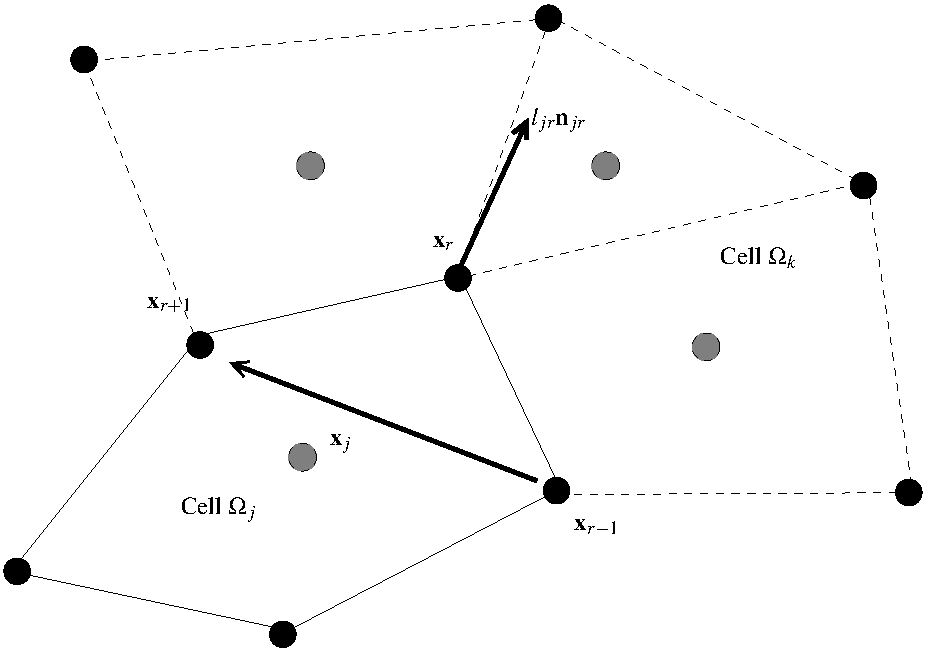
\includegraphics{atoc.pdf}}
\end{center}

\caption{Notation for node formulation. The corner length $l_{jr}$ 
and the corner normal $\njr$ are defined in equation (\ref{eq:not}).
The point $\x_j$ is an arbitrary point inside the cell, typically
the centroid of the cell or an averaged of the corners.
}
\end{figure}







The numerical approximation  
 of the problem  $\mathbf P^\eps$ that we study 
 is the JL-(b) scheme defined
in   \cite{glaceap}
\begin{equation}\label{eq:4}
\mathbf P_h^\eps:
\qquad \left\{ 
\begin{array}{l}
\displaystyle \mid\Omega_{j}\mid\frac{d}{dt} p_{j}^{\eps}+\frac{1}{\varepsilon}
\sum_{r}(l_{jr}\ur^{\eps},\njr)=0\\
\displaystyle \mid
\Omega_{j}\mid\frac{d}{dt}\uj^{\eps}+\frac{1}{\varepsilon}
\sum_{r} l_{jr} \njr    p_{jr}^{\eps}=-\frac{\sigma}{\varepsilon^{2}}\sum_{r}\widehat{
\beta}_{jr}\ur^{\eps},
\end{array}
\right.
\end{equation}
with initial data $p_j^{\eps}(0)=p_0(\mathbf{x}_j)$ and $\mathbf{u}_j^{\eps}(0) = -\eps\sigma^{-1}\nabla p_0(\mathbf{x}_j)$.
The fluxes are defined by the so-called 
corner problem 
\begin{equation}\label{eq:5}
\left\{ \begin{array}{l}
\displaystyle 
p_{jr}^{\eps}-p_j^\eps=
(\njr,    \uj^{\eps}-\ur^{\eps}
)-\frac{\sigma}{\varepsilon}( \xr -\xj, \ur^{\eps}), 
\\
\sum_{j}\ljr
p_{jr}^{\eps}\njr=0.
 \end{array}\right.
\end{equation}
This corner problem has been introduced in 
\cite{glaceap} as a multidimensional version
of the 1D Jin-Levermore technique   \cite{jinlev}.
Its solution is provided by the solution
of the  linear system
\begin{equation*} \label{eq:5bis}
\displaystyle \left( \sum_{j}\alj+ 
\sum_{j}\frac{\sigma}{\varepsilon}\bej\right)\ur^{
\eps}= \sum_{j}\ljr
p_j^{\eps}\njr+\sum_j\alj\uj^{\eps},
\end{equation*}
 where the geometry of the mesh is sued to define the  
  matrices  
$\alj$ and $\bej$ 
\begin{equation}\label{eq:6}
\alj=\ljr\njr\otimes\njr,\mbox{ and
}\bej=\ljr\njr\otimes(\xr-\xj) .
\end{equation}
We will use the notations
$A_j=\sum_r\alj$, $A_r=\sum_j\alj$ and
$B_r=\sum_j\bej$. 
By comparison with the scheme $P_h^\eps$ in dimension one, one sees at once
that the multi-dimensional scheme (\ref{eq:4}-\ref{eq:6})  is  more 
tricky than the 1D scheme (\ref{schema1}-\ref{eq:fflux}).



Starting from (\ref{eq:4}) and taking into account of the definitions of
the fluxes (\ref{eq:5}) and also the identity $\sum_r l_{jr} \njr=0$,
the scheme $\mathbf P_h^\eps$ can also be rewritten as
\begin{equation}\label{eq:4bis}
\mathbf P_h^\eps:
\qquad
\left\{ 
\begin{array}{l}
\displaystyle \mid\Omega_{j}\mid\frac{d}{dt} p_{j}^{\eps}+\frac{1}{\varepsilon}
\sum_{r}(l_{jr}\ur^{\eps},\njr)=0\\
\displaystyle \mid
\Omega_{j}\mid\frac{d}{dt}\uj^{\eps}+\frac{1}{\varepsilon}
\sum_{r}l_{jr} (\njr,\uu_r^{\eps} -\uu_j^{\eps})\njr=0
\end{array}
\right.
\end{equation}
When $\eps \rightarrow 0$
the scheme $\mathbf P_h^\eps$ admits the limit diffusion scheme 
$\mathbf P_h^0$ 
\begin{equation}\label{diffglace}
\mathbf P_h^0:
\qquad\left\{ \begin{array}{l}
\displaystyle \left| \Omega_j 
\right| \frac{d}{dt} p_j+ 
\sum_{r} l_{jr}\bigg( 
\vv_r,\njr\bigg)=0,\\
\displaystyle \vv_r=\frac{1}{\sigma} B_r^{-1}
\sum_{j}l_{jr}p_j\njr,
\end{array}\right.
\end{equation}
with $B_r=\sum_{j}l_{jr}\njr\otimes(\xr-\xj)$.
We  define additionally $\vv_j$ by a kind of mean
$$
\left( \sum_r \alj \right) \vv_j=\sum_r \alj
\vv_r.
$$
This is well defined since the matrix
$\sum_r \alj$ is  symetric positive by definition of the $\alj$.

\subsection{Definition of $\mathbf{DA}_h^\eps$}


We define now that is  call thereafter the "diffusion approximation" 
scheme.
We just neglect the time derivative
in the second equation, that we make
 $\partial_t\uj^{\eps}=0$ for (\ref{eq:4bis}). It
leads to the scheme
\begin{equation}\label{das}
\mathbf{DA}_h^\eps:
\quad
\left\{ 
\begin{array}{l}
\displaystyle \mid\Omega_{j}\mid\frac{d}{dt} p_{j}^{\eps}+\frac{1}{\varepsilon}
\sum_{r}(l_{jr}\ur^{\eps},\njr)=0\\
\frac{1}{\varepsilon} \sum_{r}l_{jr} (\njr,\uu_r^{\eps} -\uu_j^{\eps})\njr=0\\
\displaystyle \left( \sum_{j}\alj+ 
\sum_{j}\frac{\sigma}{\varepsilon}\bej\right)\ur^{
\eps}= \sum_{j}\ljr
p_j^{\eps}\njr+\sum_j\alj\uj^{\eps}
\end{array}
\right.
\end{equation}
This  scheme depends of
two parameters, the size of the mesh $h$ and the small parameter 
$\eps$.
We notice that
$\mathbf{DA}_h^\eps\neq \mathbf P_h^0$ for $\eps> 0$, and that 
$\lim_{\eps\rightarrow 0^+} \mathbf{DA}_h^\eps = \mathbf P_h^0$.
The initial data for \eqref{das} is $p_j^{\eps}(0)=p_0(\mathbf{x}_j)$. There is no 
need of initial data for $(u_j^{\eps}(0))$, which will be obtained 
 as a function of $(p_j^{\eps}(0))$ by solving a linear system.


\subsection{Mesh assumptions}


 \begin{figure}[h!]
 \begin{center}
 \scalebox{0.8}{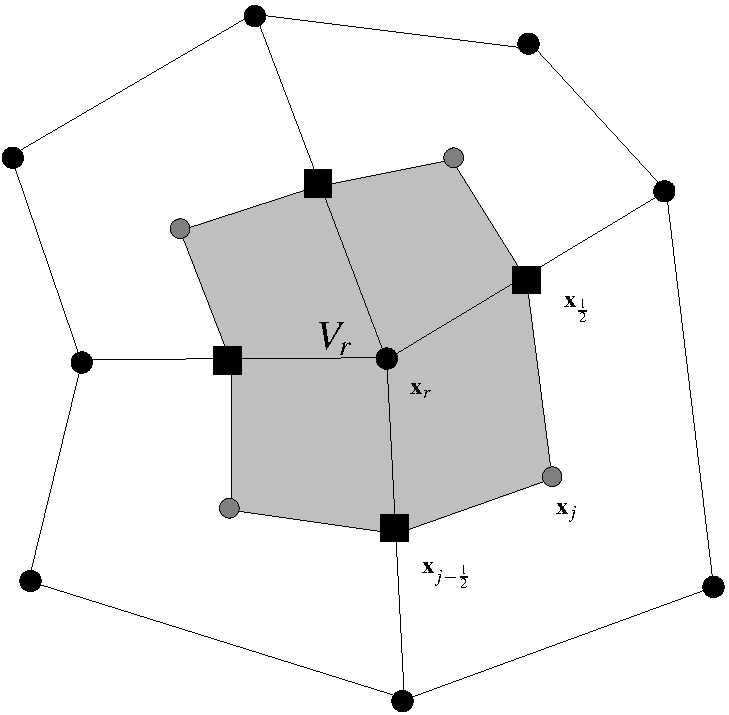
\includegraphics{vr.pdf}}
 \end{center}
 \caption{Definition of the control volume $V_r$ around
 vertex $\mathbf{x}_r$.
 The control volume  around the vertex $\mathbf{x}_r$
 is defined by the closed loop
 that joins the center of the cells ($\mathbf{x}_j$'s) and the middle
 of the edges ($\mathbf{x}_{j+\frac12}$'s).}
 \label{figcv}
 \end{figure}


The characteristic length of the mesh is 
\begin{equation*} \label{eq:d6}
h=\max_j \left( \mbox{diam}(\Omega_j)  \right).
\end{equation*}
By definition  there exists  a constant $C>0$ such that 
\begin{equation} \label{eq:d7}
l_{jr}\leq Ch , \qquad \forall j,r.
\end{equation}
The control volume $V_r$ 
around the vertex $\mathbf x_r$ is 
defined by the closed loop
$
\dots, \mathbf{x}_{j-\frac12}, \mathbf{x}_j,\mathbf{x}_{j+\frac12},\dots$.
Here  the $\mathbf{x}_j$'s are the center of the cells, and the 
$\mathbf{x}_{j+\frac12}$'s are the middle of the edges around the vertices
$\mathbf{x}_r$.
A typical example is depicted in  figure \ref{figcv}. 

Additional geometrical assumptions are always
necessary in dimension greater than one to guarantee
some minimal regularity of the mesh.
We make  the usual assumptions
 listed below from 1 to 3.
The two last items are more specific.

\begin{hyp}\label{geometrie}
Our geometrical assumptions  will be the following
\begin{enumerate}
\item The mesh is regular in the sense that
there are
two constants $C_1,C_2>0$ such that
\begin{equation} \label{eq:d5}
C_1 h^2 \leq \left| \Omega_j \right| \leq C_2 h^2, \quad \forall j\qquad
\mbox{ uniformly with respect to  }h.
\end{equation}
and that 
\begin{equation} \label{eq:d5.2}
C_1 h^2 \leq \vert V_r \vert \leq C_2 h^2, \quad \forall r\qquad
\mbox{ uniformly with respect to  }h.
\end{equation}
We recall that $V_r$ is the volume control (centered on $\x_r$) and $\Omega_j$
is the cell $j$.
\item The numbers of cells which share  a node $r$ is
bounded independently of $h$, which means there exists 
$P\in \mathbb N$ independent of $h$ such that
\begin{equation}\label{nbmr} 
\sum_j \delta_{jr}\leq P.
\end{equation}
For example, for a structured mesh of quadrangular cells $P=4$.
 
 \item For  each cell of the mesh, the  number of edges is
bounded independently of $h$, or equivalently the numbers of vertices for a cell
 is bounded independently of $h$.

\item 
A consequence of the items 1-3 
is that there exists 
 a constant
$\beta >0 $ such that 
\begin{equation}\label{geom4}
(A_j\uu, \uu)\geq \beta h (\uu,\uu).
\end{equation}
It can be proved with a geometrical  identity that we borrow
 from \cite{de10}  (proposition 8).

\item  The matrix $B_r$ is positive and that there exists a
constant $\alpha >0 $ independent of r such that 
\begin{equation}\label{geom3}
(B_r \uu, \uu)=(B^s_r \uu, \uu)\geq \alpha \vert
V_r\vert (\uu,\uu)
\end{equation}
where $B^s_r=\frac12 (B_r+B_r^t)$ is the symmetric part of $B_r$.
Square meshes satisfy (\ref{geom3}).
This assumption is however not trivial to check in the general case.
We point out  \cite{glaceap} where
 sufficient conditions such that (\ref{geom3}) is satisfied
can be found; in particular it is shown 
that  triangular meshes with all angles greater than $12$ degrees
satisfy it. 
\end{enumerate}
\end{hyp}


We  use the convention that the quadratic norm
of any cell centered quantity $f=(f_j)_{j\in {\rm Cells}}$ is
$\|f\|_{L^2(\Omega)}=\sqrt{\sum_j |\Omega_j| |f_j|^2   }$, while the quadratic
norm of any vertex based quantity $g=(g_r)_{r\in {\rm Vertices}}$ is
$\|g\|_{L^2(\Omega)}=\sqrt{\sum_r |V_r| |g_r|^2   }$.
Useful  quantities  are
\begin{itemize}
\item $\mathbf V_h^\eps=\left(p^\eps_j, \uu^\eps_j \right)_
{j\in {\rm Cells}}$ is the solution of $\mathbf P_h^\eps$.
\item 
$\mathbf V^\eps=\left(p^\eps(\x_j), \uu^\eps(\x_j)  \right)_
{j\in {\rm Cells}}$ is the solution of $\mathbf P^\eps$,
\item $\mathbf W_h^\eps=\left(p^\eps_j, \uu^\eps_j \right)_
{j\in {\rm Cells}}$ is the solution of $\mathbf{DA}_h^\eps$.
Notice that an abuse of notations is been made with the solution
of $\mathbf P_h^\eps$.
\item $\mathbf W^\eps= \left(p(\x_j),-\frac\eps\sigma \nabla p(\x_j)  \right)_
{j\in {\rm Cells}} $ is the solution of $\mathbf P^0$.
\end{itemize}
With these notations,  (\ref{ine3}) is rewritten as
\begin{equation} \label{eq:enc22}
\|\W^\eps-\mathbf V^\eps\|
_{ L^2([0,T]\times L^2(\Omega)   ) } \leq C \eps.
\end{equation}


\subsection{Study of $\| \mathbf 
P_h^\varepsilon -\mathbf P^\varepsilon \|_{\rm naive}$}


In this part, we exploit the hyperbolic nature
of both 
$\mathbf P^\varepsilon$ and $\mathbf P_h^\varepsilon $.
We first prove the $L^{2}$ stability of  the scheme JL-(b) defined 
in (\ref{eq:4},\ref{eq:5}).


\begin{pro}[Stability] \label{propesti} Under the geometrical assumption (\ref{geom3}), the
semi-discrete general JL-(b) scheme defined by (\ref{eq:4},\ref{eq:5})  is
stable in the $L^2$ norm in the sense that $\frac{d}{dt}
 \vert\vert \V^{\eps}_{h}(t)
\vert\vert \leq 0$.
 Moreover we have the bounds
\begin{equation}\label{gggg}
\frac{\sigma}{\eps^2}\vert\vert \uu_r^{\eps} \vert\vert_{L^2([0,T]\times \Omega)}\leq
C 
\vert\vert
V^{\eps}_h(0)\vert\vert_{L^2( \Omega)}, \qquad C>0,
\end{equation}
\begin{equation}\label{gs}
\int_0^T\sum_j \sum_r
l_{jr}(\njr,(\uj^\eps-\ur^\eps))^{2} dt\leq C  \eps \vert\vert
\mathbf V^{\eps}_h(0)\vert\vert^2_{L^2( \Omega)}. 
\qquad C>0.
\end{equation}
\end{pro}

\begin{proof}
We define the functions $p^{\eps}_h$ and $\uu^{\eps}_h$  by
$p^{\eps}_h=p_j$ and $\uu^{\eps}_h=\uj$  on $\Omega_j$.
We set for convenience $E(t)= \vert\vert \V^{\eps}_{h}(t)
\vert\vert^2$.
 One has
$$
E^{'}(t)=\displaystyle \frac12  \int_{\Omega} \frac{d}{dt}( \mid
p^{\eps}_{h} \mid^{2}+
(\uu^{\eps}_{h},\uu^{\eps}_{h}))=\int_{\Omega}
p^{\eps}_{h}\frac{d}{dt}p^{\eps}_{h}+(\uu^{\eps}_{h},\frac{d}{dt
}\uu^{\eps}_{h})
=\displaystyle \sum_{j} \left| \Omega_j \right|
p_{j}^{\eps}\frac{d}{dt} p_{j}^{\eps}+(\uj^{\eps},\frac{d}{dt}\uj^{\eps}).
$$
Using the definition of scheme 
\begin{equation}\label{eq:ds1}
\displaystyle E^{'}(t)=-\frac{1}{\varepsilon}
\sum_{j}\sum_{r}l_{jr}p_{j}^{\eps}(\ur^{\eps},\njr)
-\frac{1}{\varepsilon
}\sum_{j}\sum_{r}(l_{jr}p_{j,r}^{\eps} \njr,\uj^{\eps})
-\frac{\sigma}{\varepsilon^{2}}
\sum_{j}\sum_r (\widehat{\beta}_{jr}\ur^{\eps},\uj^{\eps}).
\end{equation}
Using (\ref{eq:5}) we expand the second term of the previous equation 
\begin{equation}\label{eq:ds2}
\displaystyle
\sum_{j}\sum_{r}(
l_{jr}p_{j,r}^{\eps}\njr
,\uj^{\eps})=\sum_{j}\sum_{r}l_{jr}p_{j}^{\eps}
(\uj^{\eps},\njr)+\sum_{j}\sum_{r}(\widehat {\alpha}_{jr}(\uj^{\eps}
-\ur^{\eps}),\uj^{\eps})-\frac{\sigma}{\varepsilon}\sum_{j}\sum_{r}({
\widehat\beta}_{jr}\ur^{\eps},\uj^{\eps}).
\end{equation}
Since $\sum_{r}l_{jr}\njr=0$ the first term of (\ref{eq:ds2}) is
zero.
Summing on r the second equation of (\ref{eq:5}) and permuting the sums, we show
that $0=
 \displaystyle \sum_{j}\sum_{r}l_{jr}p_{jr}(\ur,\njr)$ which yields that
\begin{equation}\label{eq:ds3}
0=
 \displaystyle \sum_{j}\sum_{r}l_{jr}p_{j}^{\eps}(\ur^{\eps},\njr)-
\sum_{j}\sum_{r}((\widehat
{\alpha}_{jr}+\frac{\sigma}{\varepsilon}\widehat
{\beta}_{jr})\ur^{\eps},\ur^{\eps})
+\sum_{j}\sum_{r}(\widehat{\alpha}_{jr}\uj^{\eps},\uu_{r
}^{\eps}).
\end{equation}
Plugging (\ref{eq:ds2}) and (\ref{eq:ds3}) in (\ref{eq:ds1}) and permuting the
sums in $E'(t)$ gives
\begin{equation*}\label{rresti}
E^{'}(t)=\displaystyle -\frac{1}{\varepsilon}
\sum_{j}\sum_{r}( \widehat{\alpha}_{jr}(\uj^{\eps}-\ur^{\eps}),\uj^{\eps}
-\ur^{\eps})- \frac{\sigma}{\varepsilon^{2}}
\sum_{r}\sum_{j}(\widehat {\beta}_{jr}\ur^{\eps},\ur^{\eps})
\end{equation*}
which gives
\begin{equation}\label{eq:ds4}
\displaystyle
E^{'}(t)+\frac{1}{\varepsilon}\sum_{r}\sum_{j}l_{jr}(\njr,(\uu^{\eps}
_{j}-\ur^{\eps}))^{2}+ \frac{\sigma}{\varepsilon^{2}}
\sum_{r}(B_r\ur^{\eps},\ur^{\eps})= 0.
\end{equation}
By geometrical assumption  (\ref{geom3}) we have $E^{'}(t)\leq 0$, that is the
$L^2$ stability, and
by integrating this equality on $[0,T]$ we obtain
\begin{equation*}\label{eq:ds5}
\displaystyle
E(T)+\int_0^T\frac{1}{\varepsilon}\sum_{r}\sum_{j}l_{jr}(\njr,
(\uj^{\eps}-\ur^{\eps}))^{2}+ \int_0^T\frac{\sigma}{\varepsilon^{2}}
\sum_{r}(B_r\ur^{\eps},\ur^{\eps})=E(0)
\end{equation*}
Using again the geometrical assumption  (\ref{geom3}) for the terms
$(B_r\ur^{\eps},\ur^{\eps})$ we have
\begin{equation*}\label{eq:ds6}
\displaystyle
E(T)+\int_{0}^T\frac{1}{\varepsilon}\sum_{r}\sum_{j}l_{jr}(\njr,
(\uj^{\eps}-\ur^{\eps}))^{2}+ \alpha
\int_{0}^T\frac{\sigma}{\varepsilon^{2}} \sum_{r}\vert V_r\vert
\ \vert\ur^{\eps}\vert^2\leq E(0)
\end{equation*}
which gives (\ref{gggg}) and (\ref{gs}).
\begin{comment}
The last inequality can be obtained as follows.
One has
$$
\begin{array}{ll}
\vert\vert \uu_j^{\eps} \vert\vert_{L^2( \Omega)}&
\leq 
C \sum_j h^2 \vert\mathbf u_j ^\eps \vert^2
\\
& \leq 
C h  \sum_j \sum_r l_{jr} 
( \mathbf n_{jr}, \mathbf{u}_j^\eps    )^2
\\
& \leq 
C h  \sum_j \sum_r l_{jr} 
2 ( \mathbf n_{jr}, \mathbf u_r ^\eps    )^2
+
C h  \sum_j \sum_r l_{jr} 
2 ( \mathbf n_{jr}, \mathbf u_j ^\eps  - \mathbf u_r ^\eps    )^2 \\
&
\leq C
\vert\vert \uu_r^{\eps} \vert\vert_{L^2(\Omega)} 
+
C h  \sum_j \sum_r l_{jr} 
2 ( \mathbf n_{jr}, \mathbf u_j ^\eps  - \mathbf u_r ^\eps    )^2 .
\end{array}
$$
Using inequalities  (\ref{gggg}) and (\ref{gs}), one gets
$$
\vert\vert \uu_j^{\eps} \vert\vert_{L^2( [0,T]\times \Omega)}^2
\leq C 
\vert\vert \uu_r^{\eps} \vert\vert_{L^2( [0,T]\times \Omega)}^2
+C\int_0^T 
h  \sum_j \sum_r l_{jr} 
 ( \mathbf n_{jr}, \mathbf u_j ^\eps  - \mathbf u_r ^\eps    )^2 
\leq 
C ( \eps^2  + h \eps) \vert\vert
\mathbf V^{\eps}_h(0)\vert\vert^2_{L^2( \Omega)}.
$$
\end{comment}
The proof is ended.
\end{proof}

Our goal now is to prove the following result 
which will be the consequence
of propositions \ref{pro:conv1} to \ref{pro:conv2}.
This part is the more technical one of the paper, but is essential
to be able to use the general strategy of proposition
\ref{prop:1} with convenient exponents. 
As one will see below, the convergence estimate
(\ref{eq:veps2}) is not trivial. It indicates that, 
for a problem with $O(\varepsilon^{-2})$ terms, a scheme 
converges, with $h$, with  at rate $O(\varepsilon^{-\frac12})$ with respect to
$\eps$.

\begin{proposition}[Convergence]\label{ein_prosit}
There exists a constant $C(T, \sigma)>0$ 
      such that the following estimate holds
\begin{equation} \label{eq:veps2}
\|\V^{\eps}_h-\V^{\eps}\|_{L^\infty( [0,T]\times L^2  (\Omega) )}\leq
C(T, \sigma)\|  \mathbf V ^\eps (0) \|_  { H^3(\Omega)  }
\sqrt{\frac h \eps}.
\end{equation}
\end{proposition}
In the whole proof, we will use a constant $C>0$ large enough.
 Like in 1D, we use the method introduced by Mazeran \cite{Mazeran}. 
We introduce
$\mathscr{E}(t)=\frac12 \|\V^{\eps}-\V^{\eps}_h\|_{L^2(\Omega)}^2$.
As for the 1D proof and for the sake of simplicity, for any quantity $q$,   $q'$ stands indifferently for  $\frac{d}{dt}q $ or $\partial_t q $.

\begin{pro} \label{pro:conv1}
One has the formula
\begin{equation} \label{eq:ee1}
\begin{aligned}
\mathscr{E}'(t) &=
-\frac{1}{\eps}\sum_{j,r}l_{j,r}(\mathbf{n}_{j,r},\mathbf{u}_j^{\eps}-\mathbf{u}
_r^{\eps})^2 \\
&+ \frac{1}{\eps} \sum_j \sum_r \bigg(
l_{j,r}(\mathbf{u}_r^{\eps}-\mathbf{u}_j^{\eps}),\mathbf{n}_{j,r} \bigg)
\delta_{j,r}(p^{\eps}) +\frac{1}{\eps} \sum_j \sum_r \bigg( 
 l_{j,r}\mathbf{n}_{j,r} ( p_{jr}^{\eps}  - p_j^{\eps}) \: , \:
\delta_{j,r}(\uu^{\eps}) \bigg) \\
&+\frac{1}{\eps}\sum_j \sum_r  |\Gamma_{j,r} | p_j^{\eps} (\mathbf{n}_{j,r} ,
\tilde{\delta}_{j,r}(\uu^{\eps}) ) + \frac{1}{\eps}\sum_j \sum_r |\Gamma_{j,r} | \bigg(
\mathbf{u}_j^{\eps} , \mathbf{n}_{j,r} \tilde{\delta}_{j,r}(p^{\eps}) \bigg) \\
&+\frac{\sigma}{\eps^2} \sum_r \sum_j 
\bigg(\widehat{\beta}_{j,r}\mathbf{u}_r^{\eps}  \: , \:
\frac{1}{|\Omega_j|}\int_{\Omega_j} \uu^{\eps} d\x \bigg)
+\frac{\sigma}{\eps^2}\sum_j\bigg(  \mathbf{u}_j^{\eps} ,
\int_{\Omega_j}\uu^{\eps}d\x \bigg) \\
&-\frac{\sigma}{\eps^2}\sum_j\int_{\Omega_j}(\uu^{\eps},\uu^{\eps}
)d\x -\frac{\sigma}{\eps^2}\sum_{r}
(B_{r}\mathbf{u}_r^{\eps},\textbf{u}_r^{\eps})
\end{aligned}
\end{equation}
where  the extra notations are:
$\delta_{j,r}(f)= \frac{1}{|\Omega_j|}\int_{\Omega_j} f d\x
-f(\x_{r})$ is an interpolation error term that compares mean values and point 
values;
$\Gamma_{j,r}=[\x_{r},\x_{r+1}]$ is the edge
oriented toward the outside of the cell $j$, with
length $|\Gamma_{j,r} | $; and $\tilde{\delta}_{j,r}(h)=
\frac1{|\Gamma_{j,r}| } \int_{\Gamma_{j,r}} h d s
-\frac{h(\textbf{x}_{r})+h(\textbf{x}_{r+1})}{2}$ is another
interpolation error contribution that compares the  mean value and the mid sum,
on the edge.
\end{pro}



\begin{proof}
We first consider  the time  derivative
\begin{equation*} \label{eq:eetoile}
\begin{array}{l}
\mathscr{E}'(t)
=\underbrace{\int_{\Omega}(p_h^{\eps}(p_h^{\eps})'+(\uu_h^{\eps},(\textbf{u}
_h^{\eps})'))d\x}_{D_1}+ \underbrace{
\int_{\Omega}(p^{\eps}(p^{\eps})'+(\textbf{u}^{\eps},(\textbf{u}^{\eps})'))d\x}_{
D_2} \\
\hspace{0.8cm}+ \underbrace{\int_{\Omega}
(-(p_h^{\eps})'p^{\eps}-((\textbf{u}_h^{\eps})',\textbf{u}^{\eps}))d\x}_{D_3} 
+ \underbrace{\int_{\Omega}
(-p_h^{\eps}(p^{\eps})'-(\textbf{u}_h^{\eps},(\textbf{u}^{\eps})'))d\x}_{D_4}.
\end{array}
\end{equation*}
One has thanks to  (\ref{eq:ds4})
$$
D_1
=-\frac{1}{\eps}\sum_{j,r}l_{j,r}(\textbf{n}_{j,r},\textbf{u}_j^{\eps}-\textbf{u}
_r^{\eps})^2-\frac{\sigma}{\eps^2}\sum_{r}
( B_r\textbf{u}_r^{\eps},\textbf{u}_r^{\eps}).
$$
One also directly has
\begin{equation*}
D_2 =
-\frac{\sigma}{\eps^2}\int_{\Omega}(\uu^{\eps},\uu^{\eps})d\x =
-\frac{\sigma}{\eps^2}\sum_j\int_{\Omega_j}(\uu^{\eps},\uu^{\eps}
)d\x.
\end{equation*}
Then,  using the  definition (\ref{eq:4},\ref{eq:5}) of the scheme we have
\begin{equation*}
\begin{array}{l}
D_3 = \frac{1}{\eps} \sum_j \sum_r \bigg(
l_{j,r}\textbf{u}_r^{\eps},\textbf{n}_{j,r} \bigg) 
\frac{1}{|\Omega_j|}\int_{\Omega_j} p^{\eps} dx \\
\hspace{1cm}+\frac{1}{\eps} \sum_j \bigg( \sum_r
l_{jr} \mathbf n_{jr} p_{j,r}^{\eps}+\frac{\sigma}{\eps} \sum_r
\widehat{\beta}_{j,r}\textbf{u}_r^{\eps}  \: , \:
\frac{1}{|\Omega_j|}\int_{\Omega_j} \uu^{\eps} d\x \bigg) 
\end{array}
\end{equation*}
Since $\sum_r l_{jr} \mathbf n_{jr}=0$,  we can write
\begin{equation*}
\begin{array}{ll}
D_3= &  \frac{1}{\eps} \sum_j \sum_r \bigg(
l_{j,r}(\textbf{u}_r^{\eps}-\textbf{u}_j^{\eps}),\textbf{n}_{j,r} \bigg) 
\frac{1}{|\Omega_j|}\int_{\Omega_j} p^{\eps} dx \\
& + \frac{1}{\eps} \sum_j \bigg( \sum_r 
l_{jr} \mathbf n_{jr} (p_{j,r}^{\eps}
-
p_j^{\eps})  \: , \: \frac{1}{|\Omega_j|}\int_{\Omega_j}
\uu^{\eps} d\x \bigg) \\
& +\frac{\sigma}{\eps^2} \bigg( \sum_r \sum_j\widehat{\beta}_{j,r}\textbf{u}_r^{\eps} 
\: , \: \frac{1}{|\Omega_j|}\int_{\Omega_j} \uu^{\eps} d\x \bigg) .
\end{array}
\end{equation*}
One gets
\begin{equation*}
\begin{array}{l}
D_3 =\frac{1}{\eps} \sum_j \sum_r \bigg(
l_{j,r}(\textbf{u}_r^{\eps}-\textbf{u}_j^{\eps}),\textbf{n}_{j,r} \bigg)
\delta_{j,r}(p^{\eps})+\frac{1}{\eps} \sum_j \sum_r \bigg( 

l_{jr} \mathbf n_{jr} (p_{j,r}^{\eps}
-
p_j^{\eps}) \: ,
\:\delta_{j,r}(\uu^{\eps}) \bigg) \\
\hspace{0.6cm}+ \frac{1}{\eps} \sum_j \sum_r \bigg(
l_{j,r}(\textbf{u}_r^{\eps}-\textbf{u}_j^{\eps}),\textbf{n}_{j,r} \bigg)
p^{\eps}(\x_r)+ \frac{1}{\eps} \sum_j \sum_r \bigg(  
l_{jr} \mathbf n_{jr} (p_{j,r}^{\eps}
-
p_j^{\eps})  \: , \:  \uu^{\eps}(\textbf{x}_{r}) \bigg) \\
\hspace{0.6cm}+\frac{\sigma}{\eps^2} \bigg( \sum_r \sum_j
\widehat{\beta}_{j,r}\textbf{u}_r^{\eps}  \: , \:
\frac{1}{|\Omega_j|}\int_{\Omega_j} \uu^{\eps} d\x \bigg) .
\end{array}
\end{equation*}
We have the identities $\sum_{j,r}\ljr \njr 
=0$
and  $\sum_j  l_{jr} \mathbf n_{jr} p_{j,r}^{\eps}=0$ by definition
(\ref{eq:5}).
Therefore one can simplify the third and fourth term
in the previous expression and get 
\begin{equation*}
\begin{aligned}
D_3  & =  \frac{1}{\eps} \sum_j \sum_r \bigg(
l_{j,r}(\textbf{u}_r^{\eps}-\textbf{u}_j^{\eps}),\textbf{n}_{j,r} \bigg)
\delta_{j,r}(p^{\eps})+\frac{1}{\eps} \sum_j \sum_r \bigg( 
l_{jr} \mathbf n_{jr} (p_{j,r}^{\eps}
-
p_j^{\eps}) \: , \:
\delta_{j,r}(\uu^{\eps}) \bigg) \\
& - \frac{1}{\eps} \sum_j \sum_r \bigg(
l_{j,r}\textbf{u}_j^{\eps},\textbf{n}_{j,r} \bigg) p^{\eps}(\x_r)- \frac{1}{\eps}
\sum_j \sum_r \bigg( l_{j,r}p_j^{\eps}\textbf{n}_{j,r} \: ,\:
\uu^{\eps}(\textbf{x}_{r}) \bigg)\\
 & + \frac{\sigma}{\eps^2} \bigg( \sum_r
\sum_j\widehat{\beta}_{j,r}\textbf{u}_r^{\eps}  \: , \:
\frac{1}{|\Omega_j|}\int_{\Omega_j} \uu^{\eps} d\x \bigg) .
\end{aligned}
\end{equation*}
We now look at $D_4$. By definition, one has
\begin{equation*}
D_4= \frac{1}{\eps}\sum_j p_j^{\eps} \sum_r \int_{\Gamma_{j,r}}
(\uu^{\eps},\tnjr)d\sigma + \frac{1}{\eps}\sum_j
\bigg( \textbf{u}_j^{\eps} , \bigg( \sum_r \int_{\Gamma_{j,r}} p^{\eps}
\tnjr d\sigma
+\frac{\sigma}{\eps}\int_{\Omega_j}\uu^{\eps} d\x\bigg) \bigg)
\end{equation*}
where $\tnjr$ is the normal to the edge
$\Gamma_{j,r}=[\x_{r},\x_{r+1}]$ oriented toward the outside of the cell $j$. 
This expression needs an important manipulation which
is to approximate the integral on edges by corner values.
This necessary manipulation is one of the ideas that was introduced
in \cite{Mazeran} in order to proceed to the numerical
analysis of such corner based finite volume schemes.
This is why  interpolation terms  $\tilde{\delta}_{j,r}(h)= 
\frac1{|\Gamma_{jr}|}\int_{\Gamma_{j,r}} h
- \frac{h(\textbf{x}_{r})+h(\textbf{x}_{r+1})}{2}$ are introduced.
One gets after an algebraic manipulation 
\begin{equation*}
\begin{aligned}
D_4 &= \frac{1}{\eps}\sum_j \sum_r |\Gamma_{j,r}|   p_j^{\eps} \bigg( \tnjr
,\tilde{\delta}_{j,r}(\uu^{\eps}) \bigg) +\frac{1}{\eps}\sum_j \sum_r
|\Gamma_{j,r}| 
\bigg( \textbf{u}_j^{\eps} ,
\tnjr\tilde{\delta}_{j,r}(p^{\eps})\bigg) +
\frac{\sigma}{\eps^2}\sum_j\bigg(  \textbf{u}_j^{\eps} ,
\int_{\Omega_j}\uu^{\eps} \bigg)\\
&+ \frac{1}{\eps}\sum_j \sum_r  |\Gamma_{j,r}| p_j^{\eps} \bigg(
\tnjr ,\frac{\uu^{\eps}(\textbf{x}_{r})+\uu^{\eps}(\textbf{x}_{r+1})}{2}
\bigg) + \frac{1}{\eps}\sum_j \sum_r |\Gamma_{j,r}| \bigg( \textbf{u}_j^{\eps} ,
\tnjr
\frac{p^{\eps}(\textbf{x}_{r})+p^{\eps}(\textbf{x}_{r+1})}{2}\bigg) 
\end{aligned}
\end{equation*}
By definition (\ref{eq:not}),
$\njr\ljr=\frac{\tilde{n}_{j,r}|\Gamma_{j,r}|+\tilde{n}_{j,r-1}|\Gamma_{j,r-1}|}
{2}$, so one can see that 
$$
\sum_j \sum_r |\Gamma_{j,r}|  p_j^{\eps} \bigg(
\tnjr ,\frac{\uu^{\eps}(\textbf{x}_{r})+\uu^{\eps}(\textbf{x}_{r+1})}{2}
\bigg)= \sum_j \sum_r  l_{jr} p_j^{\eps} \big( \njr ,\uu^{\eps}(\textbf{x}_{r}) \big).
$$ 
It yields a slightly simpler expression
$$
\begin{aligned}
D_4 &= \frac{1}{\eps}\sum_j \sum_r |\Gamma_{j,r}|   p_j^{\eps} \bigg( \tnjr
,\tilde{\delta}_{j,r}(\uu^{\eps}) \bigg) +\frac{1}{\eps}\sum_j \sum_r
|\Gamma_{j,r}| 
\bigg( \textbf{u}_j^{\eps} ,
\tnjr\tilde{\delta}_{j,r}(p^{\eps})\bigg) +
\frac{\sigma}{\eps^2}\sum_j\bigg(  \textbf{u}_j^{\eps} ,
\int_{\Omega_j}\uu^{\eps} \bigg)\\
&+ \frac{1}{\eps}
\sum_j \sum_r  l_{jr} p_j^{\eps} \big( \njr ,\uu^{\eps}(\textbf{x}_{r}) \big)
 + \frac{1}{\eps}\sum_j \sum_r \ljr p^{\eps}(\textbf{x}_{r})\big(\njr ,\textbf{u}_j^{\eps}\big) 
\end{aligned}
$$
One can now compute the sum  $D_3+D_4$
\begin{equation*}
\begin{aligned}
D_3+D_4 &= \frac{1}{\eps} \sum_j \sum_r \bigg(
l_{j,r}(\textbf{u}_r^{\eps}-\textbf{u}_j^{\eps}),\textbf{n}_{j,r} \bigg)
\delta_{j,r}(p^{\eps}) +\frac{1}{\eps} \sum_j \sum_r \bigg( 
 l_{j,r}\textbf{n}_{j,r}  (p_{j,r}^{\eps}- p_j^{\eps})  \: , \:
\delta_{j,r}(\uu^{\eps}) \bigg) \\
&+\frac{1}{\eps}\sum_j \sum_r  |\Gamma_{jr}|
p_j^{\eps}
\bigg(\textbf{n}_{j,r},\tilde{\delta}_{j,r}(\uu^{\eps}) \bigg) +
\frac{1}{\eps}\sum_j \sum_r  |\Gamma_{jr}| \bigg( \textbf{u}_j^{\eps} , \textbf{n}_{j,r}
\tilde{\delta}_{j,r}(p^{\eps})\bigg)\\
&+\frac{\sigma}{\eps^2} \bigg( \sum_r \sum_j \widehat{\beta}_{j,r}\textbf{u}_r^{\eps}
 \: , \: \frac{1}{|\Omega_j|}\int_{\Omega_j} \uu^{\eps} d\x \bigg)
+\frac{\sigma}{\eps^2}\sum_j \bigg(  \textbf{u}_j^{\eps} ,
\int_{\Omega_j}\uu^{\eps} d\x\bigg).
\end{aligned}
\end{equation*}
One finally gets after rearrangement
the final result (\ref{eq:ee1}) for $\mathscr{E}'(t)
=D_1+D_2+D_3 +D_4$.
\end{proof}


Before going further in the examination of each term in the right hand side of
(\ref{eq:ee1}), it is worthwhile to notice that terms like $\delta_{jr}(\dots)$ and 
$\widetilde \delta_{jr}(\dots)$ 
are small in some  sense. For this  we recall the results taken from \cite{Mazeran}, chapter 4:

\begin{pro} \label{pro:interp}
For any funtion $q$ in $ H^3(\Omega)$,   using  Sobolev embeddings,
one has the inequalities
\begin{equation}\label{}
 \vert \delta_{jr}(q) \vert
 \leq 
  C  \| q \| _{ H^1(\Omega_j) }
\end{equation}
and
\begin{equation}
\vert \widetilde \delta_{jr}(q)\vert
\leq  
  C h^{3/2}  \| q \| _{ H^3(\Omega_j) }
\end{equation}
\end{pro}



Our aim is to now examine each term in the right hand side of
(\ref{eq:ee1}). Its  first line is already non positive.
We  look at the second line of (\ref{eq:ee1})  which we call
$E_1$. 
%%%%%%%%%%%%%%%%%%%%%%%%%%%%%%%%%%%%%%%%%%%%%%%%%%%%%%%%%%%%%%%%%%%%%%%%%%
\begin{pro}
One has
the bound with a constant $C$proportional to $  \|  \mathbf V ^\eps (0) \|^2_  { H^1(\Omega)  }$  
\begin{equation} \label{eq:bound1}
\int_0^T E_1(t)dt \leq 
\frac{\gamma}{\eps}\int_0^T\sum_{j,r}l_{j,r}(\textbf{n}_{j,r},\textbf{u}_j^{\eps}-\textbf{u}
_r^{\eps})^2 
+Ch(  \frac T {\gamma } +1).
\end{equation}
\end{pro}
\begin{proof}
We use a Young's inequality 
$ab\leq \frac\gamma2 a^2+\frac1{2\gamma} b^2$,with some positive constant$\gamma$ which will be defined later,   for the second term
and the definition of the fluxes (\ref{eq:5}) for the third term: we get
\begin{equation*}
\begin{aligned}
E_1 &\leq  \frac{\gamma }{2 \eps}\sum_{j,r}l_{j,r}(\textbf{n}_{j,r},\textbf{u}_j^{\eps}
-\textbf{u}_r^{\eps})^2 + \frac{1}{2\gamma\eps} \sum_j \sum_r l_{j,r}
\delta_{j,r}(p^{\eps})^2 \\
&+\frac{1}{\eps} \sum_j \sum_r \bigg(
\widehat{\alpha}_{j,r}(\textbf{u}_j^{\eps}-\textbf{u}_r^{\eps}) \: , \:
\delta_{j,r}(\uu^{\eps}) \bigg) -\frac{1}{\eps} \sum_j \sum_r \bigg(
\frac{\sigma}{\eps} \widehat{\beta}_{j,r}\textbf{u}_r^{\eps}\: , \:
\delta_{j,r}(\uu^{\eps} )\bigg) \\
\end{aligned}
\end{equation*}
 By definition of $\widehat{\alpha}_{j,r}$,
one rewrites
 $$
\sum_j \sum_r \bigg(
\widehat{\alpha}_{j,r}(\textbf{u}_j^{\eps}-\textbf{u}_r^{\eps}) \: , \:
\delta_{j,r}(\uu^{\eps}) \bigg) = \sum_j \sum_r 
\ljr(\njr , \textbf{u}_j^{\eps}-\textbf{u}_r^{\eps} )(\njr ,
  \delta_{j,r}(\uu^{\eps})).
$$ 
Another use of Young's inequality with the same coefficient $\gamma$ for this term
yields


\begin{equation*}
\begin{aligned}
E_1 &\leq  \frac{\gamma }{ \eps}\sum_{j,r}l_{j,r}(\textbf{n}_{j,r},\textbf{u}_j^{\eps}
-\textbf{u}_r^{\eps})^2 + \frac{1}{2\gamma\eps} \sum_j \sum_r l_{j,r}
\delta_{j,r}(p^{\eps})^2 \\
&+\frac{1}{2\gamma\eps} \sum_j \sum_r 
\
\delta_{j,r}(\uu^{\eps})^2 -\frac{1}{\eps} \sum_j \sum_r \bigg(
\frac{\sigma}{\eps} \widehat{\beta}_{j,r}\textbf{u}_r^{\eps}\: , \:
\delta_{j,r}(\uu^{\eps} )\bigg) \\
\end{aligned}
\end{equation*}




We now look at the last term of (\ref{eq:bound1}), which we call $W$.
One has, by definition of $\widehat{\beta}_{j,r}$
\begin{equation*}
W=-\frac{1}{\eps} \sum_j \sum_r \bigg( \frac{\sigma}{\eps}
\widehat{\beta}_{j,r}\textbf{u}_r^{\eps}\: , \: \delta_{j,r}(\uu^{\eps} )\bigg)
= -\frac{\sigma}{\eps^2} \sum_j \sum_r
\bigg((\ljr)^{\frac12 }\njr\otimes(\xr -\xj)
\textbf{u}_r^{\eps}\: , \: (\ljr)^{\frac12 }\delta_{j,r}(\uu^{\eps})
\bigg)
\end{equation*}
 Using the Cauchy-Schwarz inequality, we get
\begin{equation*}
\vert W \vert \leq \frac{\sigma}{\eps^2} \bigg(\sum_j \sum_r
\ljr  \bigg| 
\njr\otimes(\xr -\xj)
\textbf{u}_r^{\eps}
 \bigg|^2 \bigg)^{\frac12 } \bigg(\sum_j \sum_r
 \ljr  | \delta_{j,r}(\uu^{\eps})| ^2 \bigg)^{\frac12 } \\
\end{equation*}
Using the assumptions of the mesh, there exist a 
constant $C>0$ such that $|\xr -\xj|\leq Ch$.
 Using successively assumptions \eqref{eq:d5.2},\eqref{nbmr} and 
\eqref{geom3}, we get
\begin{equation*}\label{esti_beta}
\vert W \vert
\leq C \frac{\sigma h}{\eps^2}
\bigg( \sum_r \big( B_{r}\textbf{u}_r^{\eps},\textbf{u}_r^{\eps}\big)\bigg)^{\frac12} \bigg(\sum_j \sum_r    | \delta_{j,r}(\uu^{\eps})|^2 \bigg)^{\frac12 }.
\end{equation*}
and therefore
\begin{equation}\label{eq:bound2}
\vert W \vert
\leq C \frac{\sigma h}{2\eps^2}
\bigg( \sum_r \big( B_{r}\textbf{u}_r^{\eps},\textbf{u}_r^{\eps}\big)  +\sum_j \sum_r    | \delta_{j,r}(\uu^{\eps})|^2 \bigg).
\end{equation}
so that
\begin{equation} \label{eq:bound1bis}
\begin{aligned}
E_1 &\leq \frac{\gamma }{\eps}
\sum_{j,r}l_{j,r}(\textbf{n}_{j,r},\textbf{u}_j^{\eps}-\textbf{u}
_r^{\eps})^2 + \frac{1}{2\gamma\eps} \sum_j \sum_r l_{j,r}
\delta_{j,r}(p^{\eps})^2 \\
&+\frac{1}{2 \gamma \eps} \sum_j \sum_r l_{j,r}\bigg( \textbf{n}_{j,r} \: , \:
\delta_{j,r}(\uu^{\eps}) \bigg)^2 + C \frac{\sigma h}{2\eps^2}
\bigg( \sum_r \big( B_{r}\textbf{u}_r^{\eps},\textbf{u}_r^{\eps}\big)  +\sum_j \sum_r    | \delta_{j,r}(\uu^{\eps})|^2 \bigg)\\
\end{aligned}
\end{equation}

Furthermore, using the  classical interpolation results of proposition \ref{pro:interp} , there exists another constant $C\geq0$ such that 
\[
\sum_j \sum_r ( \delta_{j,r}\uu^{\eps})^2 \leq C \vert \vert \uu^\eps \vert\vert^2_{H^1(\Omega)}
.
\]
and
\[
\sum_j \sum_r l_{j,r} ( \delta_{j,r}p^{\eps})^2 \leq C h \vert \vert p^\eps \vert\vert^2_{H^1(\Omega)}
.
\]

So we obtain, after redefinition of all the constants $C$ 

$$
\int_0^T E_1 dt\leq 
\int_0^T \frac{\gamma}{\eps}
\sum_{j,r}l_{j,r}(\textbf{n}_{j,r},\textbf{u}_j^{\eps}-\textbf{u}
_r^{\eps})^2 
+\frac {Ch }{2\gamma \eps}\bigg(\vert \vert \uu^\eps \vert\vert^2_{H^1(\Omega)} +\vert \vert p^\eps \vert\vert^2_{H^1(\Omega)}  \bigg)
+C \frac{h\sigma}{2\eps^2}
\bigg(\sum_r \big( B_{r}\mathbf{u}_r^{\eps},\mathbf{u}_r^{\eps}\big) +  \vert \vert \uu^\eps \vert\vert^2_{H^1(\Omega)}\bigg)dt.
$$



Using  energy estimate (\ref{bee1})  for the the second  term of the rhs of the above inequality,    (\ref{gggg}) for the third term   and   (\ref{bee2}) for the last term,
one gets finally after simplifications and up to another redefinition  of the constant $C$(which is proportional to the $H^1(\Omega)$ norm of the initial data $\V_0$ and  is independent of the parameter $\sigma$)
\begin{equation} \label{eq:si1}
\int_0^T E_1(t)dt \leq 
\frac{\gamma}{\eps}\int_0^T\sum_{j,r}l_{j,r}(\textbf{n}_{j,r},\textbf{u}_j^{\eps}-\textbf{u}
_r^{\eps})^2 
+Ch(  \frac 1 {\gamma } +1).
\end{equation}
\end{proof}

%%%%%%%%%%%%%%%%%%%%%%%%%%%%%%%%%%%%%%%%%%%%%%%%%%%%%%%%%%%%%%%%%%%%%%%%%%

Now we consider the third line 
of  $\mathscr{E}'(t)$, which we call $E_2$.

\begin{pro} \label{pro:e2}
One has the bound
\begin{equation} \label{eq:si2}
\int_0^T E_2(t) dt \leq  \frac{CTh}{\eps} .
\end{equation} 

where the constant $C$ depends   on $\|  \mathbf V ^\eps (0) \|^2_  { H^3(\Omega)  }$
\end{pro}
\begin{proof}
$E_2=A+B$ is made of two contributions.
Making use of the second set of inequalities
of proposition \ref{pro:interp}, one gets concerning the first one
$$
| A|= \left |
\frac{1}{\eps}\sum_j \sum_r  |\Gamma_{j,r} | p_j^{\eps} (\mathbf{n}_{j,r} ,
\tilde{\delta}_{j,r}(\uu^{\eps}) ) 
\right |
\leq 
\frac{C}{\eps}  \sum_j h^{5/2} | p_j  ^\eps |
 \|  \mathbf V ^\eps (t) \|_  { H^3(\Omega_j)  }.
$$
And using the inequality $ab\leq \frac{1}{2}(a^2+b^2)$ 

$$
| A|\leq 
\frac{C_1}{\eps}  \sum_j h^{3} | p_j  ^\eps |^2 + \frac{C_2}{\eps} \sum_j h^{2} 
 \|  \mathbf V ^\eps (t) \|^2_  { H^3(\Omega_j)  }
 \leq 
\frac{hC_3}{\eps} \|  \mathbf V_h ^\eps (t) \|^2_  { L^2(\Omega)  } + \frac{C_2h^2}{\eps}  
 \|  \mathbf V ^\eps (t) \|^2_  { H^3(\Omega)  }.
$$
The $L^2$ stability  (\ref{gggg})  of the scheme $\mathbf P_h ^\eps$ yields
that $\|  \mathbf V_h ^\eps (t) \|^2_  { L^2(\Omega)  }\leq
\|  \mathbf V_h ^\eps (0) \|^2_  { L^2(\Omega)  }\leq\|  \mathbf V ^\eps (0) \|^2_  { L^2(\Omega)  }+C \|  \mathbf V ^\eps (0) \|^2_  { H^1(\Omega)  } $.
And with  the basic energy estimate (\ref{bee1}) , and since $h$ is bounded, we obtain with a constant $C_4$ proportional to  $   \|  \mathbf V ^\eps (0) \|^2_  { H^3(\Omega)  }$ 
$$\int_0^T\vert A \vert dt \leq C_4 \frac{hT}{\eps}.$$

For the  second contribution$$
B=\frac{1}{\eps}\sum_j \sum_r |\Gamma_{j,r} | \bigg(
\mathbf{u}_j^{\eps} , \mathbf{n}_{j,r} \tilde{\delta}_{j,r}(p^{\eps}) \bigg),
$$
by similar calculations we obtain
$$\int_0^T\vert B \vert dt \leq C_5 \frac{hT}{\eps},$$
with a constant $C_5$ proportional to $  \|  \mathbf V ^\eps (0) \|^2_  { H^3(\Omega)  }$. Taking $C=2\max(C_4,C_5)$ yields (\ref{eq:si2}).
\end{proof}

We now study the two last lines of $\mathscr{E}'(t)$, which we call S. 
\begin{pro}  \label{pro:conv2}
There exists a constant $C>0$ proportional to $  \|  \mathbf V ^\eps (0) \|^2_  { H^1(\Omega)  }$ such that one has for all $\hat \gamma>0$ 
\begin{equation} \label{eq:bound3}
\begin{aligned}
\int_0^TSdt&\leq  C\left(  { h^2} +\frac{h}{ \widehat \gamma \eps}\right)
 +
 \frac{\sigma\hat \gamma}{2\eps}\int_0^T\sum_r \sum_j \ljr \bigg(  \njr  \: , \:
\mathbf{u}_r^{\eps}-\mathbf{u}_j^{\eps} \bigg)^2 dt
\end{aligned}
\end{equation}
\end{pro}

\begin{proof}
These two last lines 
write 
\begin{equation*}
\begin{aligned}
S &= \frac{\sigma}{\eps^2} \sum_r \sum_j  \bigg(
\widehat{\beta}_{j,r}\textbf{u}_r^{\eps}  \: , \:
\frac{1}{|\Omega_j|}\int_{\Omega_j} \textbf{u}^{\eps} d\x \bigg)
+\frac{\sigma}{\eps^2}\sum_j\bigg(  \textbf{u}_j^{\eps} ,
\int_{\Omega_j}\textbf{u}^{\eps} \bigg) \\
&-\frac{\sigma}{\eps^2}\sum_j\int_{\Omega_j}(\textbf{u}^{\eps},\textbf{u}^{\eps}
)d\x -\frac{\sigma}{\eps^2}\sum_{j}\sum_{r}
(\widehat{\beta}_{j}
\textbf{u}_r^{\eps},\textbf{u}_r^{\eps}).
\end{aligned}
\end{equation*}
Using the Cauchy-Schwarz inequality on the third term
 $\int (\textbf{u}^{\eps},\textbf{u}^{\eps})$, one gets
\begin{equation*}
\begin{aligned}
S &\leq \frac{\sigma}{\eps^2} \sum_r \sum_j  \bigg(
\widehat{\beta}_{j,r}\textbf{u}_r^{\eps}  \: , \:
\frac{1}{|\Omega_j|}\int_{\Omega_j} \uu^{\eps}d\x \bigg) +\frac{\sigma}{\eps^2}\sum_j\bigg(  \textbf{u}_j^{\eps} ,
\int_{\Omega_j}\textbf{u}^{\eps} \bigg) \\
&- \frac{\sigma}{\eps^2}\sum_j \frac{1}{|\Omega_j|}\bigg(
\int_{\Omega_j}\textbf{u}^{\eps}d\x \bigg)^2 -\frac{\sigma}{\eps^2}\sum_{j}
\sum_{r}
(\widehat{\beta}_{j}    
\textbf{u}_r^{\eps},\textbf{u}_r^{\eps}),
\end{aligned}
\end{equation*}
which can be written
\begin{equation*}
S \leq -\frac{\sigma}{\eps^2} \sum_r \sum_j  \bigg(
\widehat{\beta}_{j,r}\textbf{u}_r^{\eps}  \: , \:
\textbf{u}_r^{\eps}-\frac{1}{|\Omega_j|}\int_{\Omega_j} \textbf{u}^{\eps} d\x
\bigg) - \frac{\sigma}{\eps^2}\sum_j\bigg( \int_{\Omega_j}\textbf{u}^{\eps}d\x ,
 \frac{1}{|\Omega_j|}  \int_{\Omega_j}\textbf{u}^{\eps}d\x -\uj^{\eps}
\bigg) .
\end{equation*}
We can rewrite this inequality on the form
\begin{equation*}
\begin{aligned}
S \leq &-\frac{\sigma}{\eps^2} \sum_r \sum_j  \bigg( \widehat{\beta}_{j,r}\bigg(
\textbf{u}_r^{\eps}- \frac{1}{|\Omega_j|}\int_{\Omega_j} \textbf{u}^{\eps} d\x\bigg) 
\: , \: \textbf{u}_r^{\eps}-\frac{1}{|\Omega_j|}\int_{\Omega_j}
\textbf{u}^{\eps} d\x \bigg) \\
&-\frac{\sigma}{\eps^2} \sum_r \sum_j  \bigg( \widehat{\beta}_{j,r}
\frac{1}{|\Omega_j|}\int_{\Omega_j} \textbf{u}^{\eps} d\x  \: , \:
\textbf{u}_r^{\eps}-\frac{1}{|\Omega_j|}\int_{\Omega_j} \textbf{u}^{\eps} d\x
\bigg)\\
&-\frac{\sigma}{\eps^2}\sum_j\bigg( \int_{\Omega_j}\textbf{u}^{\eps}d\x , 
\frac{1}{|\Omega_j|}  \int_{\Omega_j}\textbf{u}^{\eps}d\x -\textbf{u}^{\eps}_j
\bigg).
\end{aligned}
\end{equation*}
One has, using the geometric identity 
$\sum_r \be =|\Omega_j| I_d$ which can be found in \cite{glaceap,de10},
\begin{equation*}
 \begin{aligned}
  \sum_r \sum_j  \bigg( \widehat{\beta}_{j,r}
\frac{1}{|\Omega_j|}\int_{\Omega_j} \textbf{u}^{\eps} d\x  \: , \:
\textbf{u}_r^{\eps}-\frac{1}{|\Omega_j|}\int_{\Omega_j} \textbf{u}^{\eps} d\x
\bigg) &= \sum_r \sum_j  \bigg( \widehat{\beta}_{j,r}
\frac{1}{|\Omega_j|}\int_{\Omega_j} \textbf{u}^{\eps} d\x  \: , \:
\textbf{u}_r^{\eps}-\textbf{u}_j^{\eps} \bigg) \\
&-\sum_j  \bigg( \int_{\Omega_j} \textbf{u}^{\eps} d\x  \: , \:
\frac{1}{|\Omega_j|}\int_{\Omega_j} \textbf{u}^{\eps} d\x-\textbf{u}_j^{\eps}
\bigg).
 \end{aligned}
\end{equation*}
We thus get
\begin{equation}\label{eq:s1}
\begin{array}{ll | r}
S\leq &-\frac{\sigma}{\eps^2} \sum_r \sum_j  \bigg( \widehat{\beta}_{j,r}\bigg(
\textbf{u}_r^{\eps}- \frac{1}{|\Omega_j|}\int_{\Omega_j} 
\textbf{u}^{\eps} d\x\bigg ) 
\: , \: \textbf{u}_r^{\eps}-\frac{1}{|\Omega_j|}\int_{\Omega_j}
\textbf{u}^{\eps} d\x \bigg)
&=S_1
 \\
&-\frac{\sigma}{\eps^2} \sum_r \sum_j  \bigg( \widehat{\beta}_{j,r}
\frac{1}{|\Omega_j|}\int_{\Omega_j} \textbf{u}^{\eps} d\x  \: , \:
\textbf{u}_r^{\eps}-\textbf{u}_j^{\eps} \bigg). &=S_2
\end{array}
\end{equation}
We add and subtract at each average on the cell the nodal value. 
We recall the notation  
$\delta_{j,r}(\textbf{u}^{\eps})=\frac{1}{|\Omega_j|}\int_{\Omega_j}
\uu^{\eps} d\x-\textbf{u}^{\eps}(\textbf{x}_r)$.
We get for the term under the first sum in (\ref{eq:s1})
$$
\bigg( \widehat{\beta}_{j,r}\bigg(
\textbf{u}_r^{\eps}- \frac{1}{|\Omega_j|}\int_{\Omega_j} 
\textbf{u}^{\eps} d\x\bigg ) 
\: , \: \textbf{u}_r^{\eps}-\frac{1}{|\Omega_j|}\int_{\Omega_j}
\textbf{u}^{\eps} d\x \bigg)
$$
$$
=\bigg( \widehat{\beta}_{j,r}\bigg(
\textbf{u}_r^{\eps}- u^\eps(\x_r)
\bigg ) 
\: , \: \textbf{u}_r^{\eps}-u^\eps(\x_r)
 \bigg)
-
\bigg( \widehat{\beta}_{j,r}\bigg(
\textbf{u}_r^{\eps}- u^\eps(\x_r)
\bigg ) 
\: , \: \delta_{j,r}(\textbf{u}^{\eps})
 \bigg)
$$
\begin{equation} \label{eq:bb1}
-
\bigg( 
\widehat{\beta}_{j,r} \delta_{j,r}(\textbf{u}^{\eps})
\: , \:
\textbf{u}_r^{\eps}- u^\eps(\x_r)
 \bigg)
+
\bigg( 
\widehat{\beta}_{j,r} \delta_{j,r}(\textbf{u}^{\eps})
\: , \:
 \delta_{j,r}(\textbf{u}^{\eps})
 \bigg).
\end{equation}
The first of these quantities is purely nodal, so one has
$$
\sum_j \sum_r \bigg( \widehat{\beta}_{j,r}\bigg(
\textbf{u}_r^{\eps}- u^\eps(\x_r)
\bigg ) 
\: , \: \textbf{u}_r^{\eps}-u^\eps(\x_r)
 \bigg)
$$
\begin{equation} \label{eq:ss2}
=
 \sum_r \bigg( B_{r}\bigg(
\textbf{u}_r^{\eps}- u^\eps(\x_r)
\bigg ) 
\: , \: \textbf{u}_r^{\eps}-u^\eps(\x_r)
 \bigg)\geq \alpha \sum_r |V_r| | 
 \textbf{u}_r^{\eps}-
 u^\eps(\x_r) |^2
\end{equation}
with the help of (\ref{geom3}). 




The second and third term in the identity (\ref{eq:bb1}) can be bounded
by a Young's inequality with a convenient constant
so that all terms containing $ \textbf{u}_r^{\eps}-u^\eps(\x_r)$
are controlled by (\ref{eq:ss2}).
So we obtain concerning $S_1$ defined in (\ref{eq:s1})
\begin{equation*} \label{eq:ss4}
S_1
\leq C\frac{h^2\sigma }{\eps^2}\sum_r \sum_j  \left|  \delta_{j,r}(\textbf{u}^{\eps}) \right|^2.
\end{equation*}
Using the standard interpolation result stressed in proposition \ref{pro:interp},
one has in dimension two
$| \delta_{j,r}(\textbf{u}^{\eps}) |
 \leq C_1  \|\uu^\eps(t)\|^2_{H^1(\Omega_j)} $. 
So, taking into account energy estimate (\ref{bee2})
we have for the first term
\begin{equation*} \label{eq:ss6}
\int_0^T S_1dt \leq C_2 h^2  \|\V^\eps(0\|^2_{H^1(\Omega)}.
\end{equation*}
We now consider the second term called  $S_2$ in (\ref{eq:s1})
\begin{equation*} \label{eq:ss5}
S_2=-\frac{\sigma}{\eps^2} \sum_r \sum_j  \bigg( \widehat{\beta}_{j,r}
\frac{1}{|\Omega_j|}\int_{\Omega_j} \uu^{\eps} d\x  \: , \:
\textbf{u}_r^{\eps}-\textbf{u}_j^{\eps} \bigg) .
\end{equation*}
Using $(\vec{a}\otimes\vec{b}\:\vec{c},\vec{d}) 
= (\vec{b},\vec{c})(\vec{a},\vec{d})$, one has 
\begin{equation*}
S_2 = -\frac{\sigma}{\eps^2} \sum_r
\sum_j \ljr \bigg( (\x_r-\x_j), \frac{1}{|\Omega_j|}\int_{\Omega_j}
\uu^{\eps} d\x \bigg) \bigg(  \njr  \: , \:
\textbf{u}_r^{\eps}-\textbf{u}_j^{\eps} \bigg)
\end{equation*}
Using the  Young's inequality  $ab \leq \frac{\widehat \gamma \eps }2 a^2+\frac1{2\widehat \gamma \eps } b^2 $, we get
$$\int_0^T
S_2 dt \leq \frac{\widehat{\gamma} \sigma}{2\eps}\int_0^T\sum_r \sum_j \ljr \bigg( 
\njr  \: , \: \textbf{u}_r^{\eps}-\textbf{u}_j^{\eps} \bigg)^2 dt\\
+
\int_0^T\frac{\sigma}{2\widehat{\gamma}  \eps^3}\sum_r \sum_j \ljr \bigg( (\x_r-\x_j),
\frac{1}{|\Omega_j|}\int_{\Omega_j} \uu^{\eps} d\x \bigg) ^2dt
$$
Using one more time the energy estimate (\ref{bee2}) the second term in the right hand side of the above inequality  is bounded by $\frac{C_3h}{\widehat{\gamma}\eps}\|\V^\eps(0)\|^2_{ L^2(\Omega)}$. 

Thus 
$$
\int _0^TS dt \leq 
C_2 h^2  \|\V^\eps(0)\|^2_{H^1(\Omega)}
+
\frac{\widehat{\gamma} \sigma}{2\eps}\int_0^T\sum_r \sum_j \ljr \bigg( 
\njr  \: , \: \textbf{u}_r^{\eps}-\textbf{u}_j^{\eps} \bigg)^2 dt\\
+
\frac{C_3h}{\widehat{\gamma}\eps}\|\V^\eps(0)\|^2_{ L^2(\Omega)}
$$


One finally obtains
the claim
 with a new constant $C\geq0$ proportional to $\|\V^\eps(0)\|^2_{H^1(\Omega)} $.
\end{proof}
%%%%%%%%%%%%%%%%%%%%%%%%%%%%%%%%%%%%%%%%%%%%%%%%%%%%%%%%%%%%%%%%%%%
\begin{proof}[End of the proof of the proposition (\ref{ein_prosit})]
One gets
$$
\mathscr{E}(T) \leq \mathscr{E}(0)
-\frac1\eps \int_0^T \sum_{j,r}l_{j,r}(\textbf{n}_{j,r},\textbf{u}_j^{\eps}-\textbf{u}
_r^{\eps})^2 +
\int_0^T E_1(t)dt + \int_0^T E_2(t)dt
+\int_0^T S(t)dt
$$
where integrals are estimated in 
(\ref{eq:bound1}), (\ref{eq:si2}) and   
(\ref{eq:bound3}).  Using $\mathscr{E}(0)=O(h)$,  it yields with some new constant $C$
$$
\begin{array}{ll}
\mathscr{E}(T)& \leq Ch  \\
& 
\displaystyle 
-\frac1\eps \int_0^T \sum_{j,r}l_{j,r}(\textbf{n}_{j,r},\textbf{u}_j^{\eps}-\textbf{u}
_r^{\eps})^2\\
  & 
    \displaystyle            +            \frac{\gamma}{\eps}
     \int_0^T \sum_{j,r}l_{j,r}(\textbf{n}_{j,r},\textbf{u}_j^{\eps}-\textbf{u}
_r^{\eps})^2 
+Ch(  \frac 1 {\gamma } +1) \\
& \displaystyle  + C T
\frac{h}{\eps}  \\
&
 \displaystyle +C(h^2+\frac{h}{ \widehat \gamma \eps})
 +
 \frac{\sigma\hat \gamma}{2\eps} \int_0^T \sum_r \sum_j \ljr \bigg(  \njr  \: , \:
\mathbf{u}_r^{\eps}-\mathbf{u}_j^{\eps} \bigg)^2
 \end{array}.
$$
Therefore
$$
\mathscr{E}(T)\leq
Ch\left( 2 + \frac{1}{\gamma} +\frac T \eps +h +\frac{1}{\eps \widehat{\gamma}}
\right)-
\frac{1}{\eps}\bigg( 1-\frac1{\gamma} - \frac{\sigma \widehat{\gamma}}{2}
\bigg)\int_0^T \sum_{j,r}l_{j,r}\bigg(\textbf{n}_{j,r},\textbf{u}_j^{\eps}-\textbf{u}_r^{\eps} \bigg)^2 dt.
$$
This estimate is fundamental, since it 
shows the competition between different kind of error terms
and the dissipation of the fluxes.
Choosing by example $\widehat{\gamma}<\frac{1}{\sigma}$ and $\gamma<\frac12$, the last
term is non positive, which means that
the dissipation of the fluxes is dominant in some sense. We choose $\widehat{\gamma}=\frac{1}{\sigma}$ and $\gamma=\frac12$, the last term  vanishes thus
$$
\mathscr{E}(T)\leq
Ch\left( 3 +\frac T \eps +h +\frac{\sigma}{\eps}
\right)$$
 Rereading the proof one can check that the constant $C$ is proportional to  $\|\V^\eps(0)\|^2_{H^3(\Omega)} $, and  if $\sigma=0$ one recovers the result of Mazeran \cite{Mazeran}, chapter 4. The proof was more difficult to obtain due to the non standard discretization of the source term and its incorporation in  the approximate nodal Riemann solver.


 Since $h$ and $\eps$ can be taken less than 1, elementary comparison
principles 
yield
$\ds
\mathscr{E}(t) 
\leq C' (T,\sigma)\nvhp \frac{h}{\eps}$.
The proof is ended. 
\end{proof}
%%%%%%%%%%%%%%%%%%%%%%%%%%%%%%%%%%%%%%%%%%%%%%%%%%%%%%%%%%%%%%%%%%%

\subsection{Study of $\|\mathbf {DA}_h^\eps - \mathbf P^0\|$}


We consider the semi-discrete scheme (\ref{das}) wherein for  convenience we
made the following change of unknowns
\begin{equation} \label{eq:barn}
\bar{\uu_r^{\eps}}=\frac{\uu_r^{\eps}}{\eps}
\mbox{ and }
\bar{\uu_j^{\eps}}=\frac{\uu_j^{\eps}}{\eps}.
\end{equation} 
But in order to keep  a simple
notation we dropped the superscript $\eps$ and the bars. Thus the scheme
(\ref{das}) is now written as:


\begin{equation}\label{das:1}
\left\{ 
\begin{array}{l}
\displaystyle \mid\Omega_{j}\mid\frac{d}{dt} p_{j}+
\sum_{r}(l_{jr}\ur,\njr)=0\\
 \sum_{r}l_{jr} (\njr,\uu_r -\uu_j)\njr=0\\
 \left( \eps\sum_{j}\alj+  \sigma B_r\right)\ur=
\sum_{j}\ljr p_j\njr+\eps\sum_j\alj\uj
\end{array}
\right.
\end{equation}
\begin{remark}
If wet set $\eps=0$ we naturally recover the limit diffusion scheme (\ref{diffglace}).
\end{remark}

\subsubsection*{Well-posedness}

What we mean about well-posedness is the following:
if we are able to write the
last two relations of (\ref{das:1}) as a non singular linear system with the $\uu_r$'s and
$\uu_j$'s as unknowns, then we have a unique solution in terms of the $p_j$'s. 
This notion is the relevant one for numerical discretization.

Let us denote $Y=(\{\uu_j\}, \{\uu_r\})$  the vector of unknowns. We can write
 the last
two relations of (\ref{das:1}) as
$MY=b$ where $M$ is a $(J+R)^2$ square matrix, $J$ is the number of cells  and $R$.
One can observe that unless $\eps=0$, $M$ is not a blockwise
triangular matrix.
One has
$$(MY,Y)=\sum_r \left (\sigma B_r \uu_r, \uu_r\right ) 
+\eps\sum_j\sum_r \ljr \left( \uu_r- \uu_j,  \njr\right )^2$$
Assume  $(MY,Y)=0$: in this case   the geometrical assumption  (\ref{geom3}) implies that all
the $\uu_r$ are null and therefore it remains to study 
$
\sum_j\sum_r \ljr \left(  \uu_j,  \njr\right )^2=0
$ that is
$ \sum_j\left (\uu_j, C_j\uu_j\right )=0$ where $
C_j=\sum_r l_{jr} \mathbf n_{jr} \otimes \mathbf n_{jr}$.
 Since  the $C_j$ are all invertible
unless the mesh is degenerate, all the $\uu_j$ are null: we have proved the
invertibility of the matrix $M$ and thus the scheme (\ref{das:1}) exists and is
uniquely defined.



\subsubsection*{Stability}
The $L^2$ norm of the solution is defined as
$
E(t)=
\displaystyle \frac12  \sum_j \vert \Omega_j\vert p_j^2$.

\begin{pro}\label{das_stab} Under the geometrical assumption (\ref{geom3}), the
diffusion approximation scheme (\ref{das:1})  is stable in the $L^2$
norm, in the sense that $E'(t)\leq 0$. Moreover we have
\begin{equation}\label{das:gggg}
\vert\vert \uu_r \vert\vert_{L^2([0,T]\times \Omega)}\leq
C  \left\|  \left( p_j(0)\right)_j \right\|_{L^2(\Omega)}
\end{equation}
and
\begin{equation}\label{das:gs}
\eps \int_{[0,T]}\sum_j \sum_r
l_{jr}(\njr,(\uj-\ur))^{2} \leq  
 \left\|  \left( p_j(0)\right)_j \right\|_{L^2(\Omega)}.
\end{equation}
\end{pro}

\begin{proof}
One has
$$
E^{'}(t)= \sum_j \vert \Omega_j\vert p_j \frac{d}{dt}p_j
= -\sum_j  p_j \sum_{r}(l_{jr}\ur,\njr) 
 =\sum_r \left (\uu_r, \sum_{j}l_{jr}\njr p_j\right ) .
$$

 Now using the last equation of (\ref{das:1}),  one finds
\begin{equation*}\label{das:4}
E^{'}(t)= -\sum_r \left (\uu_r, \left( \eps\sum_{j}\alj+ 
\sigma B_r\right)\ur-
\eps\sum_j\alj\uj\right )
\end{equation*}
We expand the right hand side  of the previous equation 
\begin{equation*}\label{das:5}
E^{'}(t)= -\sum_r \left (\sigma B_r \uu_r, \uu_r\right ) 
-\eps \sum_r\left( \uu_r, \sum_j \alj(\uu_r -\uu_j\right ).
\end{equation*}
Permuting the sums in the second term of the right hand side , we show that
\begin{equation}\label{das:6}
E^{'}(t)= -\sum_r \left (\sigma B_r \uu_r, \uu_r\right ) 
-\eps\sum_j\sum_r \left( \uu_r,  \alj(\uu_r -\uu_j)\right ).
\end{equation}
Using the definition of the $\uu_j$, second line of (\ref{das:1}), one has
\begin{equation}\label{das:7}
\sum_j 
\left( \uu_j,  \sum_r \alj(\uu_r -\uu_j)\right)=0. 
\end{equation}
Combining (\ref{das:7})$\times \eps$  with (\ref{das:6}) and using the definition of
the matrices $\alj$ one has finally
\begin{equation*}\label{das:8}
E^{'}(t)= -\sum_r \left (\sigma B_r \uu_r, \uu_r\right ) 
-\eps\sum_j\sum_r \ljr \left( \uu_r- \uu_j,  \njr\right )^2.
\end{equation*}
By the geometrical assumption  (\ref{geom3}) we have $E^{'}(t)\leq 0$, that is
the $L^2$ stability.
By integrating this equality on $[0,T]$ we obtain
\begin{equation*}\label{eq:ds5bis}
\displaystyle
E(T) + \int_{[0,T]}\sum_r \left (\sigma B_r \uu_r, \uu_r\right ) 
 +\int_{[0,T]}\eps\sum_j\sum_r \ljr \left( \uu_r- \uu_j,  \njr\right )^2=E(0)
\end{equation*}
Using again the geometrical assumption  (\ref{geom3}) for the terms
$(B_r\ur,\ur)$ we have
\begin{equation*}\label{eq:ds6bis}
E(T) + \alpha \int_{[0,T]}\sum_r  \vert V_r\vert \  \vert\vert\uu_r\vert\vert^2 
+ \int_{[0,T]}\eps\sum_j\sum_r \ljr \left( \uu_r- \uu_j,  \njr\right )^2\leq
E(0)
\end{equation*}
which gives (\ref{das:gggg}) and (\ref{das:gs}).
\end{proof}


\subsubsection*{Consistency}

For convenience   we set
\begin{equation*} \label{eq:con1}
\pej=p(\x_j,t)\ \ \uej=-\frac{1}{\sigma}\nabla p(\x_j,t)\ \
\uer=-\frac{1}{\sigma}\nabla p(\x_r,t)
\end{equation*}
where $p(x,t)$ is the solution of the diffusion equation. 
 We define the consistency error 
by inserting these quantities into the three equations of
(\ref{das:1}). 
It yields 
\begin{equation*} \label{eq:d2.2}
\left\{ 
\begin{array}{l}
a_j=\displaystyle \frac{d}{dt} \pej+
\frac{1}{\mid\Omega_{j}\mid}\sum_{r}(l_{jr}\uer,\njr)\\
 \br=\frac{1}{\vert V_r\vert}\left (   \sigma B_r \uer- \sum_{j}\ljr
\pej\njr+ \eps\sum_j\alj(\uer-\uej)\right ), \\
\cj= \frac{1}{h}\sum_{r}l_{jr} (\njr,\uer -\uej)\njr=0.
\end{array}
\right.
\end{equation*}





\begin{lemma}\label{consistency}
Assume  the geometrical  assumptions (\ref{geometrie}).
Assume $p_0\in H^{4}(\Omega)$.
Then there exists a constant $C>0$ such that the following 
estimates hold
\begin{equation} \label{eq:d20}
\left| a_j\right|\leq C h
\quad
 \mbox{for all } j  ,
\end{equation}
\begin{equation} \label{eq:d21}
\left|  \br\right|  \leq C(h+\eps), \quad
\mbox{for all } r   .
\end{equation}
and
\begin{equation} \label{eq:d22}
\left| \cj\right| \leq C h, \quad
\mbox{for all } j   .
\end{equation}
\end{lemma}

\begin{proof} 
Since $p_0\in H^{4}(\Omega)$, one has that $p(t)\in H^{4}(\Omega)$ 
which turns into the fact that $\nabla p(t)\in L^\infty(\Omega)$ and $\nabla ^2p(t)\in L^\infty(\Omega)$ by means of 
Sobolev embeddings. It is sufficient to justify 
the Taylor expansions done hereafter.
By construction
$$
\partial_t p(\xj,t)=\frac{1}{\sigma}\frac{\int_{\Omega_j} \partial_t
p(x,t)dx}{\left| \Omega_j \right|}+O(h)=
\frac{1}{\sigma}\frac{\int_{\Omega_j} \Delta p dx}{\left| \Omega_j
\right|}+O(h)=
\frac1{\sigma \left| \Omega_j \right|}\int_{\partial \Omega_j} \partial_n p d\sigma
+O(h).
$$
By definition of $l_{jr} \njr$ one has
$$
 \sum_r l_{jr}\left(\njr, \nabla p (\xr,t) \right)=
\sum_k \int_{\partial\Omega_{jk}} \left(
\frac{  \nabla p\left(x_{jk}^+ \right)+ \nabla p\left(x_{jk}^- \right)   }2,
\mathbf{n}_j \right) d\sigma 
$$
where $n_j=\tilde{n}_{j,r}$ defined in the previous part and the nodes $x_{jk}^+$ and $x_{jk}^-$ are the end of the edge
$\partial\Omega_{jk}=\Omega_j\bigcap\Omega_k$. Note that  $\partial \Omega_j =
\bigcup\partial\Omega_{jk} $.
Therefore
$$
a_j=O(h) + \frac{1}{\sigma}\frac1{\left| \Omega_j \right|}
\sum_k \int_{\partial\Omega_{jk}} \left(
\nabla p- \frac{  \nabla p\left(x_{jk}^+ \right)+ \nabla p\left(x_{jk}^- \right)
  }2, \mathbf{n}_j \right) d\sigma 
$$
Since the function under the integral is approximated by the trapezoidal rule, 
the error of integration
 is $O(h^2)$
$$
\left| \int_{\partial\Omega_{jk}} \left(
\nabla p- \frac{  \nabla p\left(x_{jk}^+ \right)+ \nabla p\left(x_{jk}^- \right)
  }2, \mathbf{n}_j \right) d\sigma   \right| \leq C h^2 \left|
\partial\Omega_{jk}\right|\leq Ch^3.
$$
After division by $\mid \Omega_j \mid$ and using the lower bound of the
regularity hypothesis (\ref{eq:d5}),
one gets that $a_j=O(h)$.
Now we write  $\br=\br^a+\br^b$  with
$$
\br^a = 
\frac1{\vert V_r \vert}\left(  \left( \sigma \sum_j l_{jr}\njr\otimes
\left(\xr - \xj    \right)  \right)  
 \bigg(-\frac{\nabla p (\xr,t)}{\sigma}\bigg) -   \sum_j  l_{jr}\njr
p(\xj,t)\right)
$$
$$
= \frac1{\vert V_r \vert} \sum_j  
\bigg(
  \big( \xj - \xr  , \nabla p (\xr,t)   \big)  
  -    p(\xj,t)  
\bigg)
l_{jr}\njr
$$
and 
$$
\br^b = 
\frac\eps{\sigma \vert V_r \vert} \left(  \sum_j l_{jr}\njr\otimes \njr \left( \nabla p
(\xj,t)  - \nabla p (\xr,t)\right )\right )
$$
A simple Taylor expansion shows that
$$
     p(\xj,t)+
\left(\xr - \xj  , \nabla p (\xr,t)  \right) 
  = p(\xr,t)+O_{jr}(h^2).
$$
So
$
\br ^a= 
\frac1{\vert V_r \vert}  \sum_j O_{jr}(h^2)  l_{jr}\njr =O(h)
$
due to (\ref{eq:d7}), (\ref{eq:d5.2}). 
Another Taylor expansion shows that 
$ \nabla p (\xj,t)-\nabla p (\xr,t)=O_{jr}(h)$
so that 
$\vert \vert \br^b\vert \vert=O(\eps)$ and
$| \br|=O(h+\eps)$.
 We finally obtain with similar arguments
$ \vert \cj  \vert=O( h)$. 
It ends the proof of the lemma.
\end{proof}



\subsubsection*{Convergence}

Let us define three  error variables 
$$
e_j= p_j -\pej
\mbox{ , }
\fr = \ur -\uer
\mbox{ and }
\fj = \uj -\uej
$$ 
The numerical error is 
$
E(t)=\frac12  \| e \|_{L^2(\Omega)}^2=
 \sum_j \left| \Omega_j \right| \left(    p_j
-p(\xj,t)\right)^2 $. 
We will also consider
$
F(t)=
\| \ff \|_{L^2([0,t]\times \Omega)}^2=
 \int_0^t \sum_r \left| V_r \right| |\fr|^2,
$
and 
$
\| \gf \|_{L^2([0,t]\times \Omega)}^2=  \int_0^t
\sum_j
 \left| \Omega_j \right| \   \left| \fj  \right|^2 $.
\begin{theorem} \label{theor:main0}
Assume $p \in W^{3, \infty} (\Omega)$ and assume that geometrical conditions
(\ref{geometrie}) are verified.
There  exists a  constant
$C(T)>0$ such that 
\begin{equation} \label{eq:dconv1}
 \| e \|_{L^\infty(  [0,T]: L^2(\Omega) )}
 \leq C(T)(h+\eps),
\end{equation}
\begin{equation} \label{eq:dconv2}
 \| \ff \|_{L^2([0,T]\times \Omega)} \leq C(T) (h+\eps)  
 ,
\end{equation}
\begin{equation} \label{eq:dconv3}
\eps \int_0^T \sum_j \sum_r    \ljr \left( \fr  -
\fj ,\njr \right)^2\leq C(T) (h+\eps)^2, 
 \end{equation}
and 
\begin{equation} \label{eq:dconv4}
\| \gf \|_{L^2([0,T]\times \Omega)} \leq C(T) (h+\eps)\sqrt{(1+\frac
h\eps )} . 
\end{equation}

\end{theorem}


\begin{proof}
By construction
\begin{equation*}\label{eq:d30}
\left\{ 
\begin{array}{l}
\displaystyle \mid\Omega_{j}\mid e'_{j}+
\sum_{r}(l_{jr}\fr,\njr)=-\mid\Omega_{j}\mid a_j\\
 \left( \eps\sum_{j}\alj+  \sigma B_r\right)\fr-
\sum_{j}\ljr e_j\njr-\eps\sum_j\alj\fj=-\mid
V_r\mid\br , \\
 \sum_{r}l_{jr} (\njr,\fr -\fj)\njr=-h\cj.
\end{array}
\right.
\end{equation*}
By proceeding as for the results of stability one has the identity
$$
E'(t)= \sum_j |\Omega_j| e_j e_j'=
\sum_j  e_j\left(
- \left( \sum_r l_{jr}\left(\njr, \fr  
   \right)\right)
- \left| \Omega_j \right| a_j 
\right)
$$ 
$$
=- \sum_r \sum_j (  l_{jr}  \mathbf n_{jr} e_j , \mathbf f_r)
- \sum_j\left| \Omega_j \right| e_j a_j 
$$
$$= -\sum_r \left (\fr, \left( \eps\sum_{j}\alj+  \sigma
B_r\right)\fr- \eps\sum_j\alj\fj\right )
- \sum_j \left| \Omega_j \right| a_j e_j
- \sum_r \left| V_r \right| \br \fr
$$
$$= -\sum_r \left (\sigma B_r \fr, \fr\right ) 
-\eps \sum_r\left( \fr, \sum_j \alj(\fr -\fj\right )
- \sum_j \left| \Omega_j \right| a_j e_j
- \sum_r \left| V_r \right| \br \fr
$$
$$= -\sum_r \left (\sigma B_r \fr, \fr\right ) 
-\eps\sum_j\sum_r \ljr \left( \fr- \fj,  \njr\right )^2
- \sum_j \left| \Omega_j \right| a_j e_j
- \sum_r \left| V_r \right| \br \fr +\eps\sum_j h \fj\cj.
$$
Using a Young's inequality and the Cauchy-Schwarz inequality, one gets
\begin{equation} \label{eq:yi}
\begin{aligned}
E'(t) \leq & ||e||_{L^2(\Omega)}\ ||a||_{L^2(\Omega)} +
\left(
\frac{\mu}{2} ||\ff ||^2_{L^2(\Omega)} + \frac{1}{2\mu} ||\bb||^2_{L^2(\Omega)} 
\right)
-  \alpha \|  \ff \|^2_{L^2(\Omega)}\\
&
  -\eps\sum_j\sum_r \ljr \left( \fr- \fj,  \njr\right )^2 
+\frac{\eps}{2h}\left (\eta||\gf ||^2_{L^2(\Omega)}
+\frac{1}{\eta}||\cc||^2_{L^2(\Omega)} \right )
\end{aligned}
\end{equation}
where $ \mu,\eta >0$ are two arbitrary coefficients that will be 
specified later. 
Now using  (\ref{geom4})
we have
$$
\vert \Omega_j\vert \ \vert \fj \vert^2\leq C h\sum_r\ljr(\njr,\fj)^2.
$$
Therefore
$$
\vert \Omega_j\vert \ \vert\fj \vert^2\leq 
Ch \left(2\sum_r\ljr(\njr,\fj-\fr)^2+2\sum_r \ljr \vert 
\fr \vert^2\right ).
$$
So 
there exists two constant $C_1$ and $C_2$ such that
\begin{equation}\label{gl2}
\vert\vert\gf \vert\vert^2_{L^2(\Omega)} \leq 
C_1 h\sum_{jr}\ljr(\njr,\fj-\fr)^2 +  C_2\vert\vert\ff \vert\vert^2_{L^2(\Omega)}.
\end{equation}
So from (\ref{eq:yi}) we  obtain 
$$
E'(t) \leq  ||e||_{L^2(\Omega)}\ ||a||_{L^2(\Omega)} +
 \frac{1}{2\mu} ||\bb||^2_{L^2(\Omega)} 
+( \frac{\mu}{2} +\frac{C_2\eps\eta}{2h}- \alpha) \|  \ff \|^2_{L^2(\Omega)}
$$
$$
+ (\frac{C_1}{2}\eta -1)\eps\sum_j\sum_r \ljr \left( \fr- \fj,  \njr\right )^2 
+\frac{\eps}{2h\eta} ||\cc||^2, \qquad \forall \mu,\eta >0.
$$
Let us choose $\mu=\frac{\alpha}{2}$ and $\eta =\min(\frac{1}{C_1},\frac{\alpha h}{C_2
\eps})$, so that
\begin{equation*} \label{eq:d40}
\begin{aligned}
E'(t) \leq & \sqrt{2}\sqrt{E(t)}\ ||a||_{L^2(\Omega)}  - \frac{\alpha}{4}  F'(t)
- \frac{\eps}{2}\sum_j\sum_r \ljr \left( \fr- \fj,  \njr\right )^2\\
& +  \frac{1}{2 \alpha} ||\bb||^2_{L^2(\Omega)} +\max(\frac{\eps C_1}{2h},\frac{C_2
\eps^2}{\alpha h^2}) ||\cc||^2_{L^2(\Omega)} .
\end{aligned}
\end{equation*}
where we have used  $\frac1{\min(a,b)}=\max(\frac1a, \frac1b)$.
By the consistency estimates (\ref{eq:d20}-\ref{eq:d21}-\ref{eq:d22}) 
 and since the domain $\Omega$ is bounded, one finds a constant C such that
\begin{equation} \label{eq:d40bis}
E'(t) \leq  E(t)  - \frac{\alpha}{4}  F'(t)
- \frac{\eps}{2}\sum_j\sum_r \ljr \left( \fr- \fj,  \njr\right )^2
+  C\left (h+\eps\right )^2. 
\end{equation}
Thus 
$$
E'(t) \leq  E(t)  
+  C\left (h+\eps\right )^2. 
$$
By construction $E(0)=O(h^2)$ for a smooth initial data.
 So by the Gr\"onwall lemma 
$
E(t)\leq C(t) (h+\eps)^2
$
which gives (\ref{eq:dconv1}).
Integrating  (\ref{eq:d40bis}) in the time interval $[0,t]$,  we find that for any 
for $t\leq T$
$$
E(t)+  \frac{\alpha}{4}  F(t)+\int_0^t \frac{\eps}{2}\sum_j\sum_r \ljr \left(
\fr- \fj,  \njr\right )^2
\leq
 E(0)+ \int_0^t \left(  E(t)+ C(h+\eps)^2  \right) dt \leq C'(T) (h+\eps)^2.
$$
It shows   
the  estimates (\ref{eq:dconv2}) and (\ref{eq:dconv3}).
Using   (\ref{gl2}) 
one gets
\begin{equation*}\label{gl3}
\int_0^T \vert\vert\gf \vert\vert^2_{L^2(\Omega)} \leq 
C_1 h\int_0^T\sum_{jr}\ljr(\njr,\fj-\fr)^2 +  C_2\int_0^T\vert\vert\ff \vert\vert^2_{L^2(\Omega)}\leq
C"(T)(h+\eps)^2(1+\frac h\eps)
\end{equation*}
from which (\ref{eq:dconv4}) follows.
The proof is finished.
\end{proof}

\begin{corollary}
From (\ref{eq:dconv1}) and (\ref{eq:dconv2})
we deduce
\begin{equation} \label{eq:enc1}
\| \mathbf W_h^\eps  -\W^\eps \|_{L^2([0,T]\times  \Omega)   )   }\leq C(T) (h+\eps).
\end{equation}
\end{corollary}
\subsubsection*{$L^\infty$ stability of the derivative}

This estimate is needed in the next section.

\begin{pro}
Consider a smooth enough initial $p_0$.
One has
\begin{equation*} \label{eq:der1}
\bigg\|  \frac{d}{dt} p_h  \bigg\|_{ L^\infty([0,T];L^2(\Omega)   )  }
\leq C \max\left(1,\sqrt{\frac{\eps} {h} }
\right),  
\end{equation*}
and
\begin{equation}\label{e:qder2}
\bigg\|( \frac{d}{dt} \mathbf u_r  )_r \bigg\|_{L^2([0,T] \times  \Omega)   }
\leq C \max\left(1,\sqrt{\frac{\eps} {h} }
\right).
\end{equation}
\end{pro}
\begin{proof}
Let us denote the time derivative of any $f$
as $\tilde f=\partial_t f$.
By linearity of the system (\ref{das:1}), one has
\begin{equation*}\label{das:1:der}
\left\{ 
\begin{array}{l}
\displaystyle \mid\Omega_{j}\mid \frac{d}{dt} \tilde p_{j}+
\sum_{r}(l_{jr}  \tilde\uu_r,\njr)=0\\
 \sum_{r}l_{jr} (\njr, \tilde\uu_r - \tilde\uu_j)\njr=0\\
 \left( \eps\sum_{j}\alj+  \sigma B_r\right) \tilde\uu_r=
\sum_{j}\ljr  \tilde p_j\njr+\eps\sum_j\alj \tilde\uu_j
\end{array}
\right.
\end{equation*}
The $L^2$ stability property yields
$$
\|  \tilde p_h(t)\|^2_{L^\infty([0,T];L^2(\Omega)  )   } 
+\int_0^t \sum_r ( B_r \tilde\uu_r, \tilde\uu_r )dt
\leq
\|  \tilde p(0)\|_{L^2(\Omega)} 
$$
where this last quantity can be estimated
with the first equation of (\ref{das:1}):
the square of the norm in (\ref{e:qder2}) is also bounded by
the same quantity.
 It remains to bound $\|  \tilde p(0)\|_{L^2(\Omega)  )  } $.
At $t=0$ one has 
$$
\frac{d}{dt} p_j=\frac1\sigma \frac1{|\Omega_j|}
\sum_r l_{jr}  ( \nabla p(\x_r) ,\njr)
- \frac1\sigma \frac1{|\Omega_j|}
\sum_r l_{jr}  ( \mathbf q_r ,\njr).
$$
Using the same consistency arguments as before, the first
term in the right hand side is bounded in $L^2$ uniformly
with respect to $h$ and $\eps$. The second one is bounded in $L^2$ 
by a term of order 
$C\frac{h \sqrt {\max( h^2, \eps h)}}{h^2}=C
\max\left(1,\sqrt{\frac{\eps} {h} }
\right)$. The proof is ended.
\end{proof}


\begin{pro}\label{esti_initial_data}
One has that
\begin{equation*} \label{eq:iner1}
\bigg\| \left(  \uu_r +\frac1\sigma \nabla p(\x _r)\right)(t=0)\bigg\|_
{ L^2(\Omega) }\leq C \sqrt {h\max( h, \eps )}
\end{equation*}
and
\begin{equation} \label{eq:iner10}
\bigg\| \left(  \uu_j +\frac1\sigma \nabla p(\x _j)\right)(t=0)\bigg\|_
{ L^2(\Omega) }\leq C  
 \sqrt{ \frac{h}\eps} \max(  h, \eps).  
\end{equation}
\end{pro}
\begin{proof}
Let us write $\mathbf q_r= \uu_r +\frac1\sigma \nabla p(\x _r)$
and $\mathbf s_j= \uu_j +\frac1\sigma \nabla p(\x _j)$.
These quantities are solution
of the system
$$
\left\{
\begin{array}{ccll}
 \left( \eps\sum_{j}l_{jr} \njr\otimes \njr  +  \sigma B_r\right) \mathbf q_r
& -
\eps \sum_{j}l_{jr} \njr\otimes \njr \mathbf s_j& =
\mathbf  d_r^1+\mathbf  d_r^2 , & \forall r,  \\
- \eps \sum_{r}l_{jr} (\njr, \mathbf q_r )\njr & +  
\eps  \sum_{r}l_{jr} (\njr, \mathbf s_j )\njr& =\mathbf  d_j,
&
 \forall j, 
\end{array}
\right.
$$
where the right hand sides are
$$
\mathbf  d_r^1=
\sum_{j}\ljr   p(\mathbf x_j)\njr+ \sum_j l_{jr}  (\x_r -\x_j, \nabla p(\x_r))\njr,
$$
$$
\mathbf  d_r^2=\eps\sum_j l_{jr}  \left( \njr, \nabla p(\x_r)
- \nabla p(\x_j) \right)
\njr    
$$
and
$$
\mathbf  d_j=-\eps\sum_r l_{jr}  \left( \njr, \nabla p(\x_r)
- \nabla p(\x_j) \right).
$$
Taking the scalar product of the first line by $\mathbf q_r$
and of the second line by   $\mathbf s_j$, one gets the identity
$$
\sigma \sum_r \left(B_r \mathbf q_r, \mathbf q_r    \right)
+ \eps \sum_{jr} l_{jr}
\left( \njr, \mathbf q_r - \mathbf s_j  \right)^2
$$
$$
=
\sum_r \left( \mathbf d_r^1, \mathbf q_r   \right)+  
\eps \sum_{jr} l_{jr}
\left( \njr, \mathbf q_r - \mathbf s_j  \right)
\left( \njr, 
 \nabla p(\x_r)
- \nabla p(\x_j)
 \right).
$$
A Young's inequality yields
\begin{equation} \label{eq:y1}
\sigma \sum_r \left(B_r \mathbf q_r, \mathbf q_r    \right)
+\frac\eps2
 \sum_{jr} l_{jr}
\left( \njr, \mathbf q_r - \mathbf s_j  \right)^2\leq 
\sum_r \left( \mathbf d_r^1, \mathbf q_r   \right)+
 \frac\eps2  \sum_{jr} l_{jr}
\left( \njr, 
 \nabla p(\x_r)
- \nabla p(\x_j)
 \right)^2.
\end{equation}
One gets
$$
\left| \mathbf d_r^1 \right| \leq Ch^2
\mbox{ and }
  \sum_{jr} l_{jr}
\left( \njr, 
 \nabla p(\x_r)
- \nabla p(\x_j)
 \right)^2\leq Ch.
$$
So (\ref{eq:y1}) implies
\begin{equation*} \label{eq:qq1}
\|\mathbf q\|_{L^2(\Omega)}^2\leq Ch 
\|\mathbf q\|_{L^2(\Omega)}+C\varepsilon h.
\end{equation*}  
It means that $\|\mathbf q\|_{L^2(\Omega)}$ is below the maximal root
of the polynomial $p(x)=x^2-Chx-C\eps h$, that is
for some constant $K >0$
\begin{equation} \label{eq:iner11}
\|\mathbf q\|_{L^2(\Omega)}\leq x^+=\frac{Ch+\sqrt{C^2h^2+4C\eps h  }}{2}
\leq K \sqrt{ \max(h^2 , h \eps  )}.
\end{equation}
It yields the proof of the first inequality.

Concerning the second inequality, we note that 
$$
\|\mathbf s\|_{L^2(\Omega)}^2\leq 
2 \|\mathbf q\|_{L^2(\Omega)}^2+ 
Ch \sum_{jr} l_{jr}
\left( \njr, \mathbf q_r - \mathbf s_j  \right)^2
$$
which can be upper bounded using (\ref{eq:y1}) and (\ref{eq:iner11}). We obtain 
$$
\|\mathbf s\|_{L^2(\Omega)}^2
\leq C  { \max(h^2 , h \eps  )}
+ C \frac{h}\eps
h  \sqrt{\max(h^2, h\eps)  } 
$$
The numbers  $h$ and $\eps$ can be considered less than 1.
There are two cases:
\begin{itemize}
\item Either $h<\eps$:  so
$
\|\mathbf s\|_{L^2(\Omega)}^2
\leq \widetilde C  h\eps    
$ for another constant $\widetilde C$.
\item 
Or $\eps\leq h$: so 
$
\|\mathbf s\|_{L^2(\Omega)}^2
\leq \widetilde C \frac{h^3}\eps $
 for another constant $\widetilde C$.
\end{itemize}
So we can writes
$$
\|\mathbf s\|_{L^2(\Omega)}
\leq C \sqrt{ \frac{h}\eps} \max(  h, \eps), \qquad C>0.
$$
The proof of (\ref{eq:iner10}) is ended.
\end{proof}




%%%%%%%%%%%%%%%%%%%%%%%%%%%%%%%%%%%%%%%%%%%%%%%%%%%%%%%%%%%%%%%%%%%

\subsection{Study of $\| \mathbf P_h^\varepsilon - \mathbf {DA}_h^\eps  \|$}

In this section we prove that for fixed step mesh, the discrete
solution of the heat equation  scheme tends to the discrete solution of the diffusion
equation scheme when $\eps$ tends to zero. Indeed, we will prove the following result:
\begin{proposition}\label{jlbtodas}
Assume a smooth initial data.
There exists a constant $C(T)>0$ such that the following estimate holds:
\begin{equation} \label{eq:ww1}
\|\V_h^{\eps}-\mathbf W_h^\eps\|_{L^2([0,T] \times \Omega))} \leq
C(T)\left(\eps
\max\left(1,\sqrt{\frac{\eps} {h} }
\right)+ \big( h^2+\eps^2\big)\right).
\end{equation}
\end{proposition}
\begin{proof}
We introduce $\mathbf{R}_j= \frac{d}{dt} \mathbf u_j$  such that the solution $\V_h$ of the
diffusion scheme \eqref{das} satisfies
\begin{equation}\label{schemP11diff}
\left\{\begin{array}{l}
\ds \mid \Omega_j \mid\frac{d}{dt} p_j+\frac{1}{\eps}\sum_r(\ljr\njr,\ur)=0,\\
\ds \mid \Omega_j \mid\frac{d}{dt}\uj+\frac{1}{\eps}\sum_r(\ljr p_j\njr
+\alj(\uj-\ur)) =|\Omega_j| \mathbf{R}_j,\\
\ds \left(A_r+\frac{\si}{\eps}B_r\right) \ur-\sum_j\ljr
p_j\njr-\sum_j\alj  \uj=0 .
\end{array}\right.
\end{equation}
By definition $\|\mathbf{R}\|_{L^2(\Omega)}= \|\frac{d}{dt}
\uj\|_{L^2(\Omega)}$. Using the third line of \eqref{das}, one has
$\uj=A_j^{-1}\sum_r \alj\ur$ and thus $\|\frac{d}{dt}
\uj\|_{L^2(\Omega)}\leq C \|\frac{d}{dt} \ur\|_{L^2(\Omega)}$. 
Using
(\ref{e:qder2}) (and taking care
that a rescaling by a factor $\eps$
was systematically used
in the previous section, see (\ref{eq:barn})), one gets
for a smooth initial data
\begin{equation*}\label{dddd}
\|\mathbf{R}\|_{L^2([0,T]\times\Omega)}\leq C
\eps \max\left(1, \sqrt{\frac\eps h}   \right).
\end{equation*}
We denote by $e_j=p_j-p_j^{\eps}, \;
\fj =\uj-\uj^{\eps}$ and
$\fr =\ur-\ur^{\eps}$. One finds, making the
difference between the schemes \eqref{schemP11diff} and \eqref{eq:4}:
\begin{equation*}\label{schemP11diff2}
\left\{\begin{array}{l}
\ds \mid \Omega_j \mid\frac{d}{dt} e_j+\frac{1}{\eps}\sum_r(\ljr\njr,\fr )=0,\\
\ds \mid \Omega_j \mid\frac{d}{dt} \fj +\frac{1}{\eps}\sum_r(\ljr e_j\njr
+\alj(\fj -\fr )) =|\Omega_j| \mathbf{R}_j,\\
\ds \left(A_r+\frac{\si}{\eps}B_r\right) \fr -\sum_j\ljr
e_j\njr-\sum_j\alj  \fj =0.
\end{array}\right.
\end{equation*}
 We are going to write an inequality satisfied  by $E(t)=
\| e(t)\|_{L^2(\Omega)  } ^2+\|\mathbf f(t)\|_{L^2(\Omega)  }^2
$, knowing that  $e(0)=0  $. Using the
same kind of proof than for the $L^2$ stability of the JL-(b) scheme
(proposition \ref{propesti}), one can show that
 \begin{equation*}
\frac12 \frac{d}{dt}
E(t) \leq \sum_j
| \Omega_j | 
(\mathbf{R}_j,\fj ) \leq \|\mathbf f\|_{L^2(\Omega)}  \| \mathbf R\|
_{L^2(\Omega)} \leq \sqrt{E(t)}
\| \mathbf R\|
_{L^2(\Omega)} .
\end{equation*}
So one has for $t\leq T$ 
$$
\sqrt{  E(t)}\leq \sqrt{E(0)}+
C t\|\mathbf  R\|_{L^2([0,T]\times \Omega)}
=
\| \mathbf f (0)\|_{L^2(\Omega)  } +
Ct\|\mathbf  R\|_{L^2([0,T]\times \Omega)}.
$$
One has 
 $\|\mathbf f(0)\|_{L^2(\Omega)  }= O(\sqrt{h\eps}\max(h,\eps)   )$
by virtue of (\ref{eq:iner10}) (taking care that there is a rescaling
by a factor $\eps$, see (\ref{eq:barn})).
In any case, one has
$\|\mathbf f(0)\|_{L^2(\Omega)  }\leq C(h^2+\eps^2)$.
Since
$
\|\V_h^{\eps}-\mathbf W_h^\eps\|_{L^2([0,T] \times \Omega))} =\sqrt{\int_0^TE(t)dt}
$, 
the proof is ended.
\end{proof}
%%%%%%%%%%%%%%%%%%%%%%%%%%%%%%%%%%%%%%%%%%%%%%%%%%%%%%%%%%%%%%%%%%%%%%%%%%%%%%%%%%%%%%%%%%%%%%%%%%%%%%%%%%%%%%%%%%%%%%%%%%%%%%%%%%%%%% 
\subsection{End of the proof of the uniform AP property in 2D}
We have the following
result of uniform convergence.
\begin{theorem} \label{theor:main}
We assume the initial data is smooth. Under the geometrical assumptions
(\ref{geometrie}) in 2D,  there exists a constant
C(T)>0 independent of $\eps$, such that the following estimate holds:
\begin{equation*}\label{est2}
\|\V^{\eps}-\V^{\eps}_h\|_{L^2([0,T]\times\Omega)}\leq
C(T)h^{\frac{1}{4}}.
\end{equation*}
\end{theorem}

\begin{proof}
The proof is a slight adaptation of our initial proposition
\ref{prop:1}, where we use the norm
$\|\cdot\|=\|\cdot\|_{L^2([0,T]\times\Omega)   ) }$.
Indeed one has
$$
\|\V_h^\eps-\V^\eps\|\leq
\min \left(
\|\V_h^\eps-\V^\eps\|_{\rm naive},
\|\V_h^\eps-\mathbf{W}^\eps_h\|
+
\|\mathbf{W}^\eps_h-\W^\eps\|
+
\|\W^\eps-\V^\eps\|
\right)
$$
where each estimates are given in order in 
(\ref{eq:veps2}), (\ref{eq:ww1}), (\ref{eq:enc1}) and (\ref{eq:enc22}).
Therefore
$$
\|\V_h^\eps-\V^\eps\|\leq
C(T) \min \left(
\sqrt{\frac h \eps  } \; \; , \; \;
\eps \max\left(1, \sqrt{\frac \eps h } \right) +
h + \left(h +\eps
\right)+\eps
\right)
$$
$$
\leq  C(T) \min \left(
\sqrt{\frac h \eps  } \; \; , \; \;
\eps 
\right)+
C(T) \min \left(
\sqrt{\frac h \eps  } \; \; , \; \;
\sqrt{\frac {\eps^3} h }
\right)
$$
$$
\leq
C(T) \min \left(
\eps^{-\frac12   } h^{\frac12  }\; \; , \; \;
\eps 
\right)+C(T) h^{- \frac12  }
 \min \left(
\eps^{-\frac12   } h \; \; , \; \;
\eps^{\frac 32} 
\right).
$$
The first contribution is estimated with
$a=1$ and $b=c=\frac12$ as in 1D and as in the inequality (\ref{eq:toutdebut}) of proposition \ref{prop:1}:
it yields a contribution $O(h^ \frac13 )$.
The second contribution can also be estimated in the context of  proposition \ref{prop:1}.
One gets  a convergence rate  
$O \left( \frac{ac}{a+b}-\frac12 \right)$ where now $a=\frac32$, $b=\frac12$ and $c=1$:
that is $O(h^ \frac14 )$.
The worst case is 
$O(h^ \frac14 )$
which ends the proof.
\end{proof}




\section{Numerical illustration}\label{sec::num}

To illustrate the theory and have a more quantitative version of the error estimates
studied in this work, we consider the academic square $\Omega=[0,1]^2$ and discretize the hyperbolic heat equation
of a mesh made with random quads. 
A random quad mesh is made of quads where the vertices are moved
randomly around their initial position, by a factor between 10\% and 30\%.
We use the fully implicit time discretization version of the 2D scheme
detailed in this work. The solution of the linear systems is computed via
an iterative GMRES algorithm, which converges smoothly in our numerical experiments.
The reference analytical solution used in our tests is designed by separation of variables.
A solution of (\ref{eq:mod1}) is
$$
p= f+\frac{\eps^2}\sigma \partial_t f
\mbox{ and }
\mathbf u= -\frac\eps \sigma \nabla f,
$$
with $f$ solution of 
\begin{equation}\label{telegraph}
\partial_t f +\frac{\eps^2}\sigma \partial_t^2 f -\frac1\sigma \Delta f=0.
\end{equation}
 We propose to construct a solution for a subset of small $\eps$ to validate the uniform convergence. Firstly we consider that the solution is a periodic solution on the square $\left[0,2\right]\times\left[0,\frac{2}{L}\right]$. For this we use the separation of the variables. We consider the following function
$$
f(t,x,y)=\alpha(t)\cos (L \pi x ))\cos( L\pi y ).
$$
and we propose to find the function $\alpha(t)$ such that $f(t,x,y)=\alpha(t)\cos (L\pi x )\cos( L\pi y )$ is a periodic solution of (\ref{telegraph}).
The function $\alpha$ is determined as the solution of
$$
\alpha'(t)+ \frac{\eps^2}\sigma\alpha''(t)+\frac{2L^2\pi^2}\sigma \alpha(t)=0
$$
with $\alpha'(0)=0$ and $\alpha(0)=1$.
For small $\eps$, which is the case we are interested in, the solution is computed as follows.
First determine 
$$
\lambda_1=-
\frac{
\sigma \left( \sqrt{1-\frac{\eps^2}{\sigma^2}  8L^2 \pi^2  } +1\right)
}{2 \eps^2  }
\mbox{ and }
\lambda_2=
\frac{
\sigma \left( \sqrt{1-\frac{\eps^2}{\sigma^2}  8L^2 \pi^2  } -1\right)
}{2 \eps^2  }.
$$
Then 
$$
\alpha(t)=\frac{\lambda_2}{\lambda_2-\lambda_1}e^{\lambda_1 t  }
-
\frac{\lambda_1}{\lambda_2-\lambda_1}e^{\lambda_2 t  }
$$
from which $p(t)$ and $\mathbf u(t)$ are easily recovered.

We decide that an exact relation is enforced between
$\eps$ and $h=\frac1N$, so that the error can be expressed as a function of $h$ solely.
The relation between $\eps$ and $h$ writes
$\eps=0.01 (40h)^\tau$ for $\tau \in\{0,\frac14, \frac12, 1, 2  \}$.
The error between the exact solution and the numerical solution is computed numerically
in function of $h=\frac1N$, for different values of $\tau$, and the results of some of these numerical experiments is
displayed in figure \ref{fig1}. The results correspond  to the  time $T = 0.02$ using the time step 
$\Delta t = 0.2 h^2$.




\begin{figure}
\begin{center}
\includegraphics[width=9cm,angle=-90]{sortie_enfin.eps}
\end{center}
\caption{The error is plotted in log scale versus the number of cells per direction for the test problem described
in section \ref{sec::num}.
Each curve corresponds to a value of $\tau\in\{0,\frac14, \frac12, 1, 2  \}$, plus 
a reference line for order one. One sees that the order of convergence is an increasing function
of $\tau$.}
\label{fig1}
\end{figure}

As predicted by  the theory, the scheme is uniformly AP and the error behavior is a continuous function of $\gamma$
between the  hyperbolic and parabolic limits. However the results are much better, in the sense
the order is greater than the theoretical prediction since
the order is approximatively 1 for $\gamma=0$ (hyperbolic limit)
and 2 for $\gamma=2$ (parabolic regime).  We can find a closed result on the second order convergence for the parabolic regime in the paper \cite{TAHO} (1D linear problem).
The reason is probably that the theory is based on worst case estimates, as it is often the case for the numerical analysis
of finite volume schemes \cite{FV}. Numerically we observe a time-linear rate for the numerical which shows that the time-exponential rate obtained using the Gronwall lemma is clearly not optimal.


%%%%%%%%%%%%%%%%%%%%%%%%%%%%%%%%%%%%%%%%%%%%%%%%%%%%%%%%%%%%%%%%%%%%%%%%%%%%%%%%%%%%%%%%%%%%%%%%%%%%%%%%%%%%%%%%%%%%%%%%%%%%%%%%%%%%%%


\section{Conclusion}


The proof that was given of the uniform AP property is quite technical.
It relies on specific hyperbolic and parabolic estimates for linear
nodal finite volume schemes on general meshes.
We observe that the multidimensional case yields an additional contribution in the error
that ultimately slightly degrades the convergence rate.
It is an open problem to determine if these inequalities are optimal.
The numerical results indicate that it is probably not the case.




{\footnotesize 
\begin{thebibliography}{abcde}   

\bibitem{TAHO} D. Aregba, M. Briani, R. Natalini, \emph{Time Asymptotic High Order Schemes for Dissipative BGK Hyperbolic Systems}, arXiv:1207.6279.

\bibitem{ber1} C. Berthon, P. Charrier, R. Turpault \emph{An HLLC scheme
to solve the $M^1$ model of radiative transfer in two dimensions} J. Scie.
Comput., J. Sci. Comput., 31, no. 3, pp 347-389, 2007.

\bibitem{ber3} C. Berthon, P. LeFloch, R. Turpault  \emph{Late-time relaxation limits of nonlinear hyperbolic systems. A general framework}, Math. of Comput., 82 , pp. 831-860, 2013. 

\bibitem{ber4} C. Berthon, R. Turpault \emph{Asymptotic preserving HLL
schemes}, Numerical Methods for Partial Differential Equations, 27 (6)  pp
1396-1422, 2011.

\bibitem{buet} C. Buet, S. Cordier,   B. Lucquin-Desreux, S. Mancini, 
\emph{Diffusion limit of the lorentz model: asymptotic preserving schemes.}
ESAIM: M2AN vol. 36, 4, pp 631-655, 2002.

\bibitem{glaceap} C. Buet, B. Despr\'es, E. Franck \emph{Design of
asymptotic preserving schemes for the hyperbolic heat equation on unstructured
meshes} Numerish Mathematik, Volume 122, Issue 2, pp 227-278,  2012.

\bibitem{cras} C. Buet, B. Despr\'es, E. Franck, \emph{An asymptotic
preserving scheme with the maximum principle for the $M_1$ model on distorted
meshes}, C.R. Acad. Sci., Paris, S\'er. I, Math., Vol 350,  11-12
pp 633-638,  2012.

\bibitem{FVCA6} C. Buet, B. Despr\'es, E. Franck, \emph{Asymptotic
preserving finite volumes discretization for non-linear moment model on
unstructured meshes}, Finite Volumes for Complex Applications VI Problems,
Perspectives, Springer Proceedings in Mathematics Volume 4, pp 467-474, 2011.



\bibitem{MMvlasov} N. Crouseilles, M. Lemou \emph{An asymptotic preserving
scheme based on a micro-macro decomposition for collisional Vlasov equations:
diffusion and high-field scaling limits}, Kinetic and related models 4, 2 
pp 441-477, 2011.

\bibitem{couplingRad} N. Crouseilles, M. Roger \emph{A dynamic multi-scale
model for transient radiative transfer calculations} Journal of Quantitative
Spectroscopy and Radiative Transfer , pp 110-121, 2013.

\bibitem{de04} B. Despr\'es,  \emph{Lax theorem and finite volume
schemes},
Math. Comput 0, 73:1203-1234, 2004.

\bibitem{de10} B. Despr\'es,  \emph{Weak consistency of the cell-centered
Lagrangian GLACE scheme on general
meshes in any dimension}, Comput. Methods Appl. Mech. Engrg. 199, pp 
2669-2679, 2010.

\bibitem{FV} R. Eymard, T. Gallouet, R. Herbin, \emph{The finite volume
method}, Handbook for Numerical Analysis, Ph. Ciarlet J.L. Lions eds, North
Holland, 715-1022, 2000.


\bibitem{cveps} F. Golse, S. Jin, C. D. Levermore \emph{The convergence
of numerical transfer schemes in diffusive regimes I: discrete-ordinate method},
SIAM J. Numer. Anal. 36, pp 1333-1369, 1999.

\bibitem{Gosse} L. Gosse, G. Toscani \emph{An asymptotic-preserving
well-balanced scheme for the hyperbolic heat equations} C. R. Acad. Sci
Paris,Ser. I 334, pp  337-342, , 2002.

\bibitem{GosseSn} L. Gosse \emph{Transient radiative transfer in the grey
case: Well-balanced and asymptotic-preserving schemes built on Cases's
elementary solutions} Journal of Quantitative Spectroscopy and Radiative
Transfer 112, pp 1995-2012, 2011.

\bibitem{2DRiemann}  L. Gosse, \emph{A two-dimensional version of the Godunov scheme for scalar balance laws}. SIAM J. Numer. Anal. 52 (2014) 626?652.

\bibitem{jinbase} S. Jin, \emph{Efficient Asymptotic-Preserving (AP)
Schemes for Some Multiscale Kinetic Equations},  SIAM J. Sci. Comp. 21, 441-454,
1999.

\bibitem{jinreview} S. Jin, \emph{Asymptotic preserving (AP) schemes for
multiscale kinetic and hyperbolic equations: a review}, Lecture Notes for Summer
School on \og Methods and Models of Kinetic Theory\fg\, (M and MKT), Porto
Ercole (Grosseto, Italy),  2010.

\bibitem{jinlev} S. Jin, D. Levermore \emph{Numerical schemes for
hyperbolic conservation laws with stiff relaxation terms.} JCP 126, pp 449-467,
1996.

\bibitem{SnJin} S. Jin, D. Levermore \emph{The discrete-ordinate method in
diffusive regime.} Transport Theory and Statistical Physics, vol. 20, issue 5,
pp 413-439, 1991.


\bibitem{lemou} M. Lemou, L.Mieussens \emph{A new asymptotic preserving
scheme based on micro-macro formulation for linear kinetic equations in the
diffusion limit.} SIAM J. Sci. COMPUT. Vol. 31, 1, pp 334-368, 2008.

\bibitem{mmcv} J. G. Liu, L. Mieussens \emph{Analysis of an Asymptotic
Preserving Scheme for Linear Kinetic Equations in the Diffusion Limit} SIAM J.
Numer. Anal,  48(4), pp 1474-1491, 2010.

\bibitem{Mazeran} C. Mazeran \emph{Sur la structure mathematique et
l'approximation numerique de l'hydrodynamique lagrangienne bidimentionnelle}
 PhD, University Bordeaux 1, 2007.
\end{thebibliography}

}

\end{document}





